\chapter{Representative numerical simulations -- II}
\label{numerical-simulations-2}

\textbullet\ Introduce the chapter.

\textbullet\ Perhaps use the final (unused) paragraph from Chapter 3's
introduction.

\section{Introducing the computational model}
\label{eu-computational-model}

\textbullet\ Discuss the implementation: coupled solution scheme and
aspects of the computational technology. Point to the fact that
something can be said about the overall stability of the monolithic
solution scheme.

\textbullet\ Introduce the actual equations solved, variables used,
and talk about which configuration they're solved in: ALE.

\textbullet\ Motivate the geometry (2D) and constitutive choices;
detailing the simple Mooney-Rivlin model as an example of
hyperelasticity. Mention others, such as the complicated one used
earlier and elastica, can be used.

\subsection{The saturation constraint}
\label{eu-saturationconstraint}

\textbullet\ Unlike in the first part, where we allow for cavitation
under ex vivo/in vitro conditions, in these calculations, we impose
saturation at all times. This is what it is.

\textbullet\ Work on this from ``A Theory of Multiphase Mixtures.''

\textbullet\ And this is how we impose it: mention something about the
Lagrange-multiplier kind of thing that makes the fluid pressure a
fictitious quantity only present to ensure saturation.

\section{Simple physical tests}
\label{simple-physics}

\textbullet\ And, with all this, we first work on some simple biphasic
examples with arbitrary physical properties to study physical aspects
of the coupling.

\subsection{The swelling balloon}
\label{balloon}

\textbullet\ This first test involves driving the mechanics via fluid
flow. Set up the problem by discussing the initial and boundary
conditions used and reiterating the equations solved. Either work
through the application of FSI boundary conditions in a separate
subsection like below, or just incorporate it into the main text.

\subsubsection{Fluid-structure interaction boundary conditions}
\label{eu-fluid-structure-interaction}

\textbullet\ Since we don't know F for the fluid we don't know Fg or
Fe either. Thus, the new swelling problem is worked out differently
from the older one.

\textbullet\ Follow the paper to say how pressure is converted to a
boundary condition because talking just about velocities (that there
is no relative velocity) doesn't directly specify the relevant
boundary conditions for the solid displacement; which is what we're
aiming to solve for the solid.

\textbullet\ {\bf Results:} The plots show a the solid velocity
variation and x-displacements over the first 3~s. Perhaps mention that
the time-scale is arbitrary. There is initially a slight oscillation
in the fluid flow fields due to dynamics (not apparent in the
plots). Shortly, oscillations fade. The fluid pressure boundary
conditions causes inflow and inability to flow out of other boundaries
corresponds to a force $\bp\cdot\bn$ boundary condition, causing it to
swell outward. This can be tailored to model other interesting things,
like inflation of car tyres.

\begin{figure}[!hptb]
\centering
\includegraphics[width=0.8\textwidth]{images/examples/%
eulerian/swelling/balloon-swell-0p0}
\caption{The swelling balloon at time $t=0$ s.} 
\label{swelling-balloon-image-0p0}
\end{figure}

\begin{figure}[!hptb]
\centering
\includegraphics[width=0.8\textwidth]{images/examples/%
eulerian/swelling/balloon-swell-0p6}
\caption{The swelling balloon at time $t=0.6$ s.} 
\label{swelling-balloon-image-0p6}
\end{figure}

\begin{figure}[!hptb]
\centering
\includegraphics[width=0.8\textwidth]{images/examples/%
eulerian/swelling/balloon-swell-1p2}
\caption{The swelling balloon at time $t=1.2$ s.} 
\label{swelling-balloon-image-1p2}
\end{figure}

\begin{figure}[!hptb]
\centering
\includegraphics[width=0.8\textwidth]{images/examples/%
eulerian/swelling/balloon-swell-1p8}
\caption{The swelling balloon at time $t=1.8$ s.} 
\label{swelling-balloon-image-1p8}
\end{figure}

\begin{figure}[!hptb]
\centering
\includegraphics[width=0.8\textwidth]{images/examples/%
eulerian/swelling/balloon-swell-2p4}
\caption{The swelling balloon at time $t=2.4$ s.} 
\label{swelling-balloon-image-2p4}
\end{figure}

\begin{figure}[!hptb]
\centering
\includegraphics[width=0.8\textwidth]{images/examples/%
eulerian/swelling/balloon-swell-3p0}
\caption{The swelling balloon at time $t=3.0$ s.} 
\label{swelling-balloon-image-3p0}
\end{figure}

\clearpage

\subsection{The tissue under constriction}
\label{constriction-2}

\textbullet\ Similar to constriction
problem earlier, aim is to see stress-driven flow. Set up the initial
and boundary conditions for both phases.  Flow arises from the
frictional force and boundary conditions which allow no relative
flow. The plot is asymmetric in the vertical direction because it's
the bottom that's being held fixed.

\textbullet\ Since effects from the dynamics were observed in the
previous example, we explicitly carry out this calculation under
quasistatic and dynamic modes to see the difference.

\textbullet\ {\bf Results:} The plots show the x-displacement of the
solid which is loaded and held fixed after the first 1~s. The
fluid-velocity field is tracked, and watch it die out, over a total of
3~s. The same calculation, as mentioned was carried out under a
dynamic and quasistatic case and the vertical velocity field tracked
at the centre point velocity field dies out differently. This is quite
interesting. This is similar to relaxation of the top-face seen in the
earlier calculation (which was in terms of displacement).

\begin{figure}[!hptb]
\centering
\includegraphics[width=0.8\textwidth]{images/examples/%
eulerian/constriction/constrict-0p0}
\caption{The constricted tissue at time $t=0$ s.} 
\label{constrict-image-0p0}
\end{figure}

\begin{figure}[!hptb]
\centering
\includegraphics[width=0.8\textwidth]{images/examples/%
eulerian/constriction/constrict-0p32}
\caption{The constricted tissue at time $t=0.32$ s.} 
\label{constrict-image-0p32}
\end{figure}

\begin{figure}[!hptb]
\centering
\includegraphics[width=0.8\textwidth]{images/examples/%
eulerian/constriction/constrict-0p66}
\caption{The constricted tissue at time $t=0.66$ s.} 
\label{constrict-image-0p66}
\end{figure}

\begin{figure}[!hptb]
\centering
\includegraphics[width=0.8\textwidth]{images/examples/%
eulerian/constriction/constrict-1p0}
\caption{The constricted tissue at time $t=1.0$ s.} 
\label{constrict-image-1p0}
\end{figure}

\begin{figure}[!hptb]
\centering
\includegraphics[width=0.8\textwidth]{images/examples/%
eulerian/constriction/constrict-2p0}
\caption{The constricted tissue at time $t=2.0$ s.} 
\label{constrict-image-2p0}
\end{figure}

\begin{figure}[!hptb]
\centering
\includegraphics[width=0.8\textwidth]{images/examples/%
eulerian/constriction/constrict-3p0}
\caption{The constricted tissue at time $t=3.0$ s.} 
\label{constrict-image-3p0}
\end{figure}

\begin{figure}[!hptb]
\centering
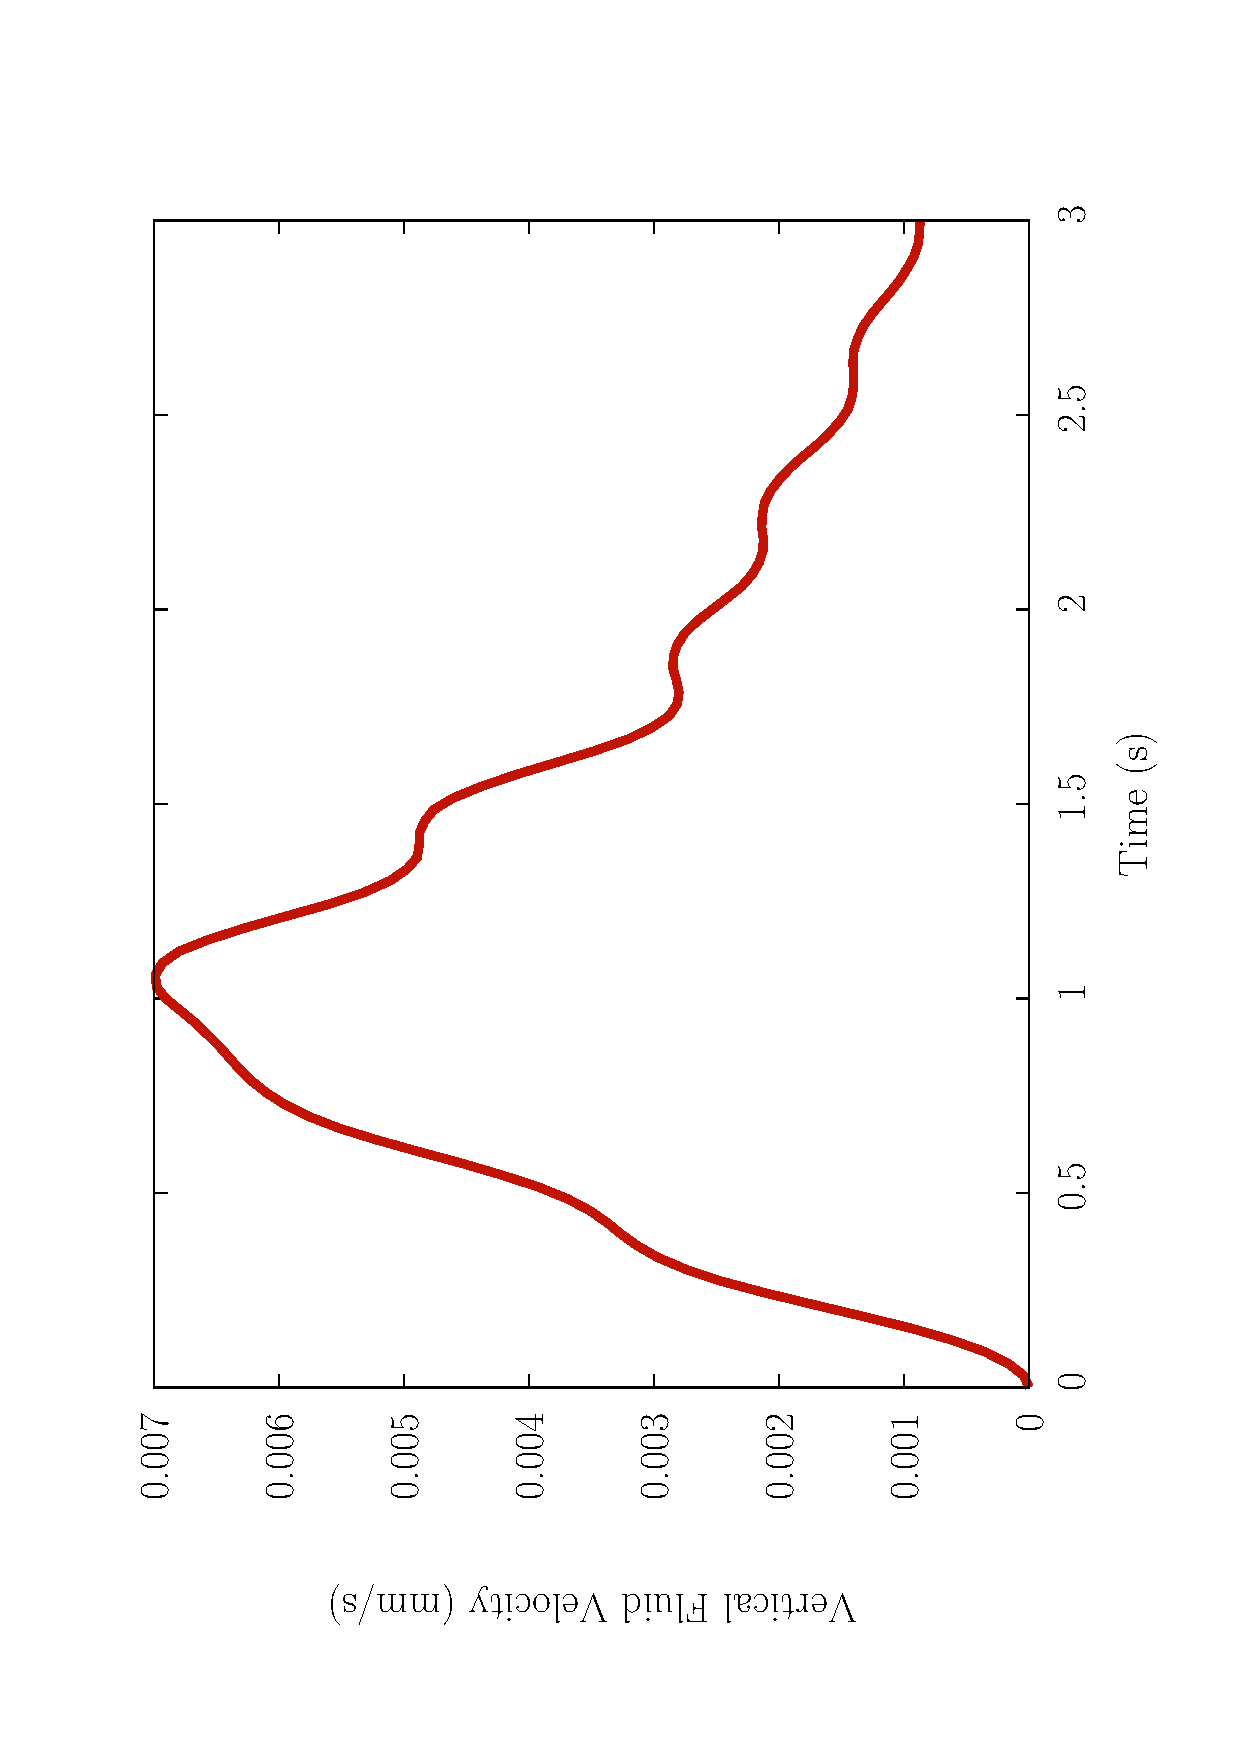
\includegraphics[width=0.6\textwidth,angle=270]{images/examples/%
eulerian/constriction/constrict-vel-drop-dynamic}
\caption{Vertical fluid velocity evolution with dynamics.} 
\label{velocity-evolution-dynamic}
\end{figure}

\begin{figure}[!hptb]
\centering
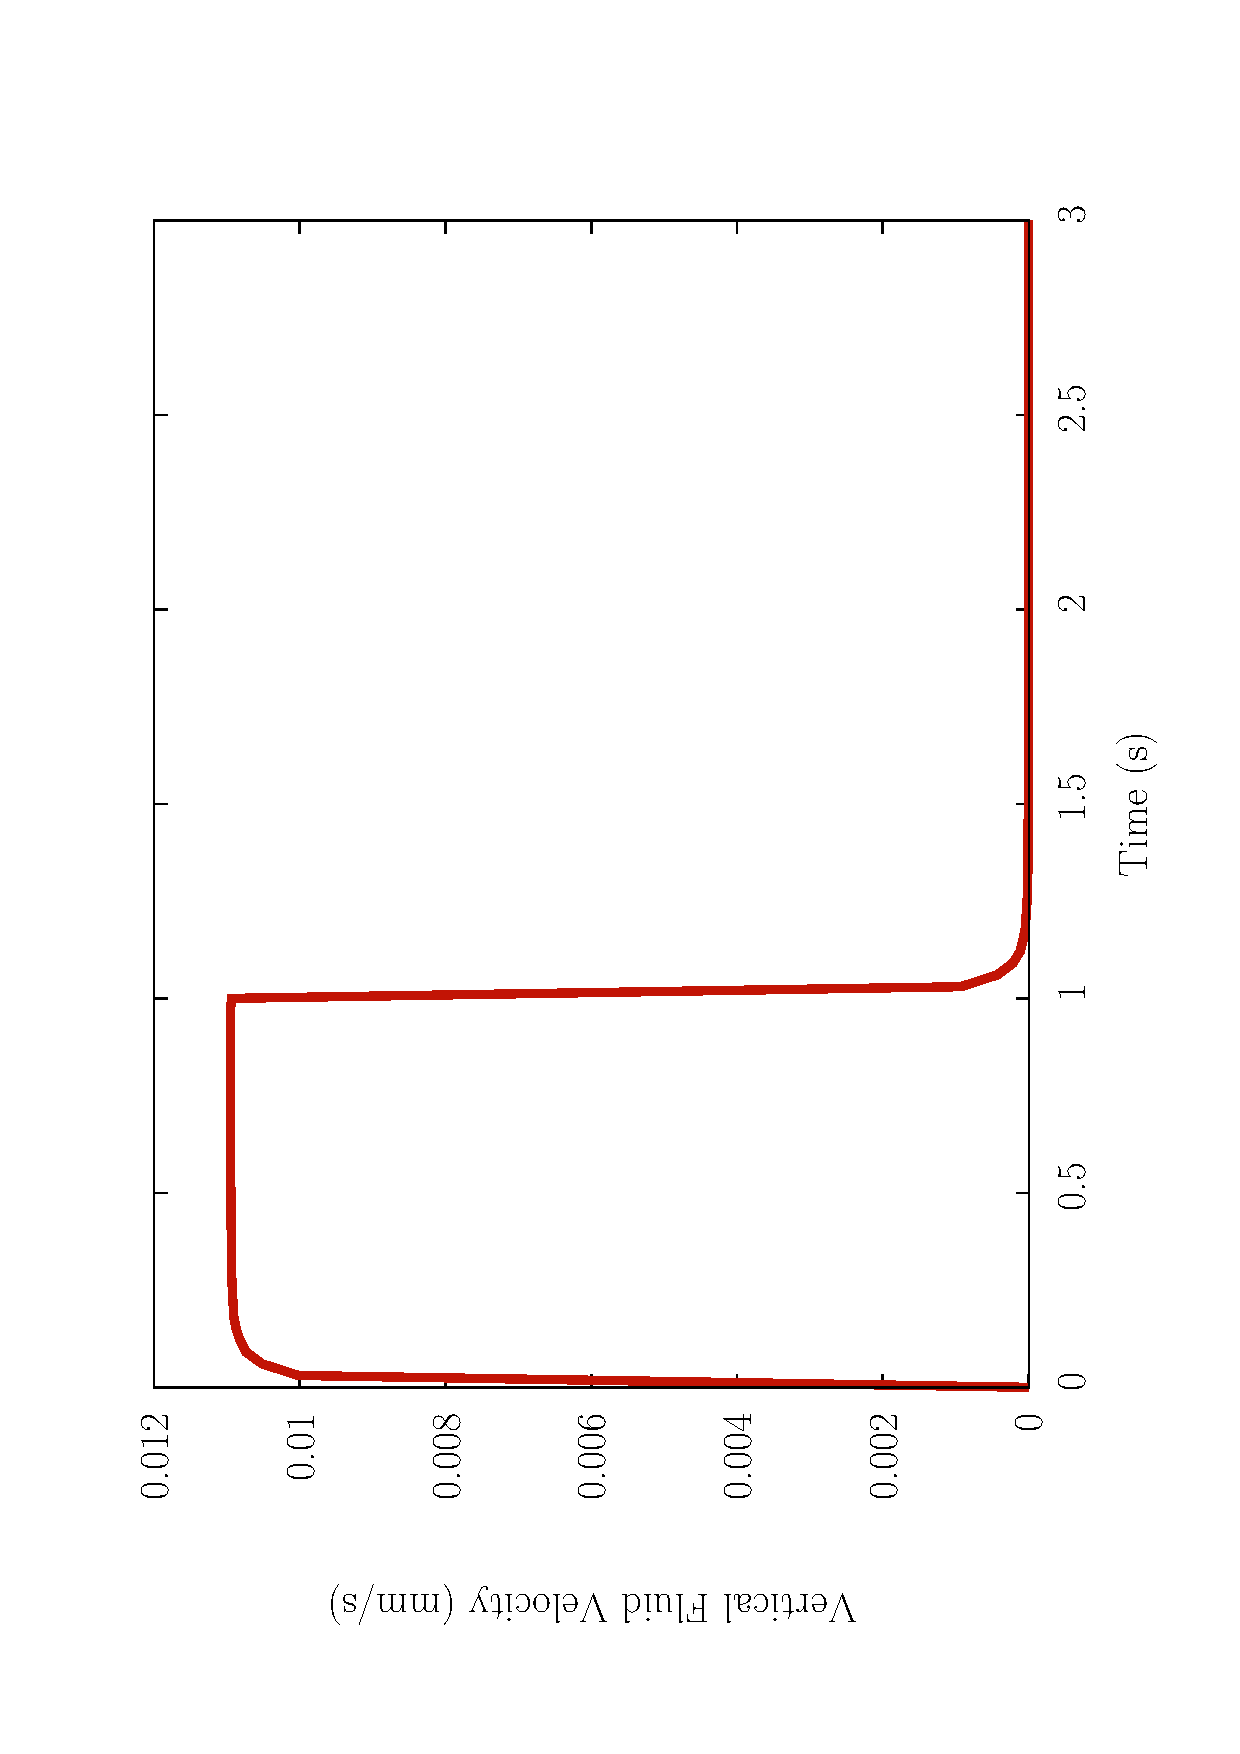
\includegraphics[width=0.6\textwidth,angle=270]{images/examples/%
eulerian/constriction/constrict-vel-drop-quasistatic}
\caption{Vertical fluid velocity evolution with quasistatics.} 
\label{velocity-evolution-quasistatic}
\end{figure}

\clearpage

\subsection{Flow fields under tension}
\label{tension-flow}

\textbullet\ Now that we're reasonably confident about the fluid flow
fields and have an idea of its effects on the mechanics, we proceed to
tailor the material model, geometry and constants to better represent
actual cases.

\section{Examples exploring the biphasic nature of porous soft tissue}
\label{biphasic-examples-2}

\subsection{Stress relaxation}
\label{stress-relaxation}

\textbullet\ Set up the boundary conditions relevant to the
case. Basically pull and hold, and no outflow at the top and
bottom.

\subsubsection{Under different rates of loading}
\label{modifying-load-rates}

\textbullet\ In order to differentiate the effect of load rate. The
results show, as expected, that the faster-pulled case is stiffer,
arising from the higher force from the frictional interaction term.

\begin{figure}[!hptb]
\centering
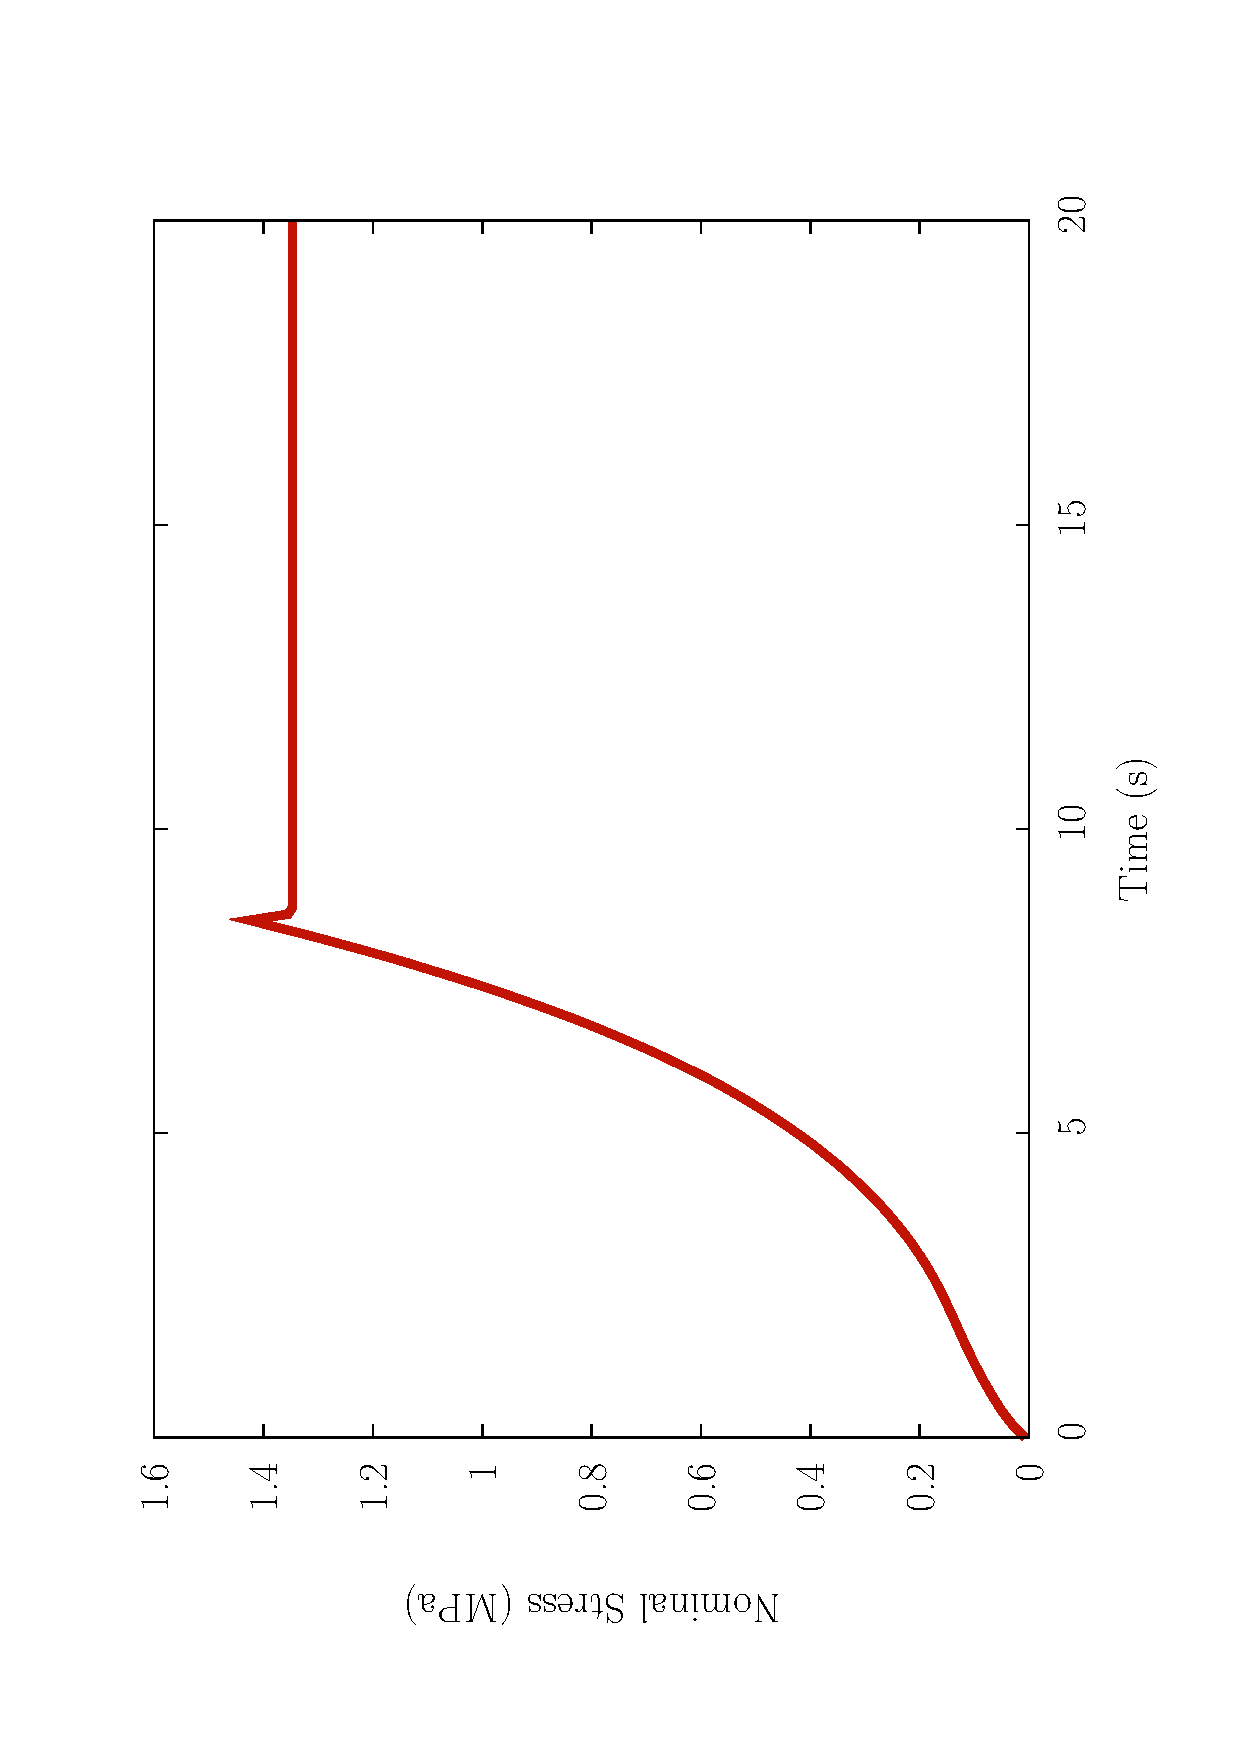
\includegraphics[width=0.6\textwidth,angle=270]{images/examples/%
eulerian/pulling/plots/poro-elastic/poro-stress-relax-0p01}
\caption{Dynamic poroelastic model, $\dot{\epsilon}=0.01$ Hz, $D=1.037$
  MPa.s.mm$^{-1}$.}
\label{poro-stress-relax-0p01}
\end{figure}

\begin{figure}[!hptb]
\centering
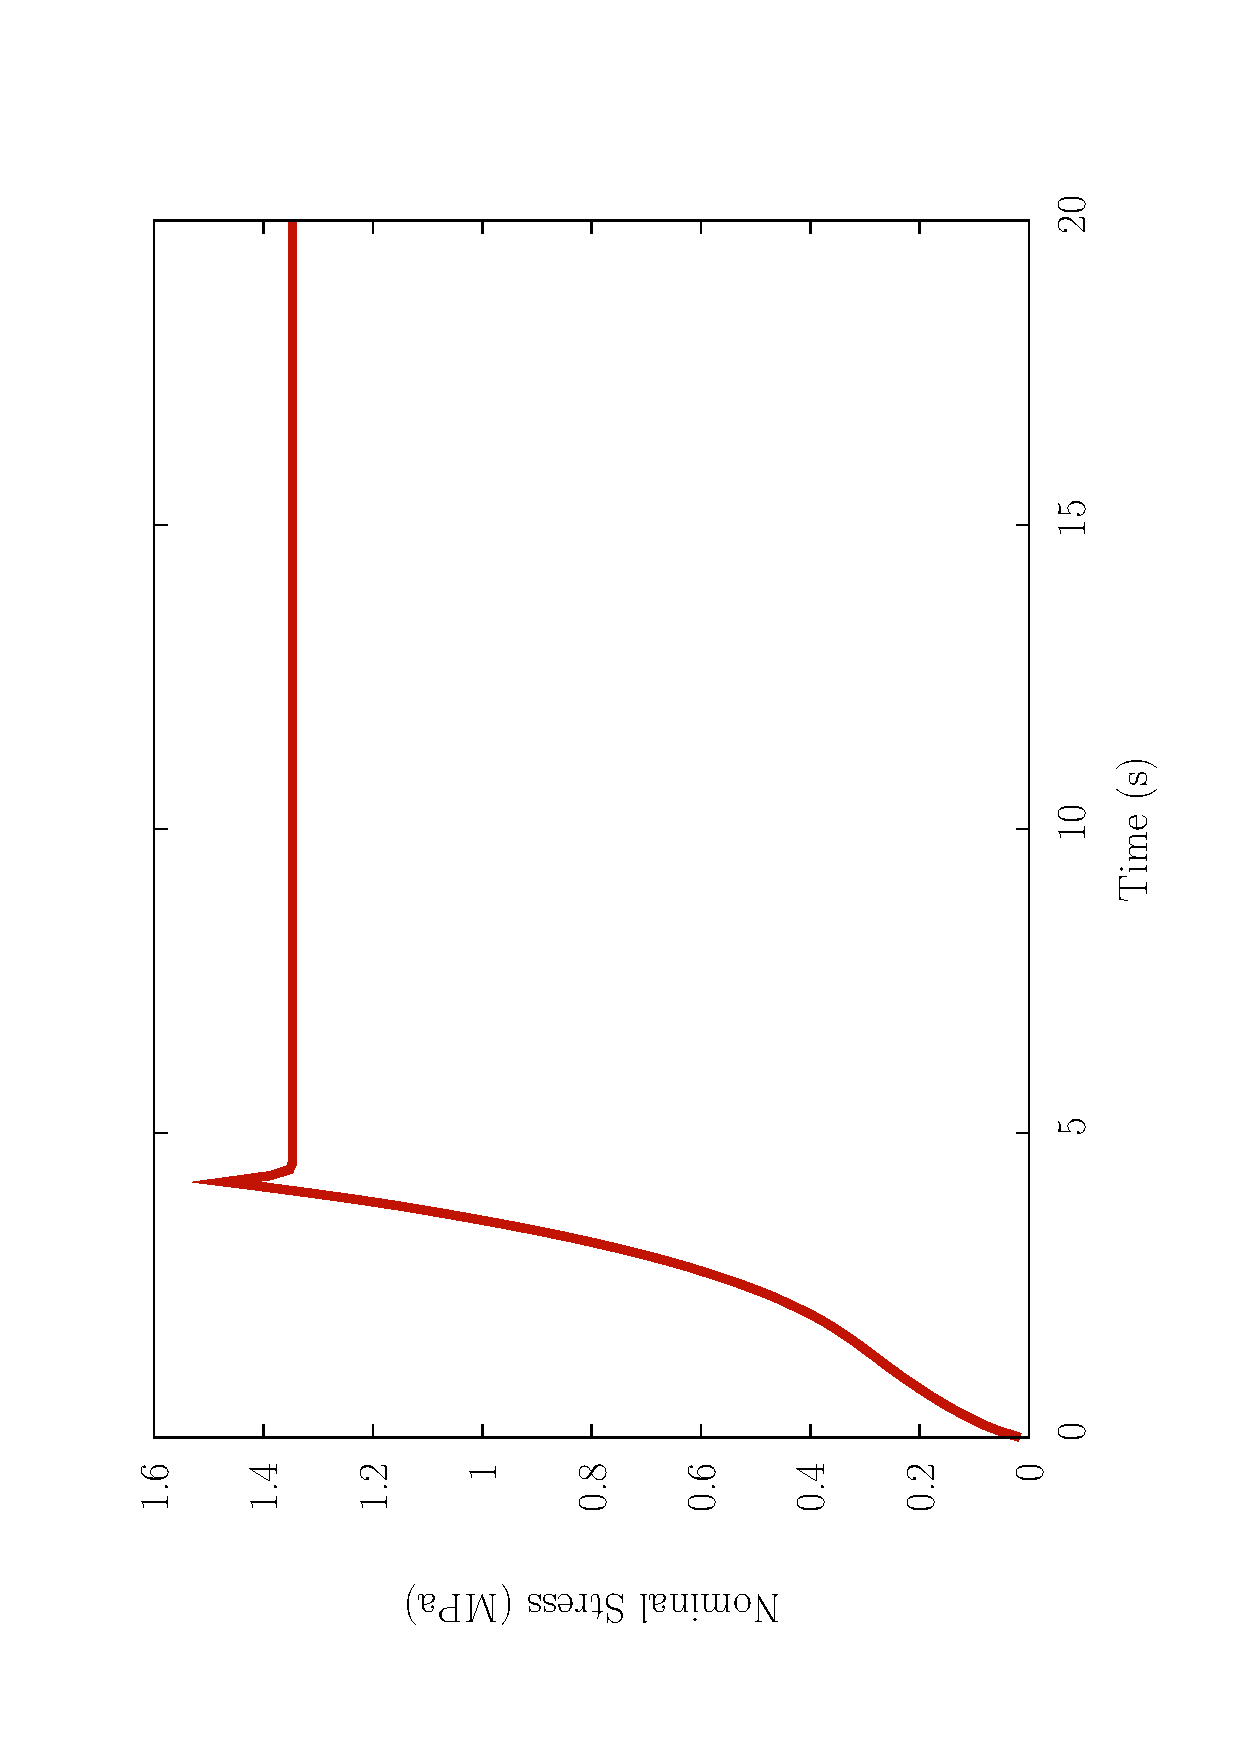
\includegraphics[width=0.6\textwidth,angle=270]{images/examples/%
eulerian/pulling/plots/poro-elastic/poro-stress-relax-0p02}
\caption{Dynamic poroelastic model, $\dot{\epsilon}=0.02$ Hz, $D=1.037$
  MPa.s.mm$^{-1}$.}
\label{poro-stress-relax-0p02}
\end{figure}

\subsubsection{Comparison with representative viscoelastic curves}
\label{viscoelastic-stress-relaxation}

\textbullet\ This calculation uses a linear-viscoelastic model and is
presented for qualitative comparison. We're interested, as mentioned
in a Section before, in the inelastic behaviour of tissues. The goal
of these examples are not to solve the final problem, but to show that
different cases can be solved reasonably within the framework and show
different results qualitatively and quantitatively. Notice that the
viscoelastic curve does the same general thing.

\begin{figure}[!hptb]
\centering
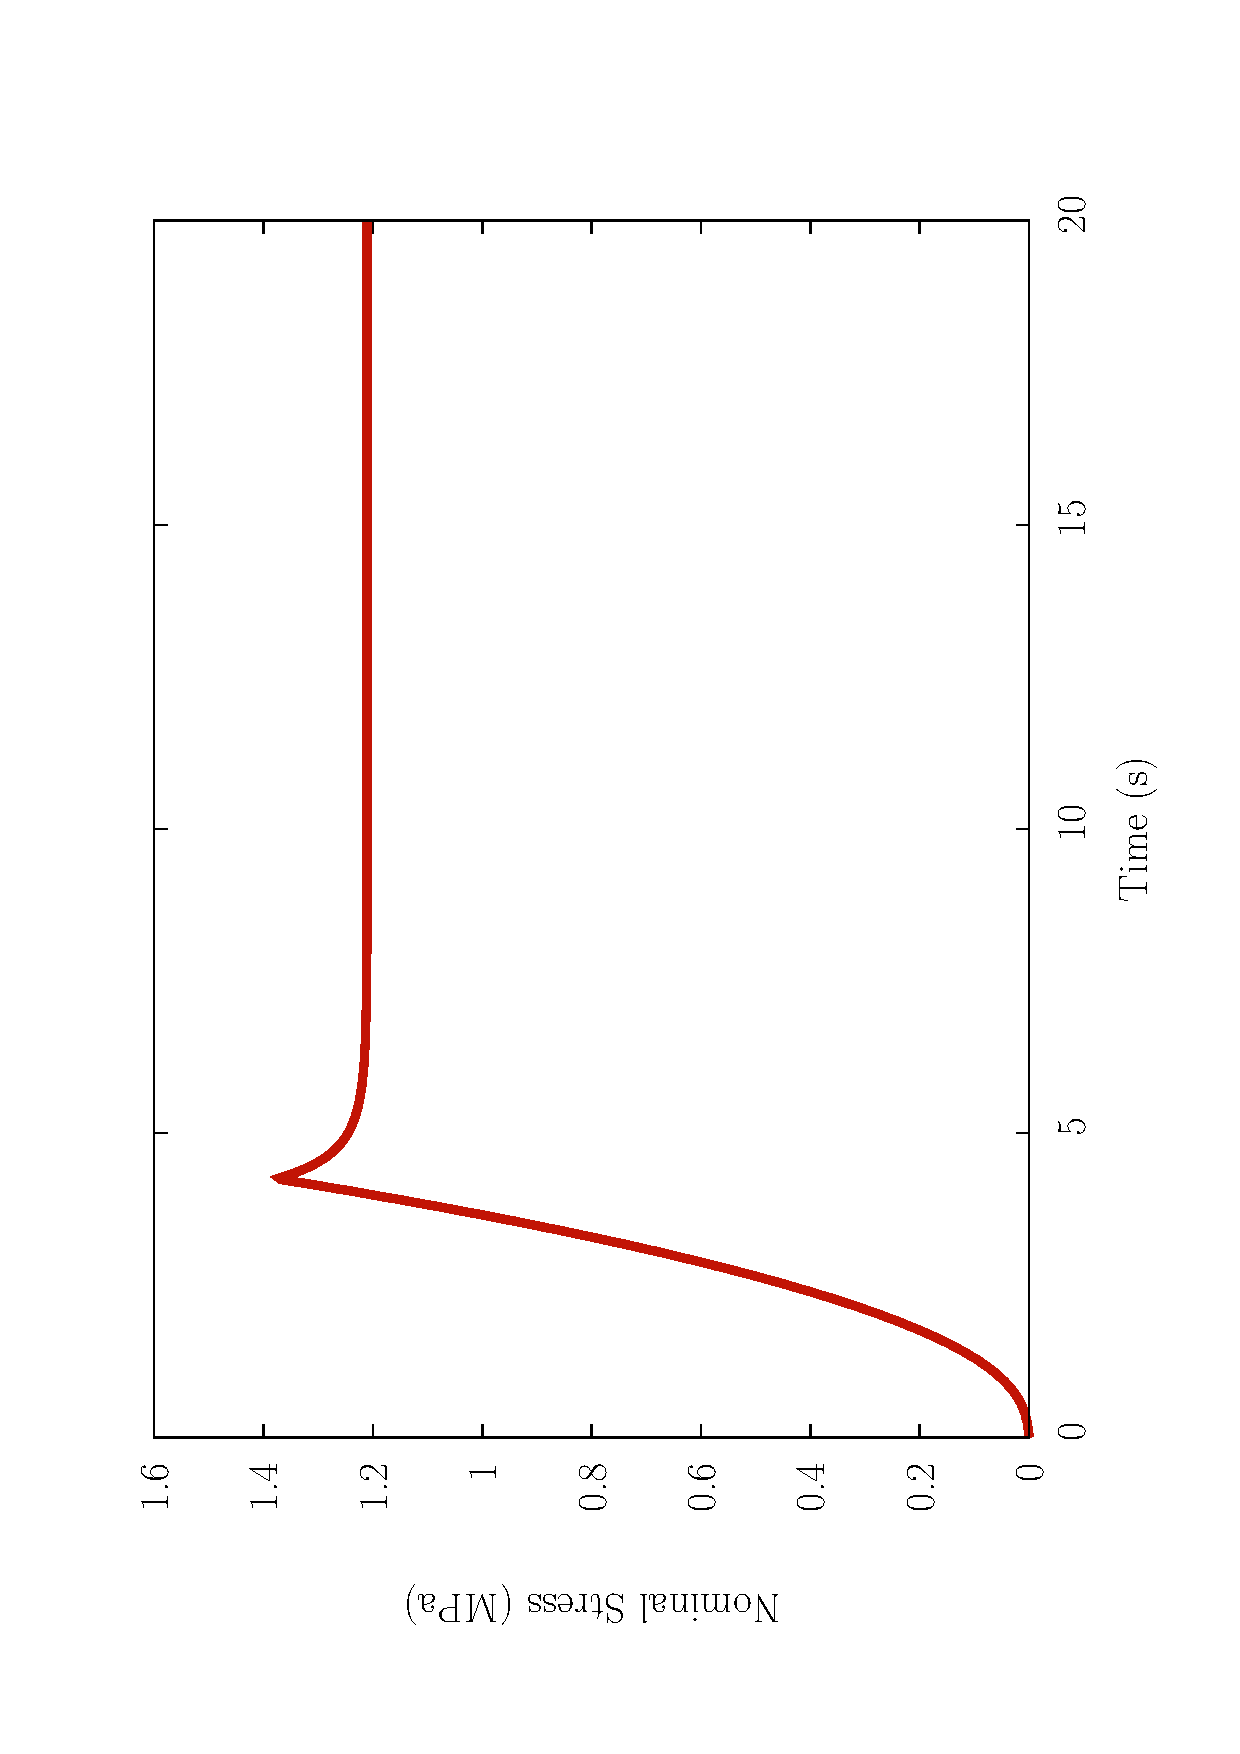
\includegraphics[width=0.6\textwidth,angle=270]{images/examples/%
eulerian/pulling/plots/visco-elastic/visco-stress-relax-0p02-t0p3}
\caption{Dynamic viscoelastic model, $\dot{\epsilon}=0.02$ Hz,
  $\tau=0.3$ s.}
\label{visco-stress-relax-0p02-t0p3}
\end{figure}

\textbullet\ Also, the nonlinear case can also be trivially handled,
and it's comparison with experiment is shown below.

\subsubsection{Non-linear viscoelasticity}
\label{non-linear-viscoelasticity}

\begin{figure}[!hptb]
\centering
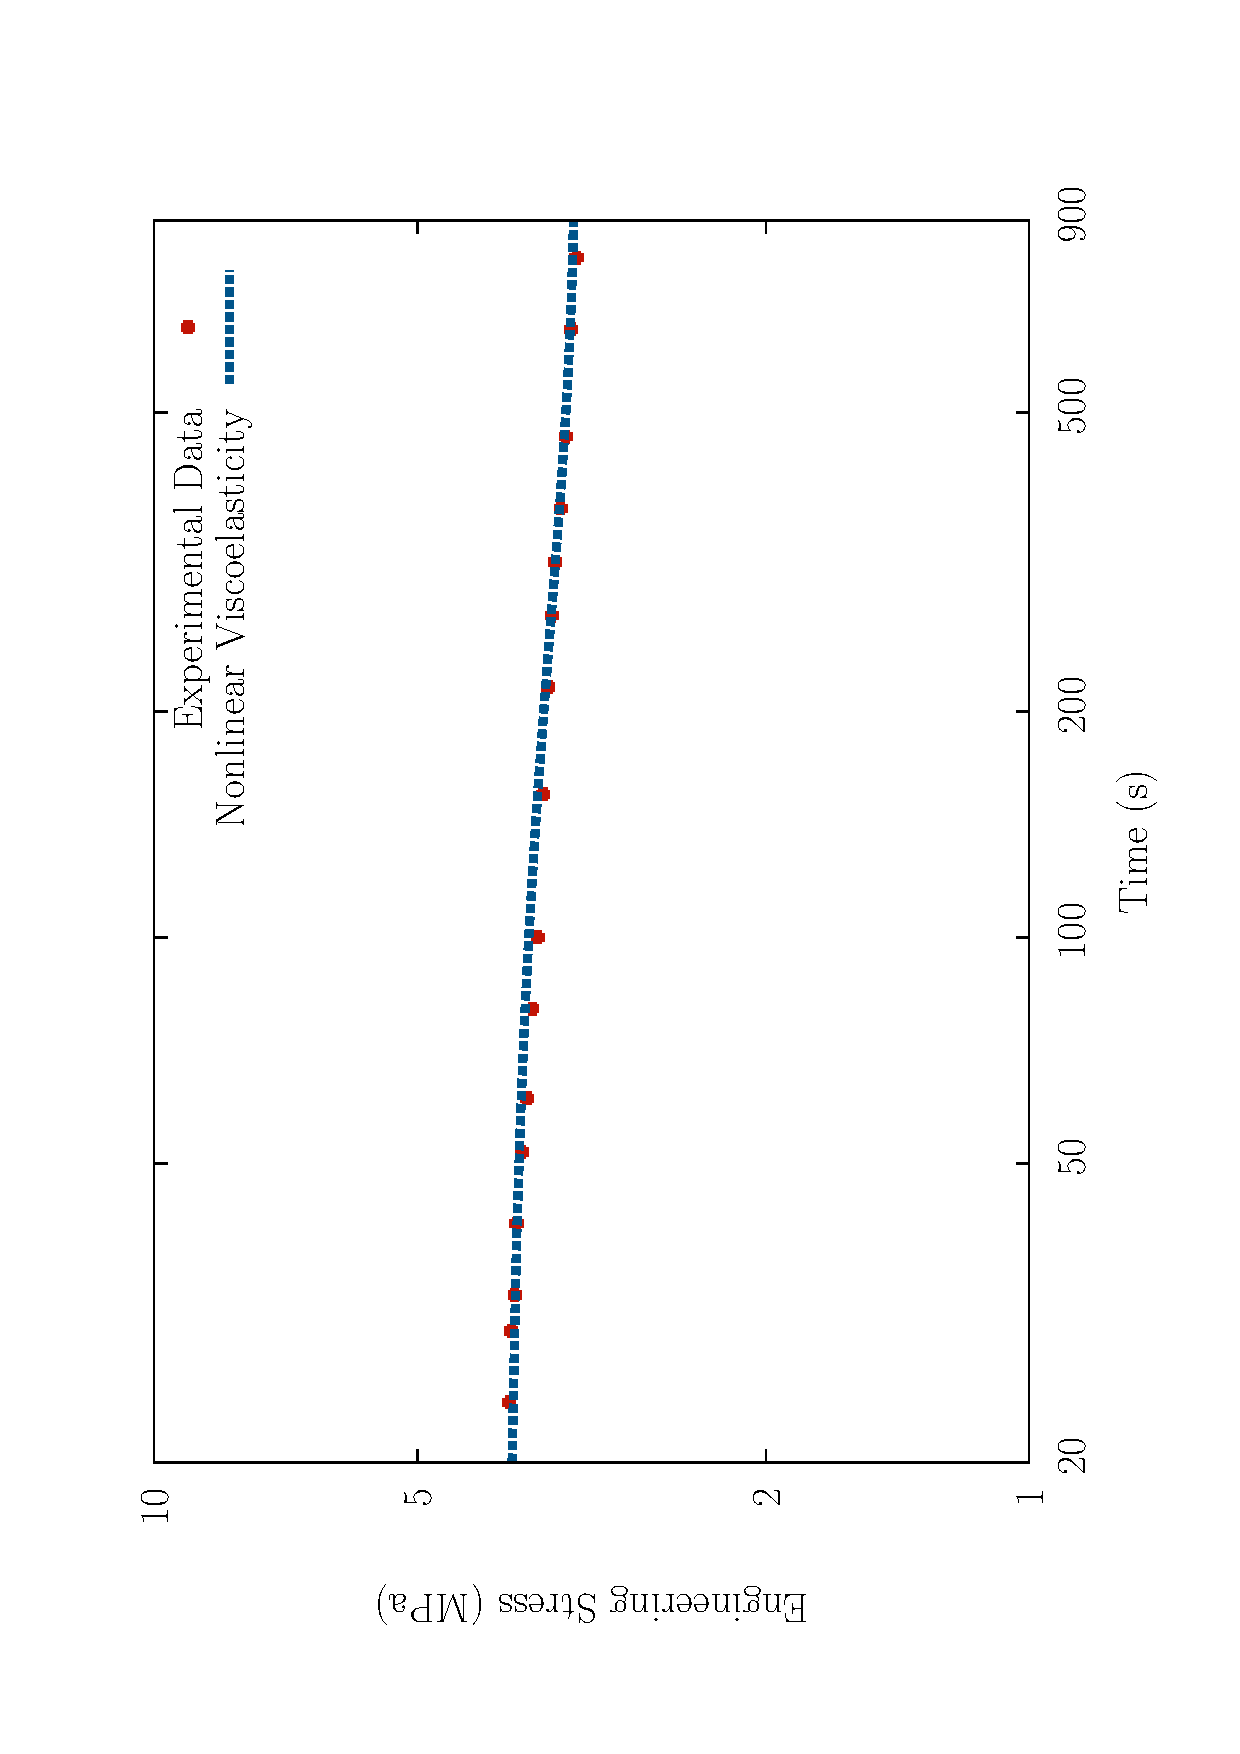
\includegraphics[width=0.6\textwidth,angle=270]{images/examples/%
eulerian/nonlinear-viscoelasticity/provenzano-data-comparison}
\caption{The non-linear time constants fit to experiment.} 
\label{provenzano-data-fit}
\end{figure}

\begin{figure}[!hptb]
\centering
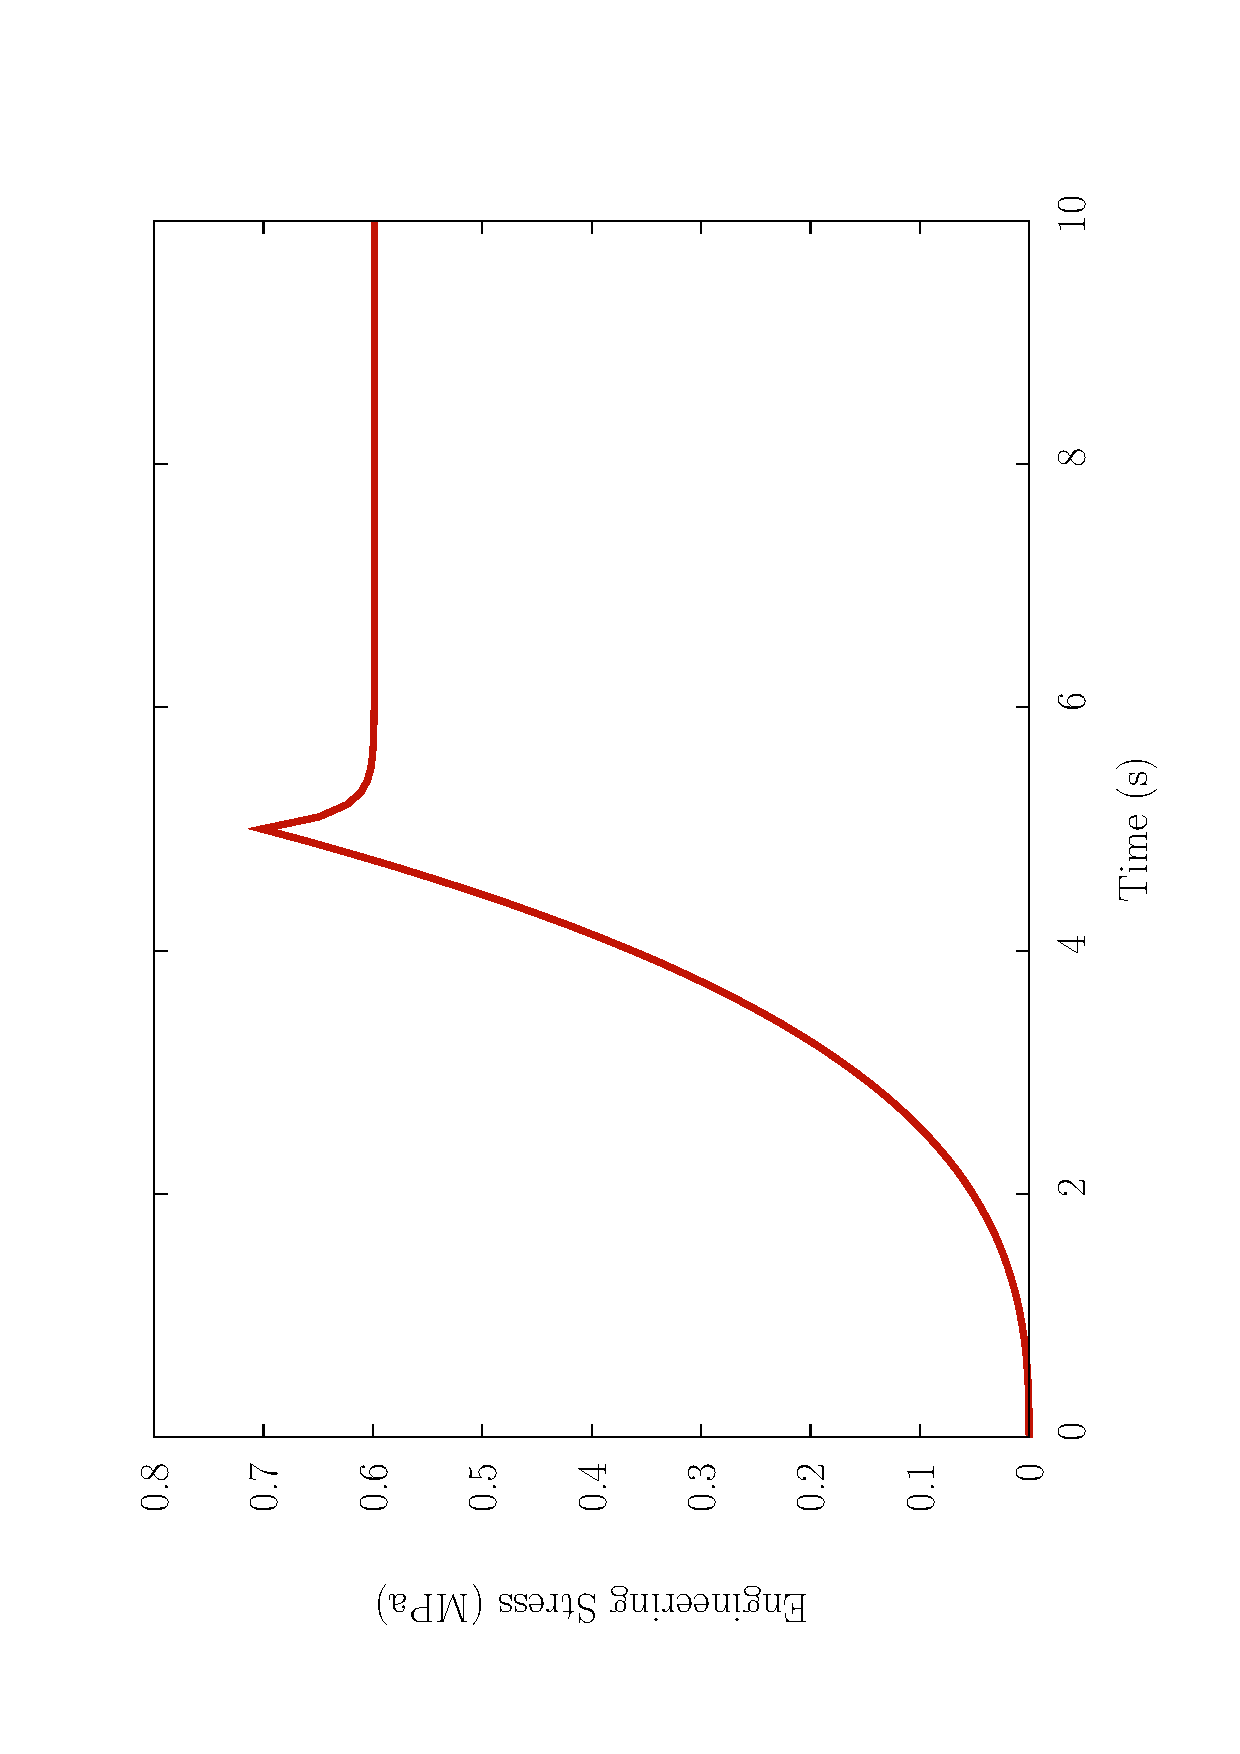
\includegraphics[width=0.6\textwidth,angle=270]{images/examples/%
eulerian/nonlinear-viscoelasticity/nonlinear-viscoelasticity-stress-relaxation}
\caption{Stress relaxation under nonlinear viscoelasticity.}
\label{nonlinear-viscoelasticity-stress-relaxation}
\end{figure}

\clearpage

\subsection{Hysteresis in the cyclic stress-strain response}
\label{hysteresis}

\textbullet\ Now that we've established a simple pull and hold, we
move onto a more complicated pull and unload. Talk about the boundary
conditions and perhaps provide the 2 experimental results first?

\textbullet\ Since quasistatic and dynamic were found important, we
look at those two cases for a certain ratio of fluid to
solid. Clearly, there is a difference.

\subsubsection{Quasistatic vs. dynamic}
\label{quasistatic-vs-dynamic}

\begin{figure}[!hptb]
\centering
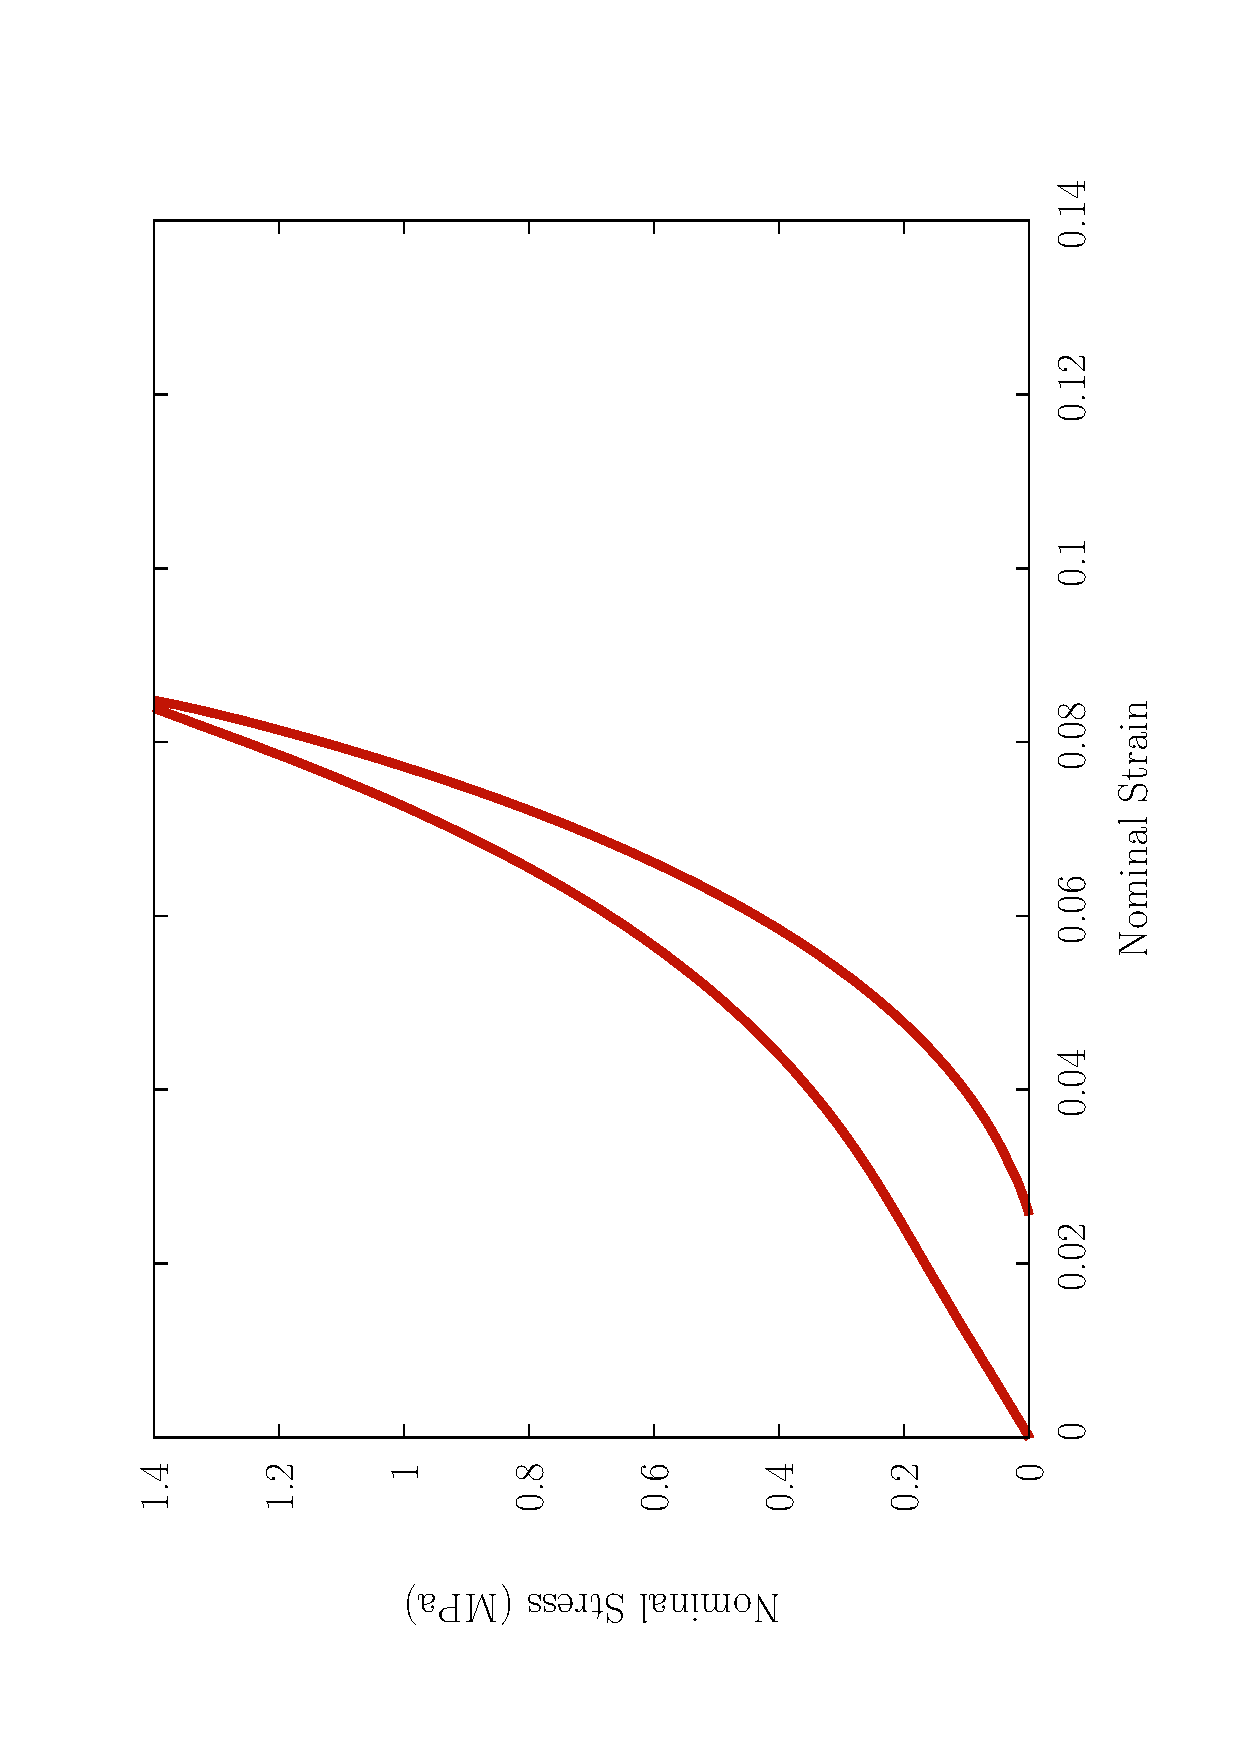
\includegraphics[width=0.6\textwidth,angle=270]{images/examples/%
eulerian/pulling/plots/poro-elastic/medium-hysteresis-static-0p01-d1p037}
\caption{Quasistatic poroelastic model, $\dot{\epsilon}=0.01$ Hz, $D=1.037$
  MPa.s.mm$^{-1}$.}
\label{medium-hysteresis-static-0p01-d1p037}
\end{figure}

\begin{figure}[!hptb]
\centering
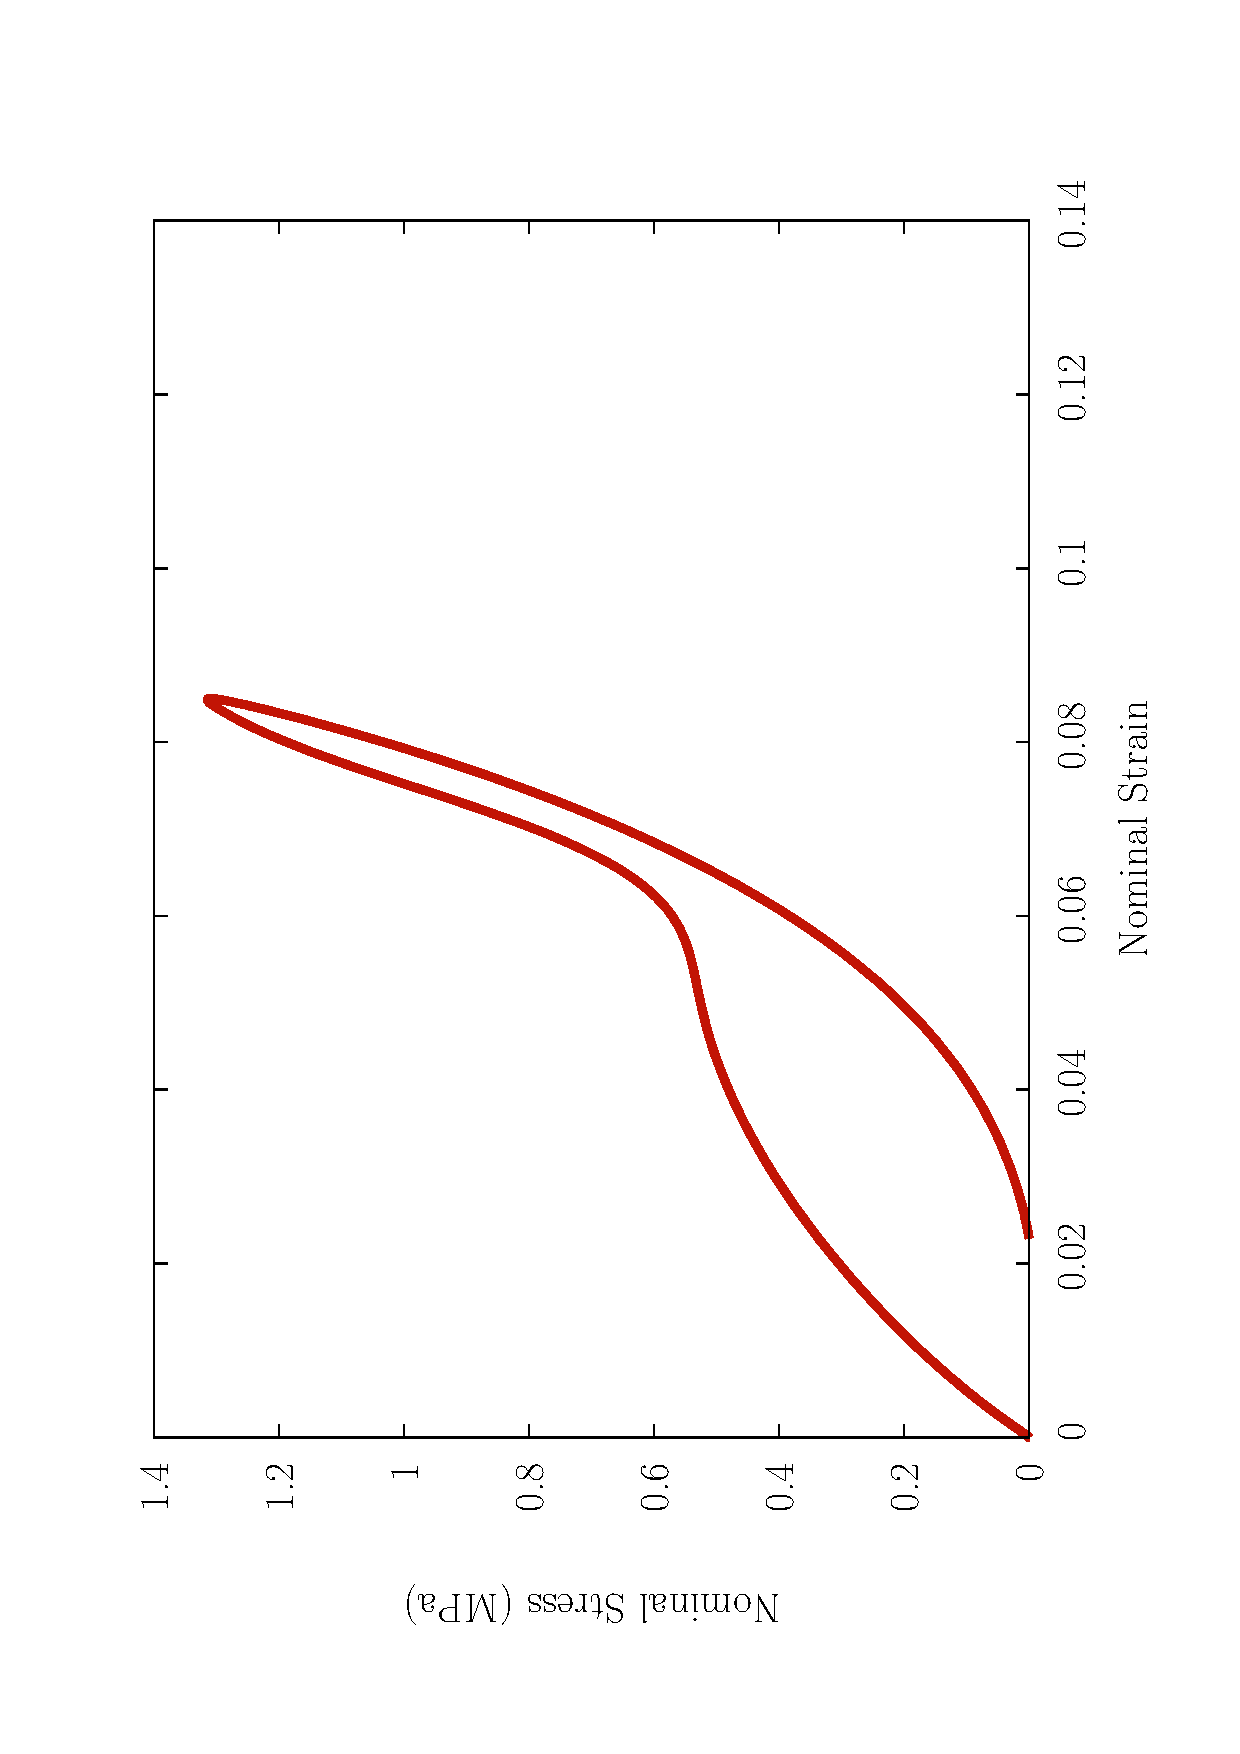
\includegraphics[width=0.6\textwidth,angle=270]{images/examples/%
eulerian/pulling/plots/poro-elastic/medium-hysteresis-dynamic-0p01-d1p037}
\caption{Dynamic poroelastic model, $\dot{\epsilon}=0.01$ Hz, $D=1.037$
  MPa.s.mm$^{-1}$.}
\label{medium-hysteresis-dynamic-0p01-d1p037}
\end{figure}

\textbullet\ Note that the fluid-sloshy-effects go away during the
higher strain ranges where the solid is substantially stiffer.

\subsubsection{Changing load-rates and friction coefficients}
\label{load-rates-and-friction-coefficients}

\textbullet\ We now proceed to change the load rates/friction
coefficients in order to observe effects. Clearly, slower tests tend
the process toward equilibrium and it tends to become elastic,
reducing the dissipation and area under the curve.

\textbullet\ With the fluid (relative) velocities fixed (by the
boundary conditions), increasing
the frictional coefficient 10-fold increases the effects of the
fluid-sloshing dynamics substantially.

\begin{figure}[!hptb]
\centering
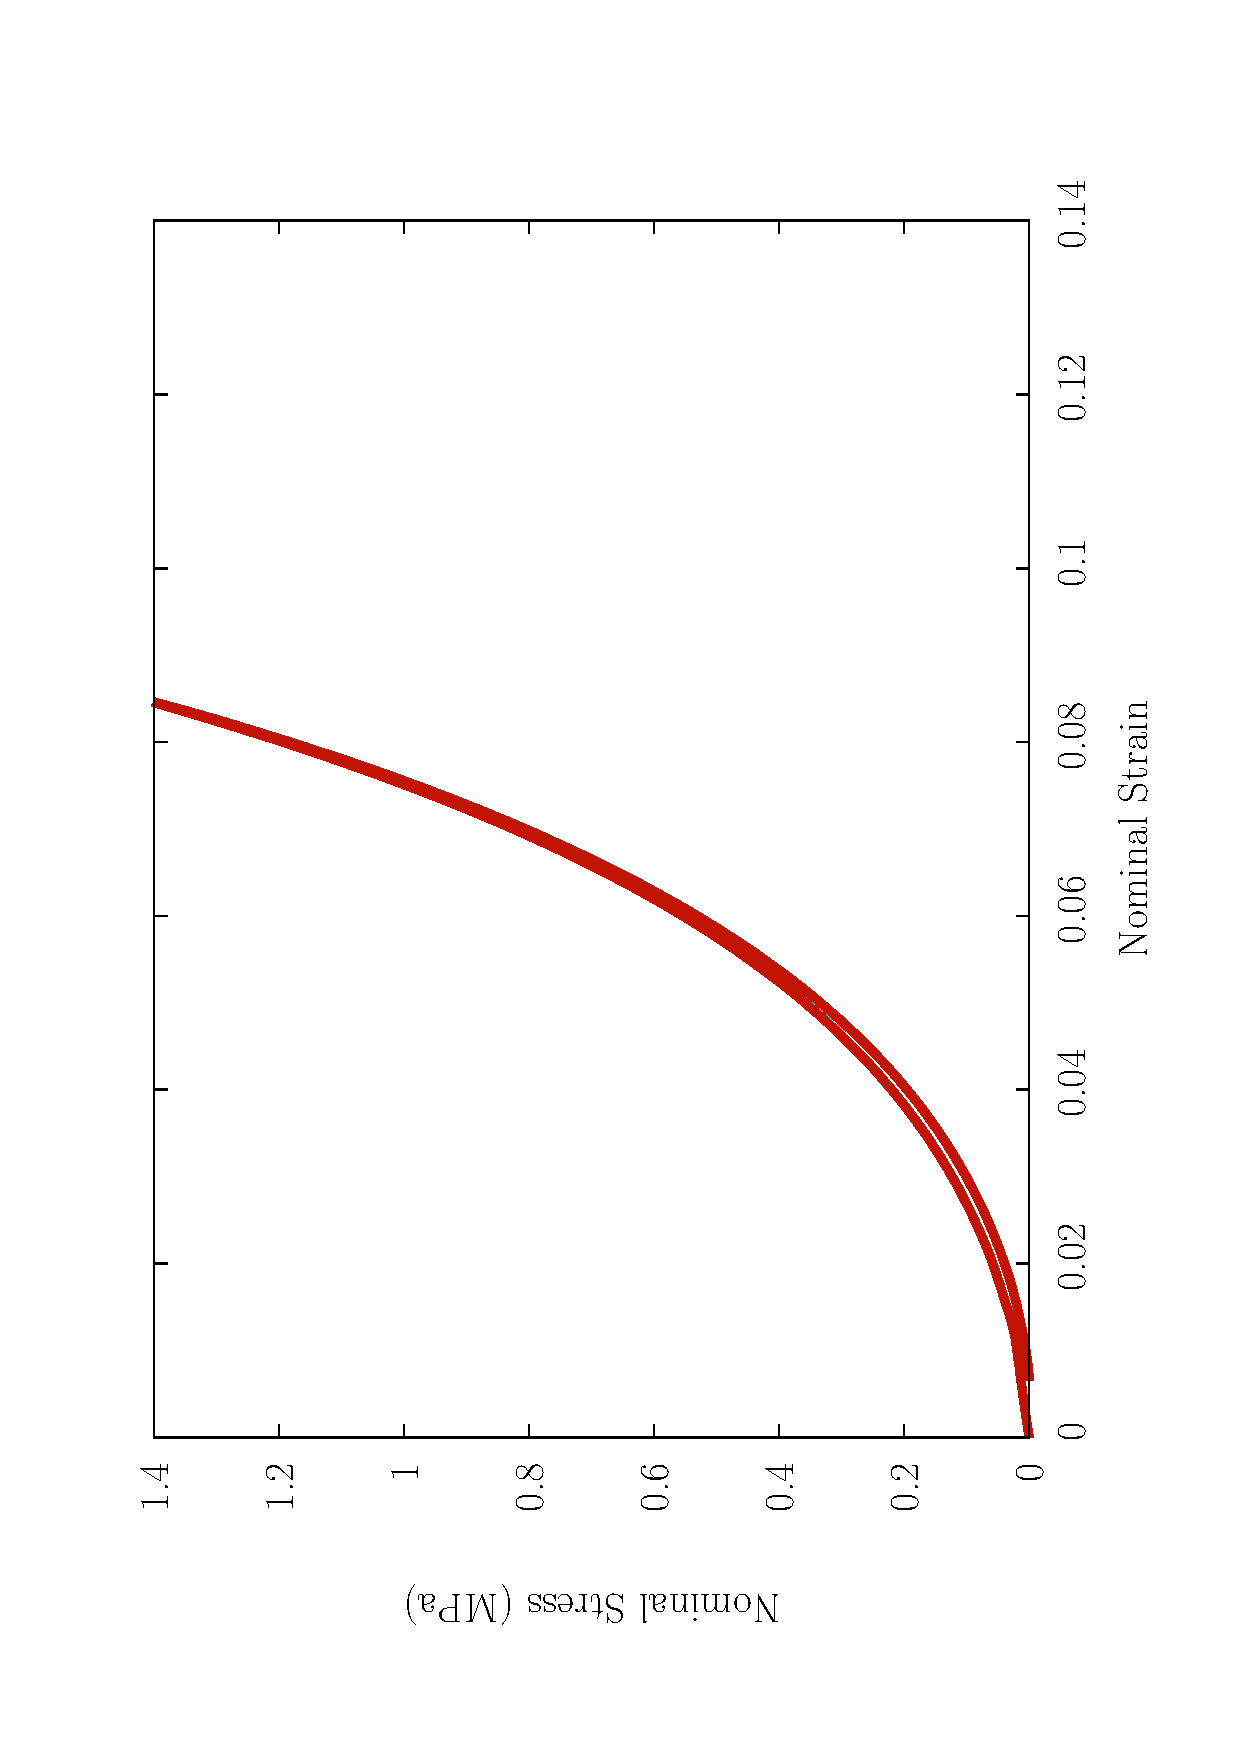
\includegraphics[width=0.6\textwidth,angle=270]{images/examples/%
eulerian/pulling/plots/poro-elastic/medium-hysteresis-dynamic-0p001-d1p037}
\caption{Dynamic poroelastic model, $\dot{\epsilon}=0.001$ Hz, $D=1.037$
  MPa.s.mm$^{-1}$.}
\label{medium-hysteresis-dynamic-0p001-d1p037}
\end{figure}

\begin{figure}[!hptb]
\centering
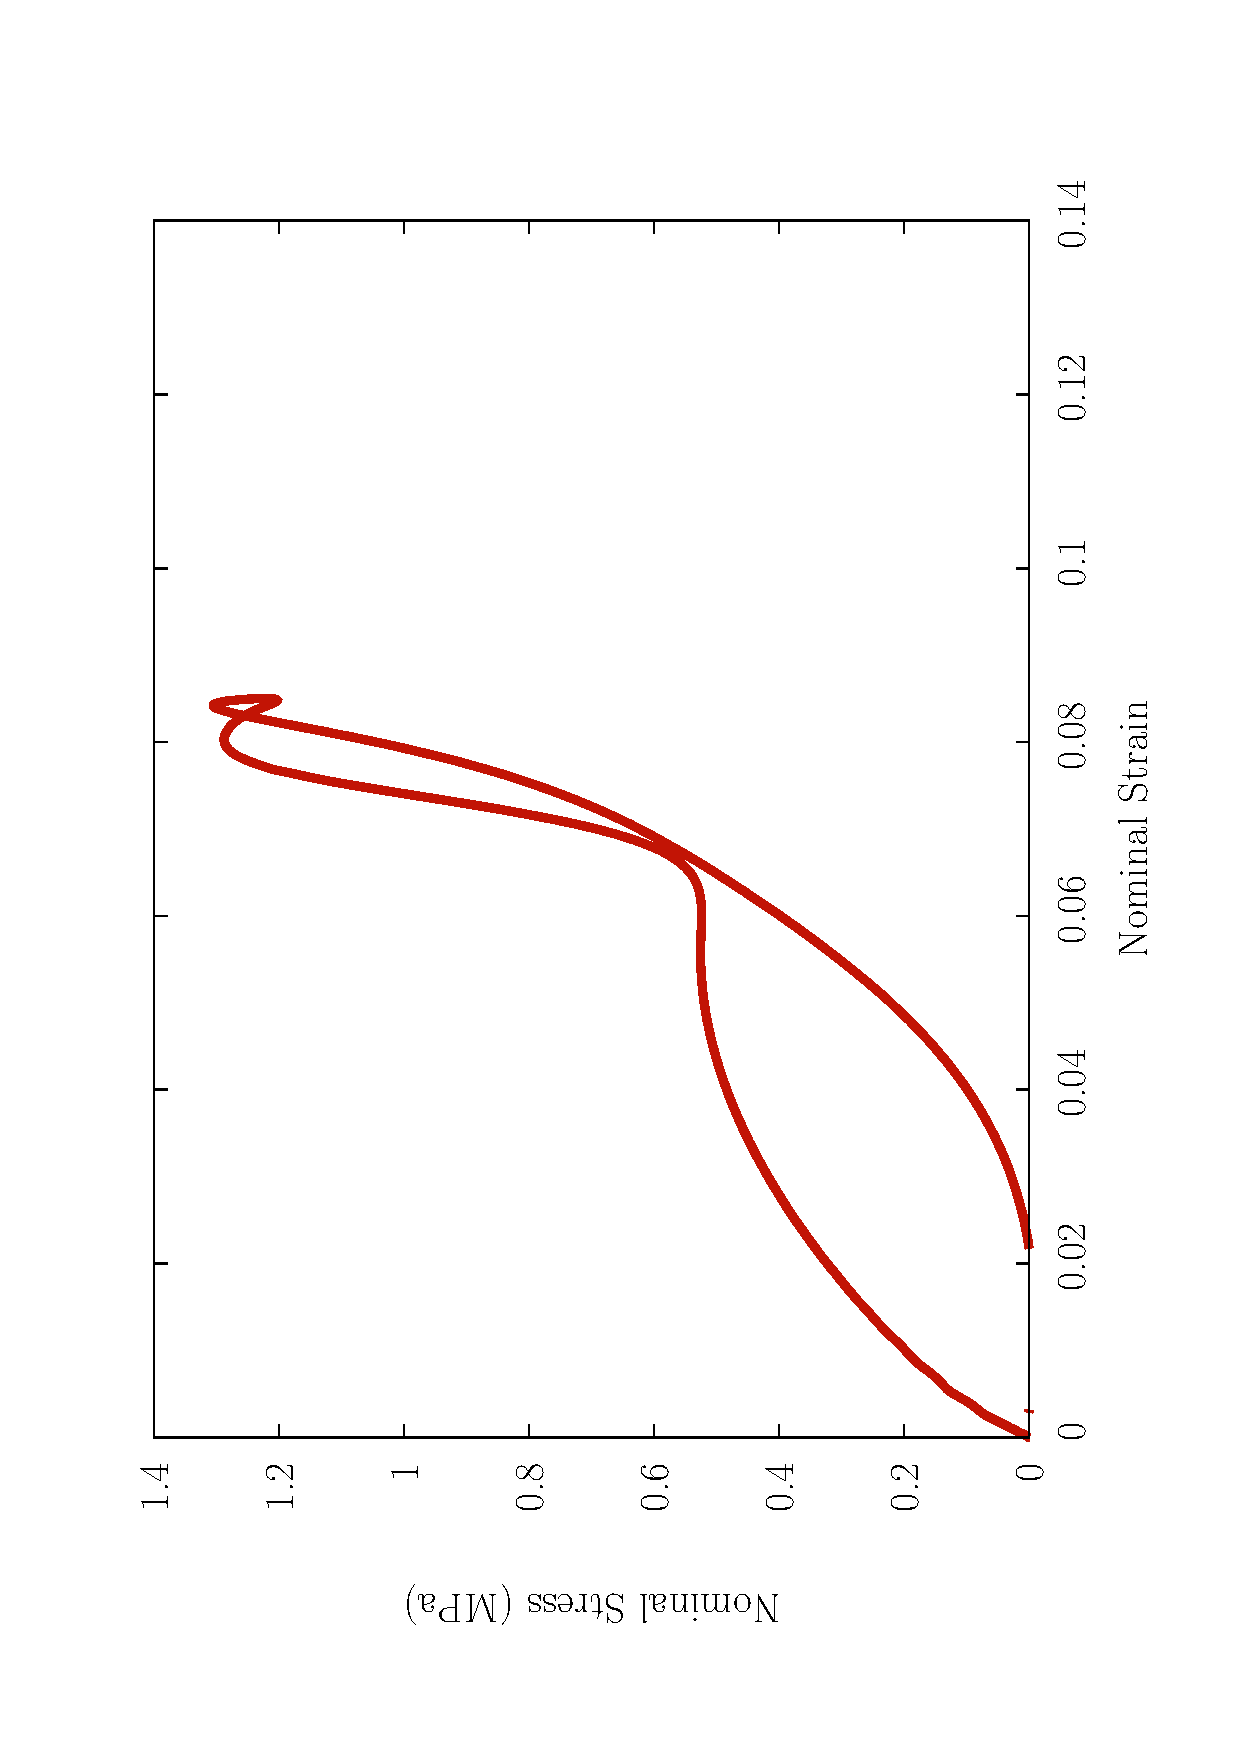
\includegraphics[width=0.6\textwidth,angle=270]{images/examples/%
eulerian/pulling/plots/poro-elastic/medium-hysteresis-dynamic-0p01-d10p37}
\caption{Dynamic poroelastic model, $\dot{\epsilon}=0.01$ Hz, $D=10.37$
  MPa.s.mm$^{-1}$.}
\label{medium-hysteresis-dynamic-0p01-d10p37}
\end{figure}

\subsubsection{Changing the overall shape and stress range}
\label{changing-shape}

\textbullet\ All the plots shown thus far have had the same general
shape, but experiments show different things for different tissues at
different ages. We can easily model this by changing the material
parameters to change the stress-ranges and shapes.

\begin{figure}[!hptb]
\centering
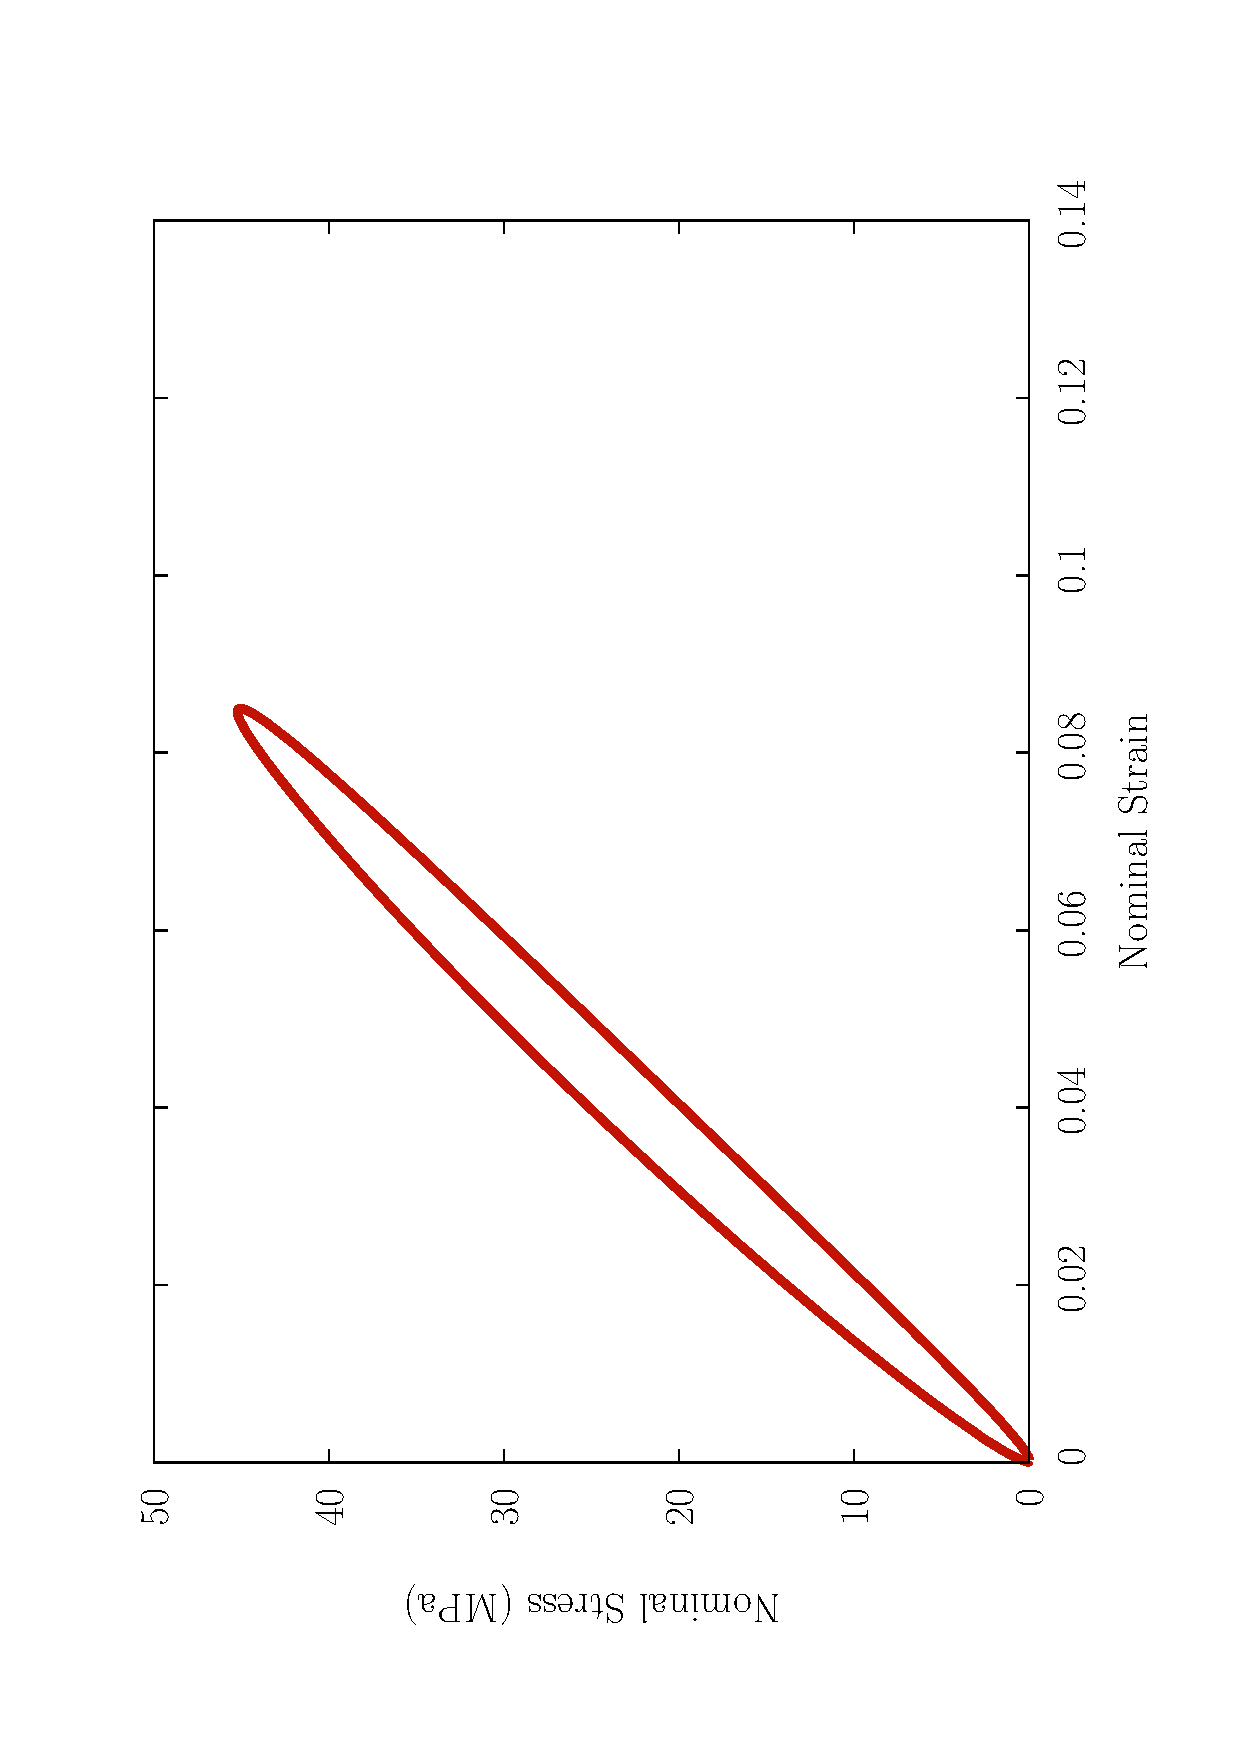
\includegraphics[width=0.6\textwidth,angle=270]{images/examples/%
eulerian/pulling/plots/poro-elastic/low-hysteresis-dynamic-0p01-d1p037}
\caption{Dynamic poroelastic model, $\dot{\epsilon}=0.01$ Hz, $D=1.037$
  MPa.s.mm$^{-1}$.}
\label{low-hysteresis-dynamic-0p01-d1p037}
\end{figure}

\subsubsection{Comparison with representative linear viscoelastic
  curves}
\label{viscoelastic-hysteresis}

And, to compare, here are two plots (one for each set of material
properties) using a linear viscoelastic model. Clearly, the visco case
misses the noisyness arising from fluid-sloshing which the poro case
captures. Therefore, combinations must be explored.

\begin{figure}[!hptb]
\centering
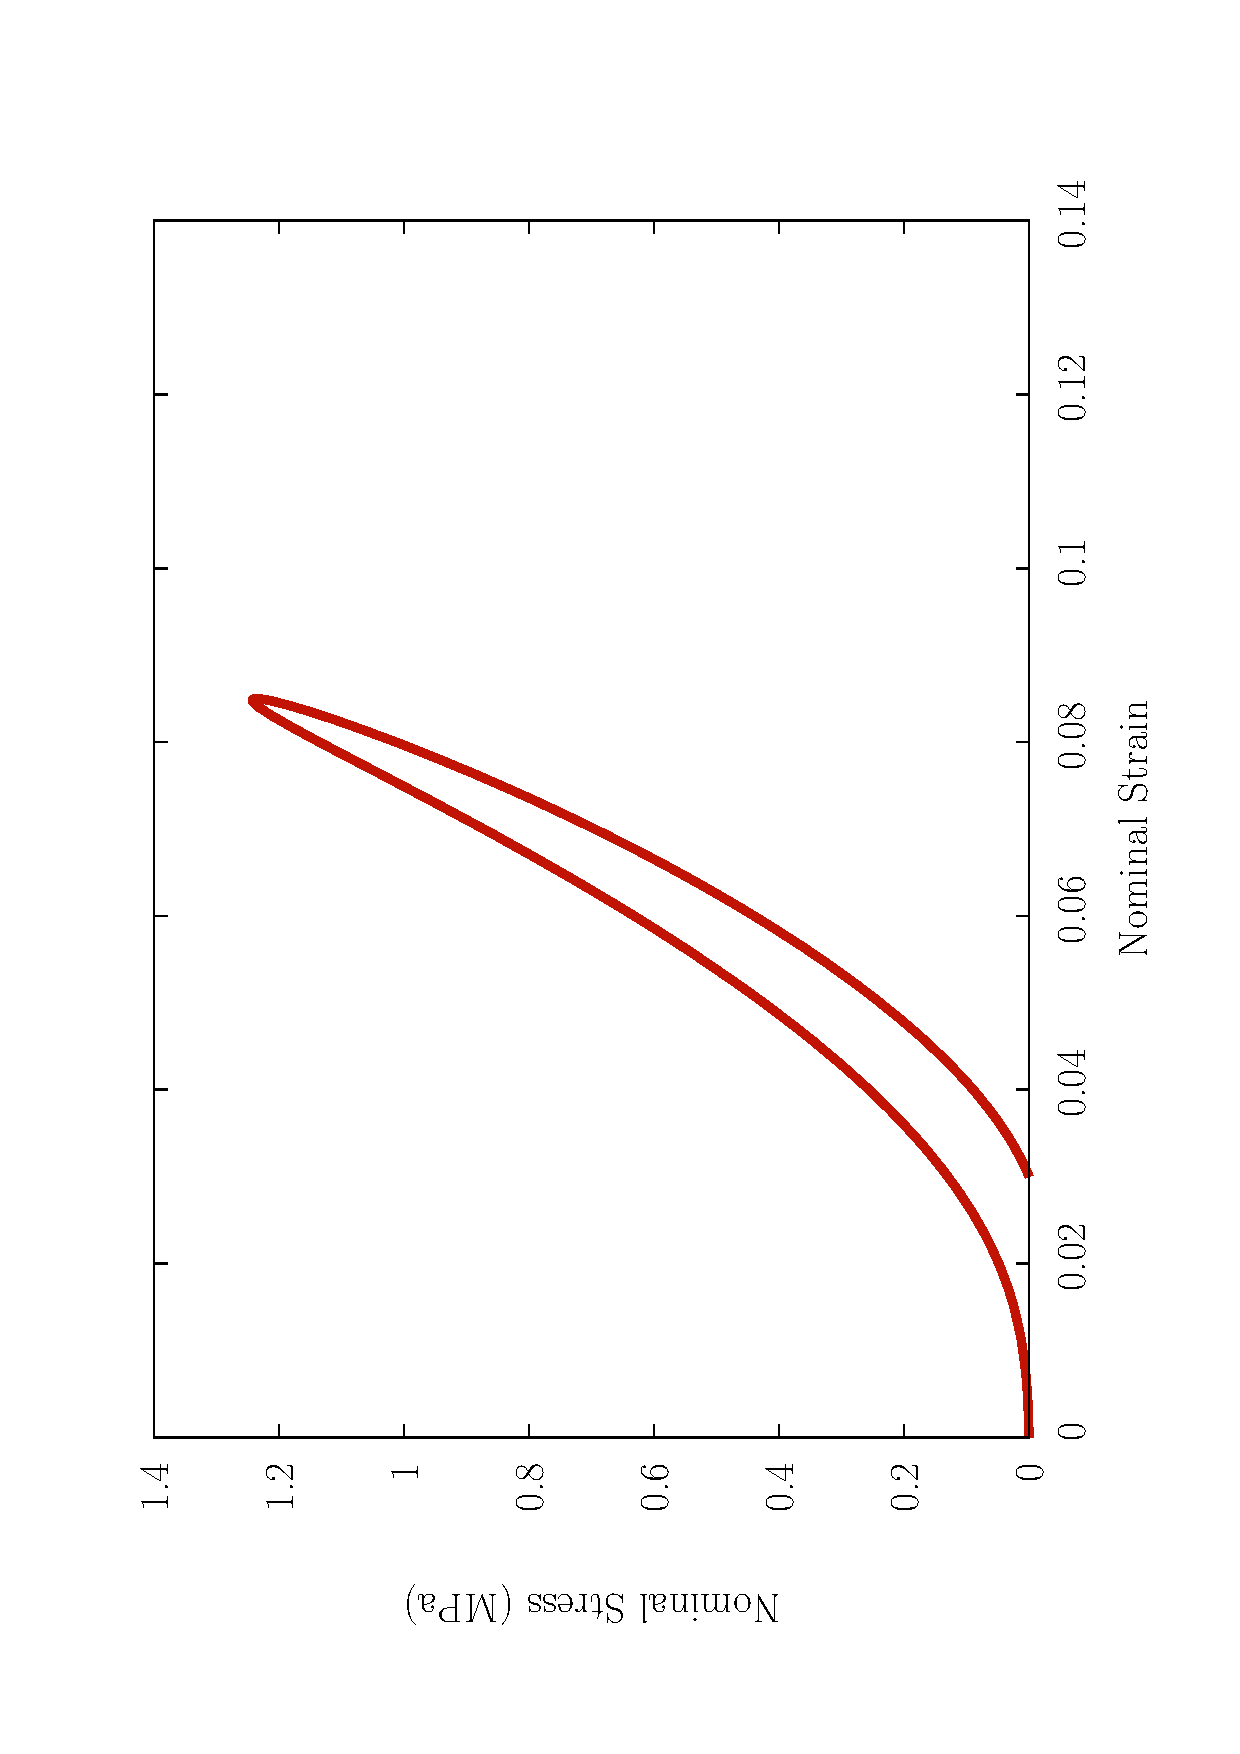
\includegraphics[width=0.6\textwidth,angle=270]{images/examples/%
eulerian/pulling/plots/visco-elastic/medium-hysteresis-visco-0p01-t0p3}
\caption{Dynamic viscoelastic model, $\dot{\epsilon}=0.01$ Hz,
  $\tau=0.3$ s.}
\label{medium-hysteresis-visco-0p01-t0p3}
\end{figure}

\begin{figure}[!hptb]
\centering
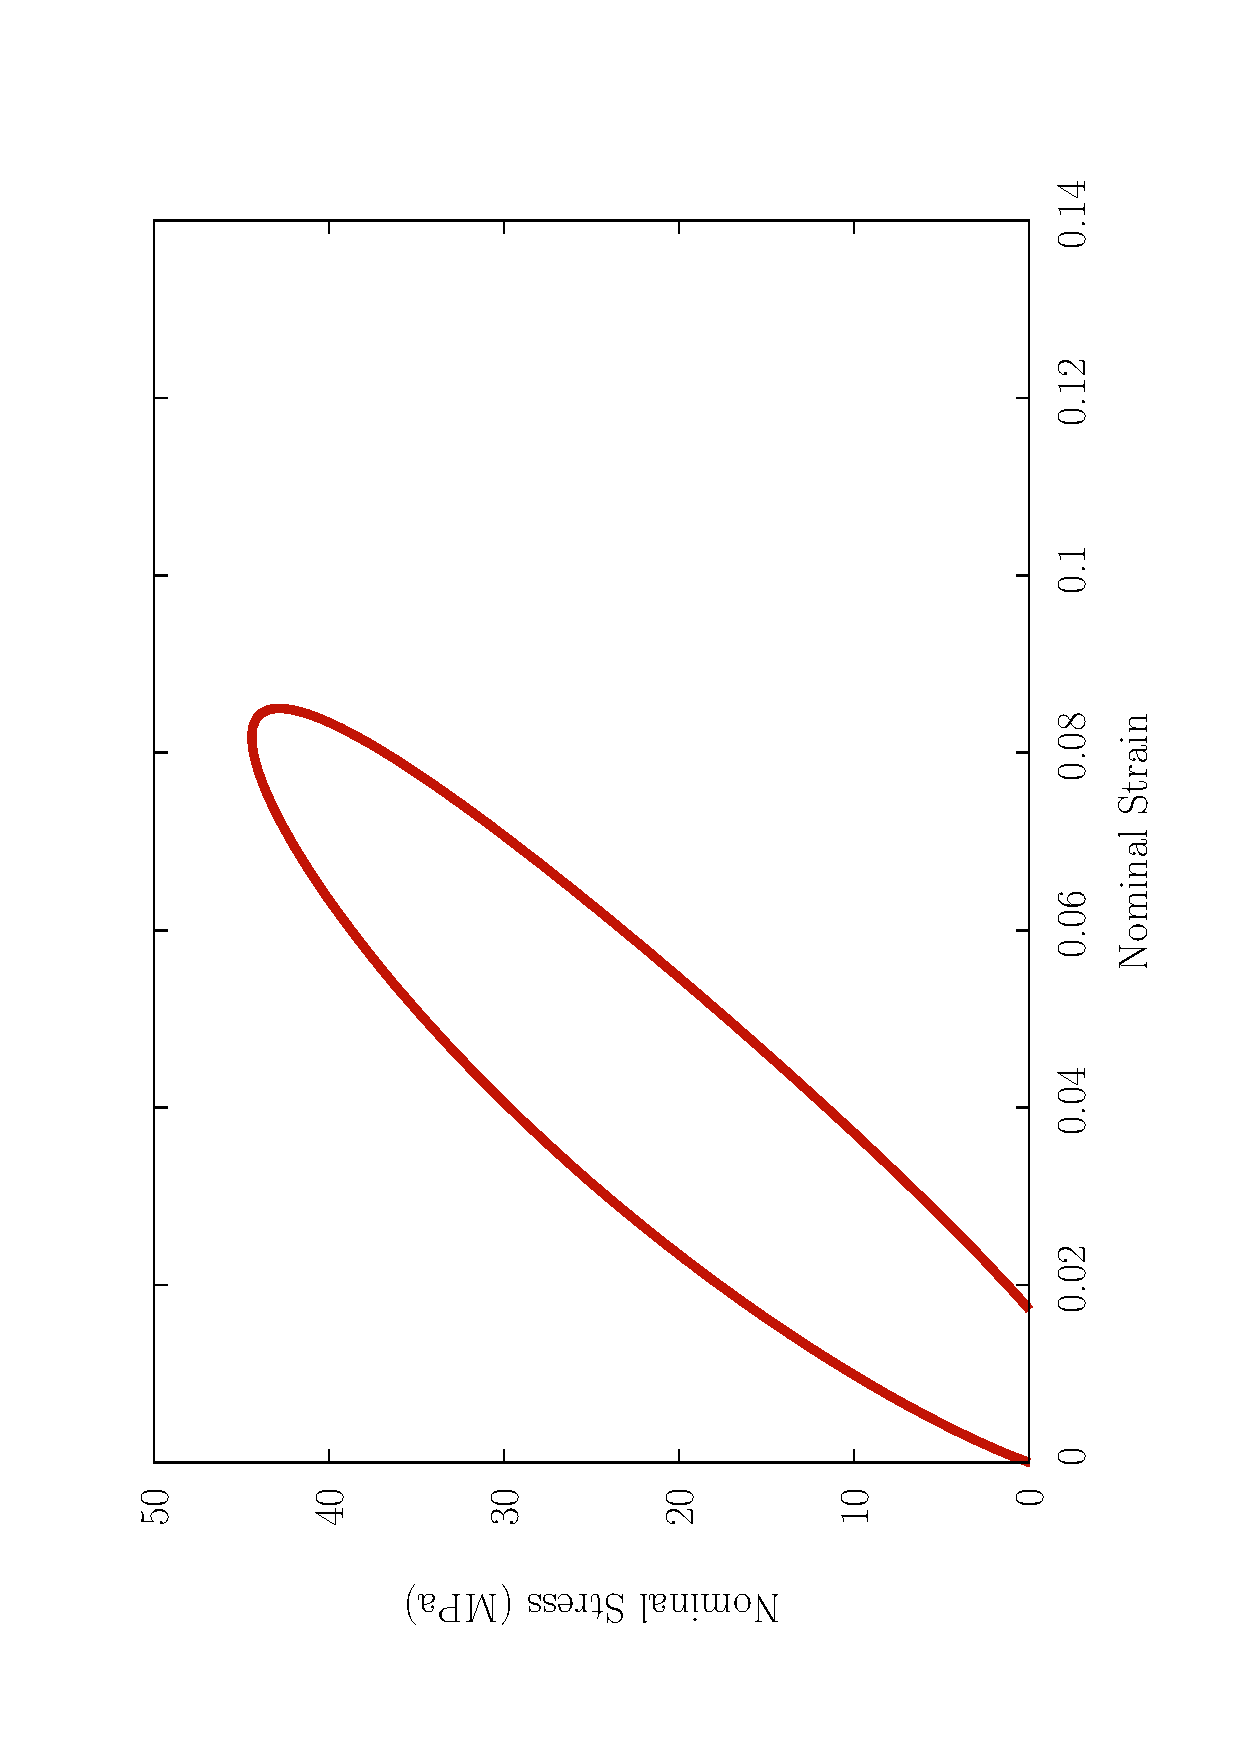
\includegraphics[width=0.6\textwidth,angle=270]{images/examples/%
eulerian/pulling/plots/visco-elastic/low-hysteresis-visco-0p01-t0p7}
\caption{Dynamic viscoelastic model, $\dot{\epsilon}=0.01$ Hz,
  $\tau=0.7$ s.}
\label{low-hysteresis-visco-0p01-t0p7}
\end{figure}

\clearpage

\section{Tumour growth}
\label{tumour-growth}

\textbullet\ Introduce the general lack of direct experimental
backing here. And point to the fact that the example will be gradually
built up from scratch to separate effects.

\subsection{Isotropic swelling}
\label{tumour-isotropic-swelling}

\textbullet\ One of the primary focuses of this work is growth, and this includes
kinematic swelling. Try to clarify that the cell concentration is
uniform, and growth is of the collagen network + cells. As a result of
this uniform cell concentration and growth, the solid tends to swell.

\textbullet\ The plots show the radial displacements at two times, and
the evolution of the area.

\begin{figure}[!hptb]
\centering
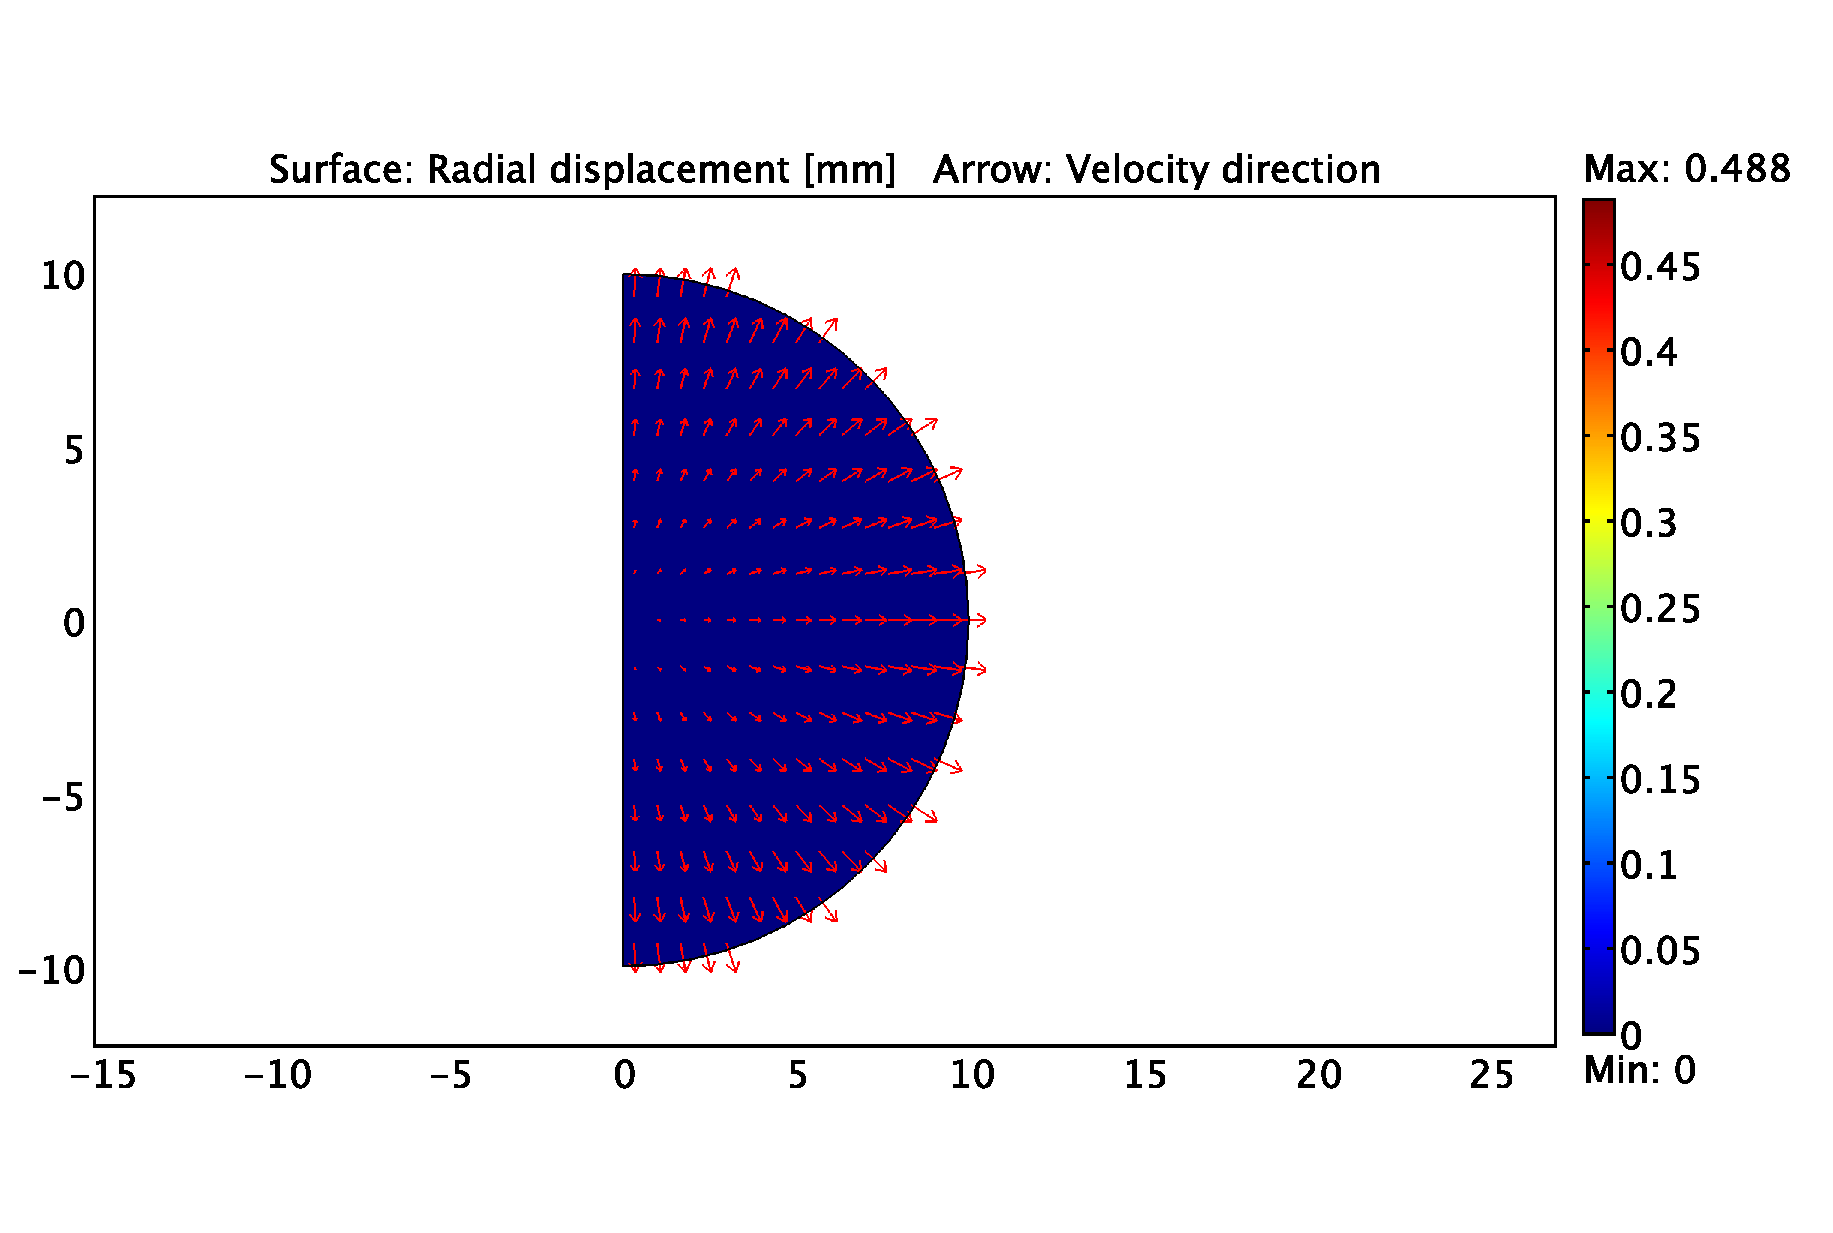
\includegraphics[width=0.8\textwidth]{images/examples/%
eulerian/cancer/isotropic-swelling-0}
\caption{A semicircular tumour at time $t=0$ days.}
\label{tumour-isotropic-swelling-0}
\end{figure}

\begin{figure}[!hptb]
\centering
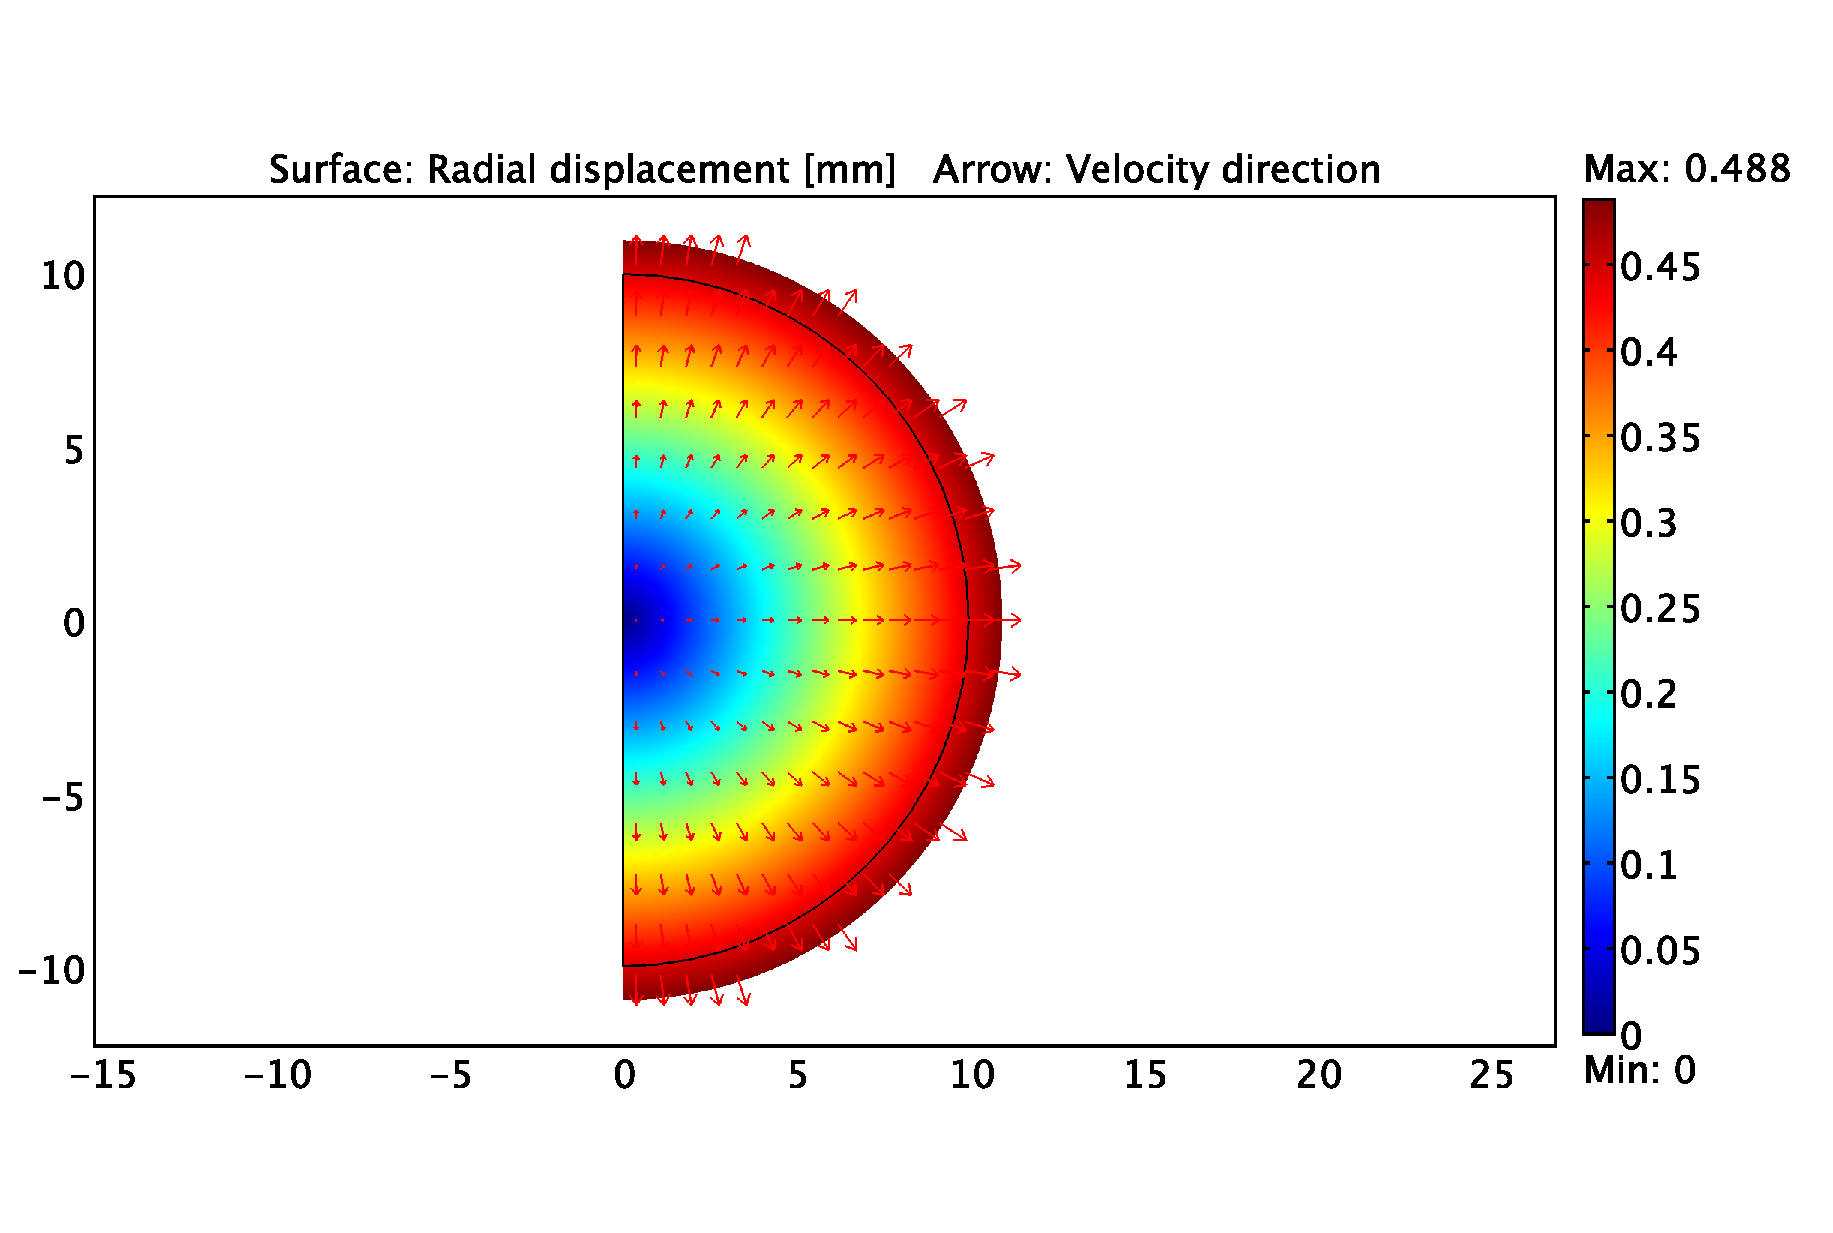
\includegraphics[width=0.8\textwidth]{images/examples/%
eulerian/cancer/isotropic-swelling-100}
\caption{A semicircular tumour at time $t=100$ days.}
\label{tumour-isotropic-swelling-100}
\end{figure}

\begin{figure}[!hptb]
\centering
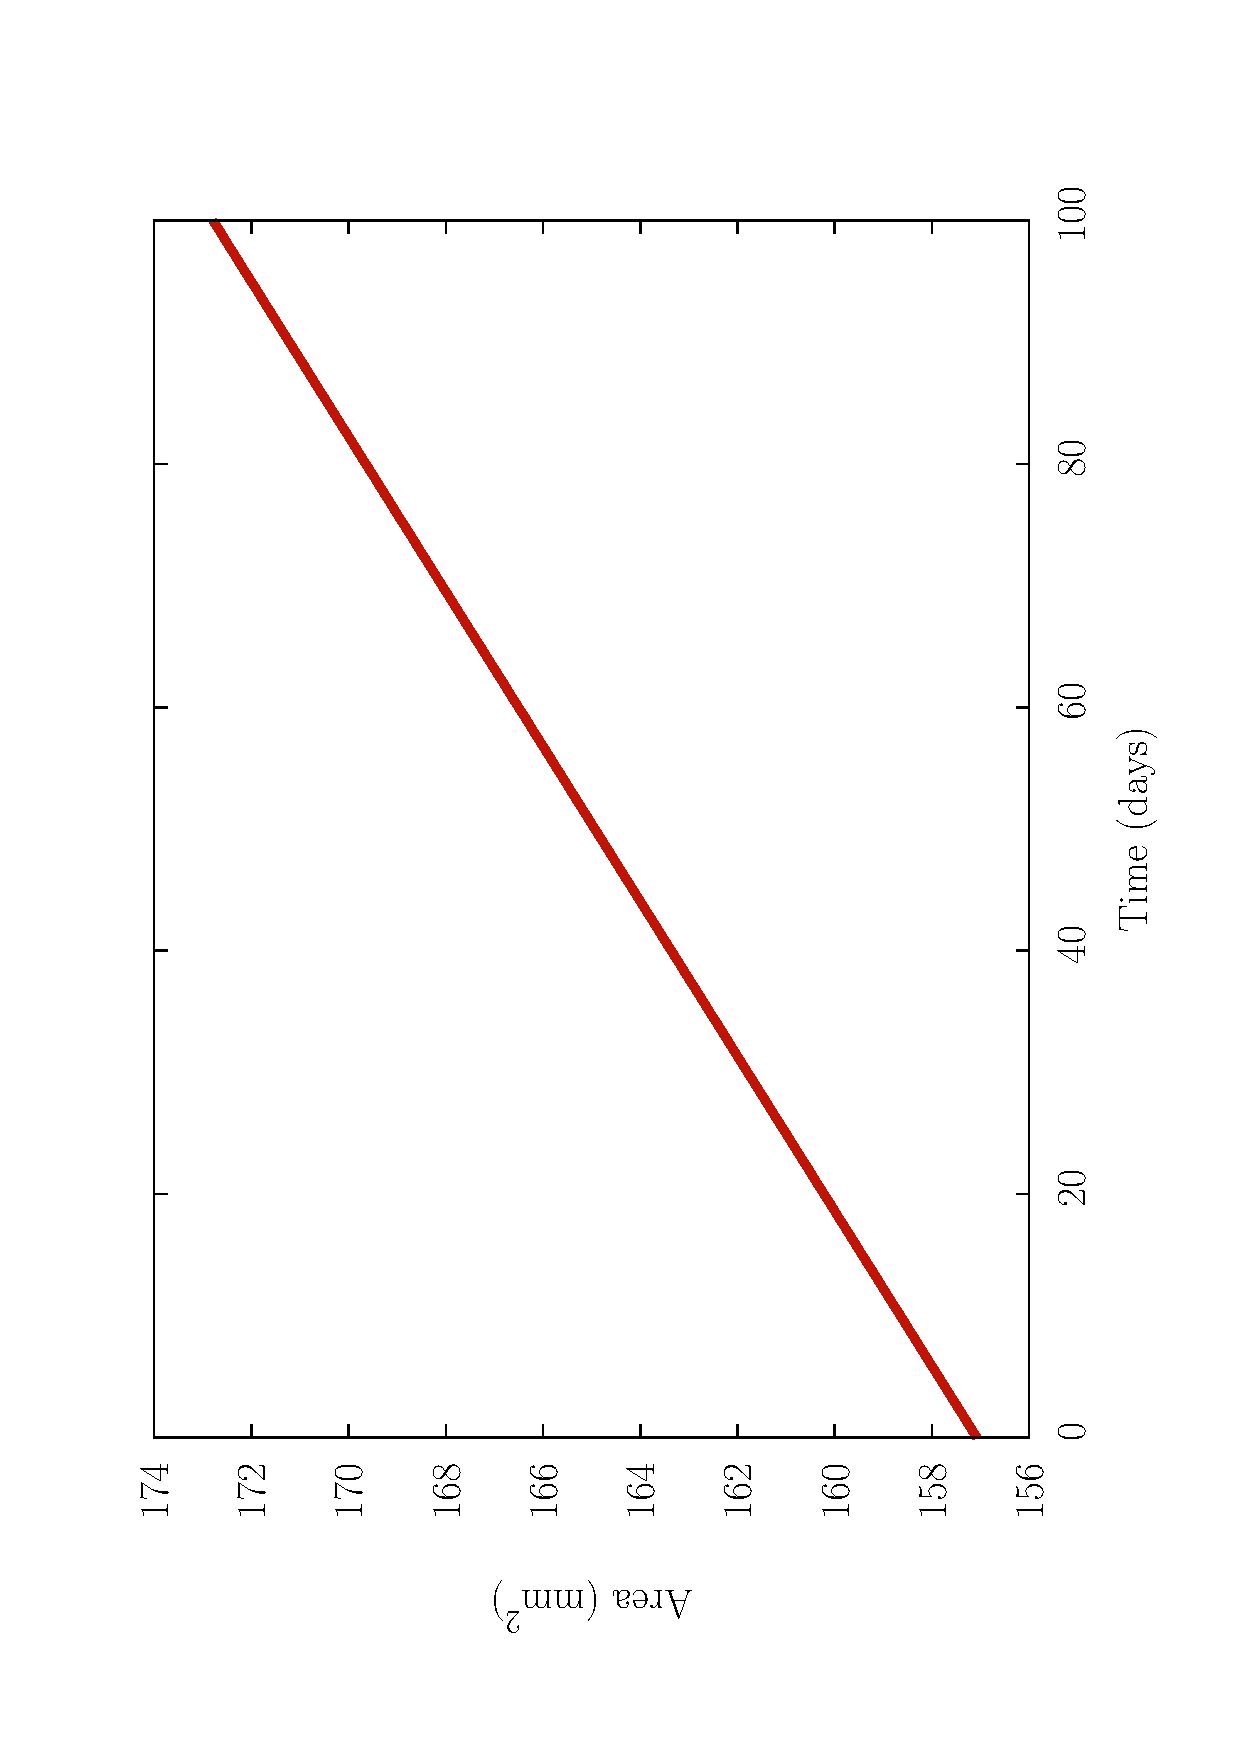
\includegraphics[width=0.6\textwidth,angle=270]{images/examples/%
eulerian/cancer/isotropic-swelling-area-evolution}
\caption{The area of the tumour evolving over 100 days.}
\label{tumour-isotropic-area-evolution}
\end{figure}

\clearpage

\subsection{Constrained by a wall}
\label{wall-constraint}

\textbullet\ Now, we're interested in the case where there is a boundary condition
arising from a wall or pressure of some sort, and since we're working
with a dynamic calculation, arbitrary introduction of the wall at some
time is numerically bad. So, we move to soft contact mechanics and
have an exponential rule like so that kicks in gradually. The cells
still don't do any mechanics, yet.

\textbullet\ The plot shows the velocity of the growing tumour
(arrows) and the compressive horizontal stress built up at a certain
time. Notice that the velocity in those regions are zeroing out, as
they should. The temporal variation at that end point is plotted separately.

\begin{figure}[!hptb]
\centering
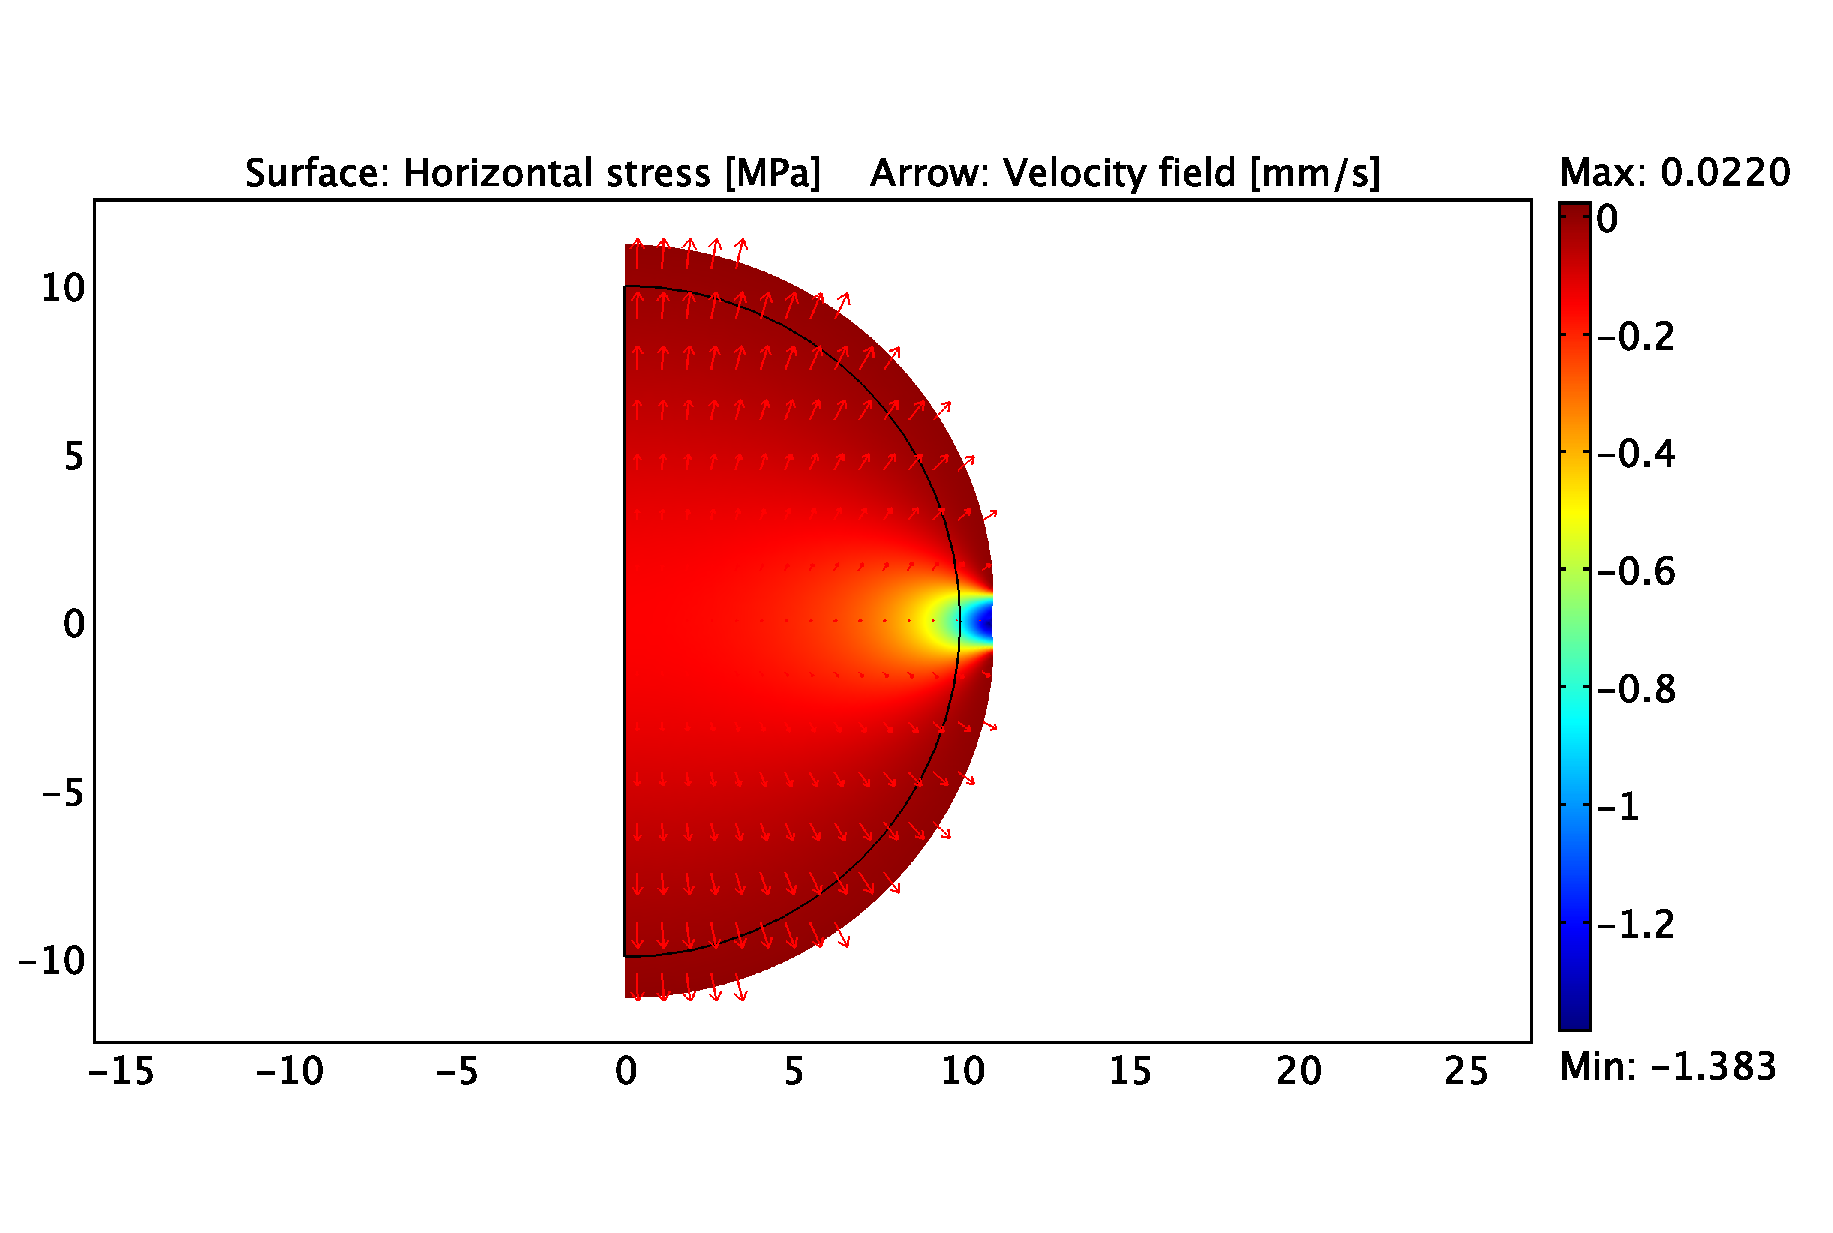
\includegraphics[width=0.8\textwidth]{images/examples/%
eulerian/cancer/constrained-swelling-120}
\caption{The growing tumour constrained by a wall at time $t=100$ days.}
\label{tumour-constrained-swelling-120}
\end{figure}

\begin{figure}[!hptb]
\centering
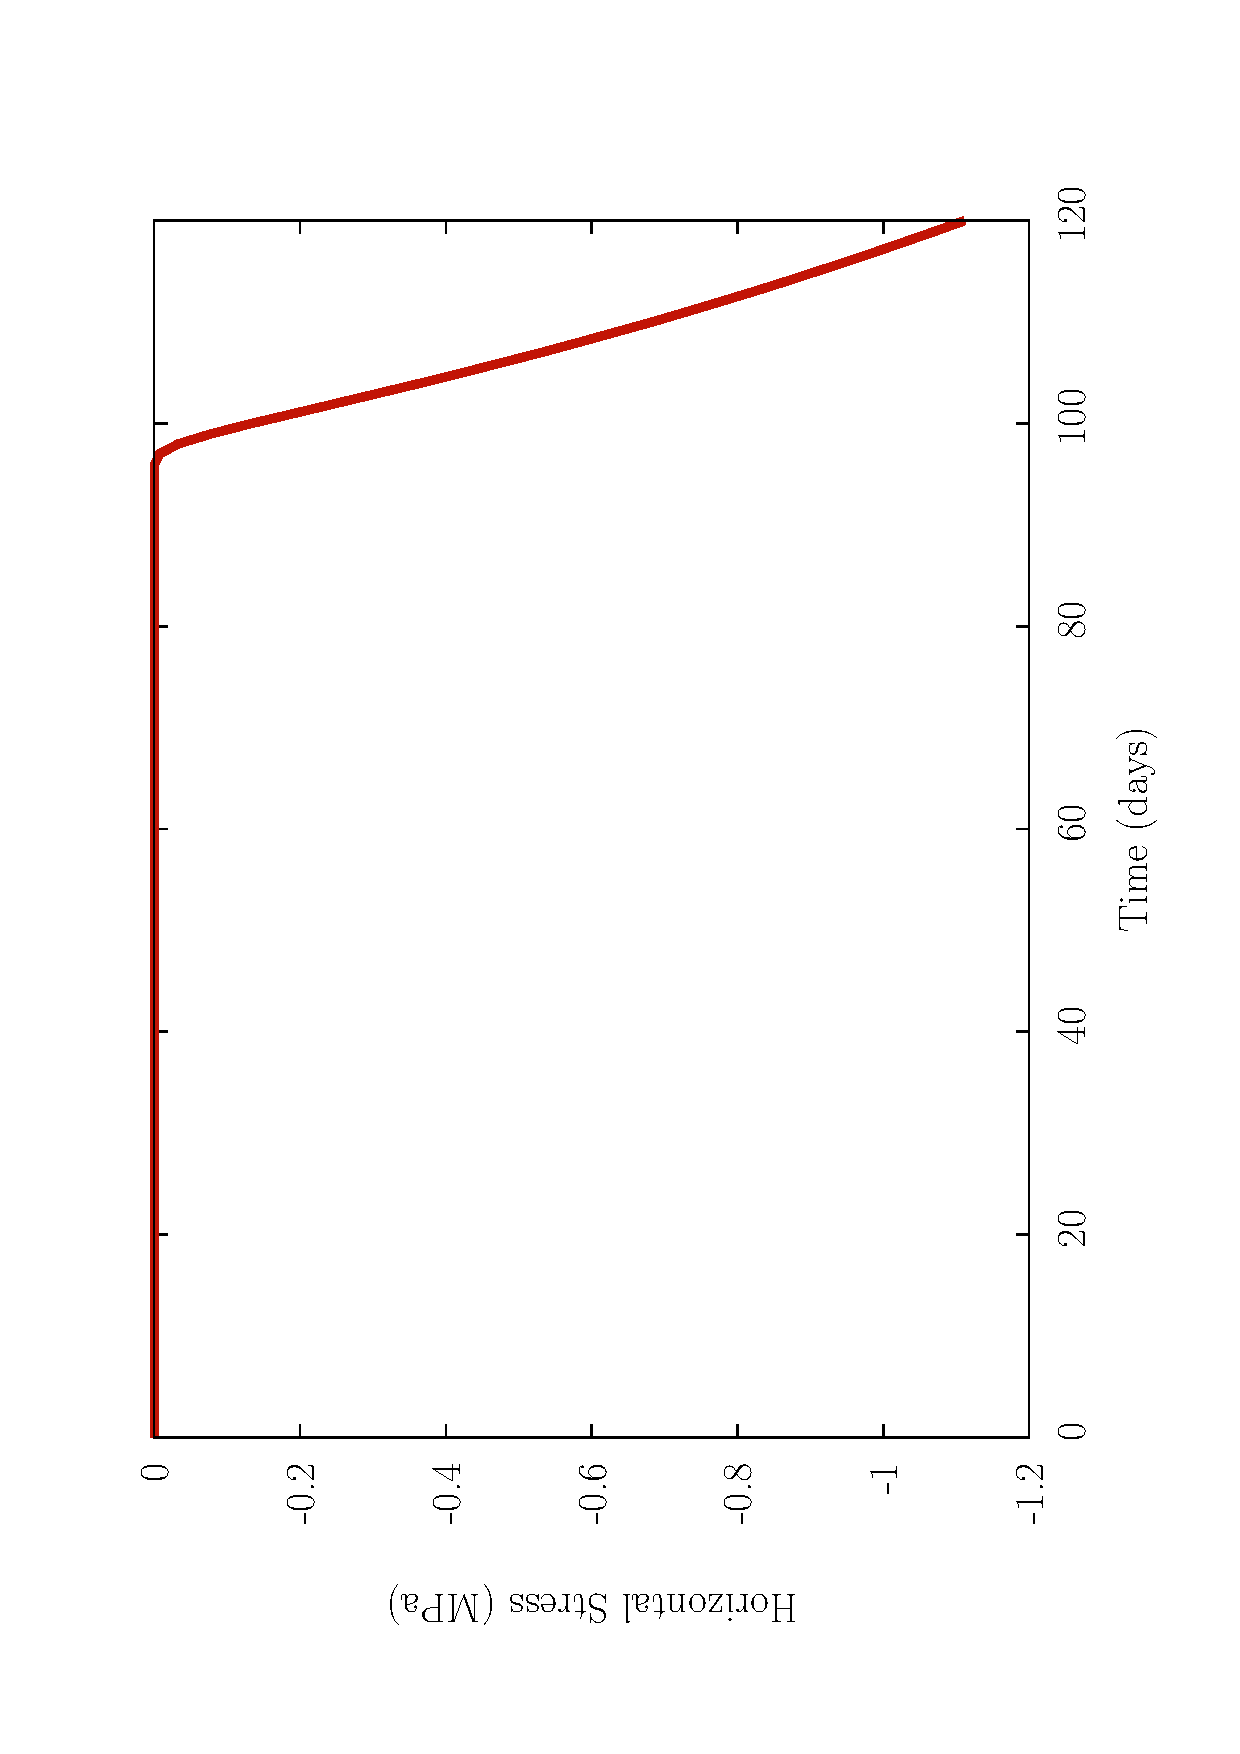
\includegraphics[width=0.6\textwidth,angle=270]{images/examples/%
eulerian/cancer/constrained-stress-evolution}
\caption{The horizontal stress in the tumour evolving over 120 days.}
\label{tumour-constrained-stress-evolution}
\end{figure}

\subsection{The mechanics of cells}
\label{cell-roles}

So far, we worked with no mechanics but there are two fundamental
things cells do.

\subsubsection{Inward tug}
\label{inward-tug}

\textbullet\ Cells pull inwards, following this law that says that an
optimal cell-ECM concentration is best for maximum inward
tuginess. Their stress now follows this rule motivated by this paper.

\textbullet\ As a result of uniform cell concentrations, we see
this. As a result of an (arbitrary) heterogeneous contribution, we see
something else. Note that the regions with higher cells pull in more.

\begin{figure}[!hptb]
\centering
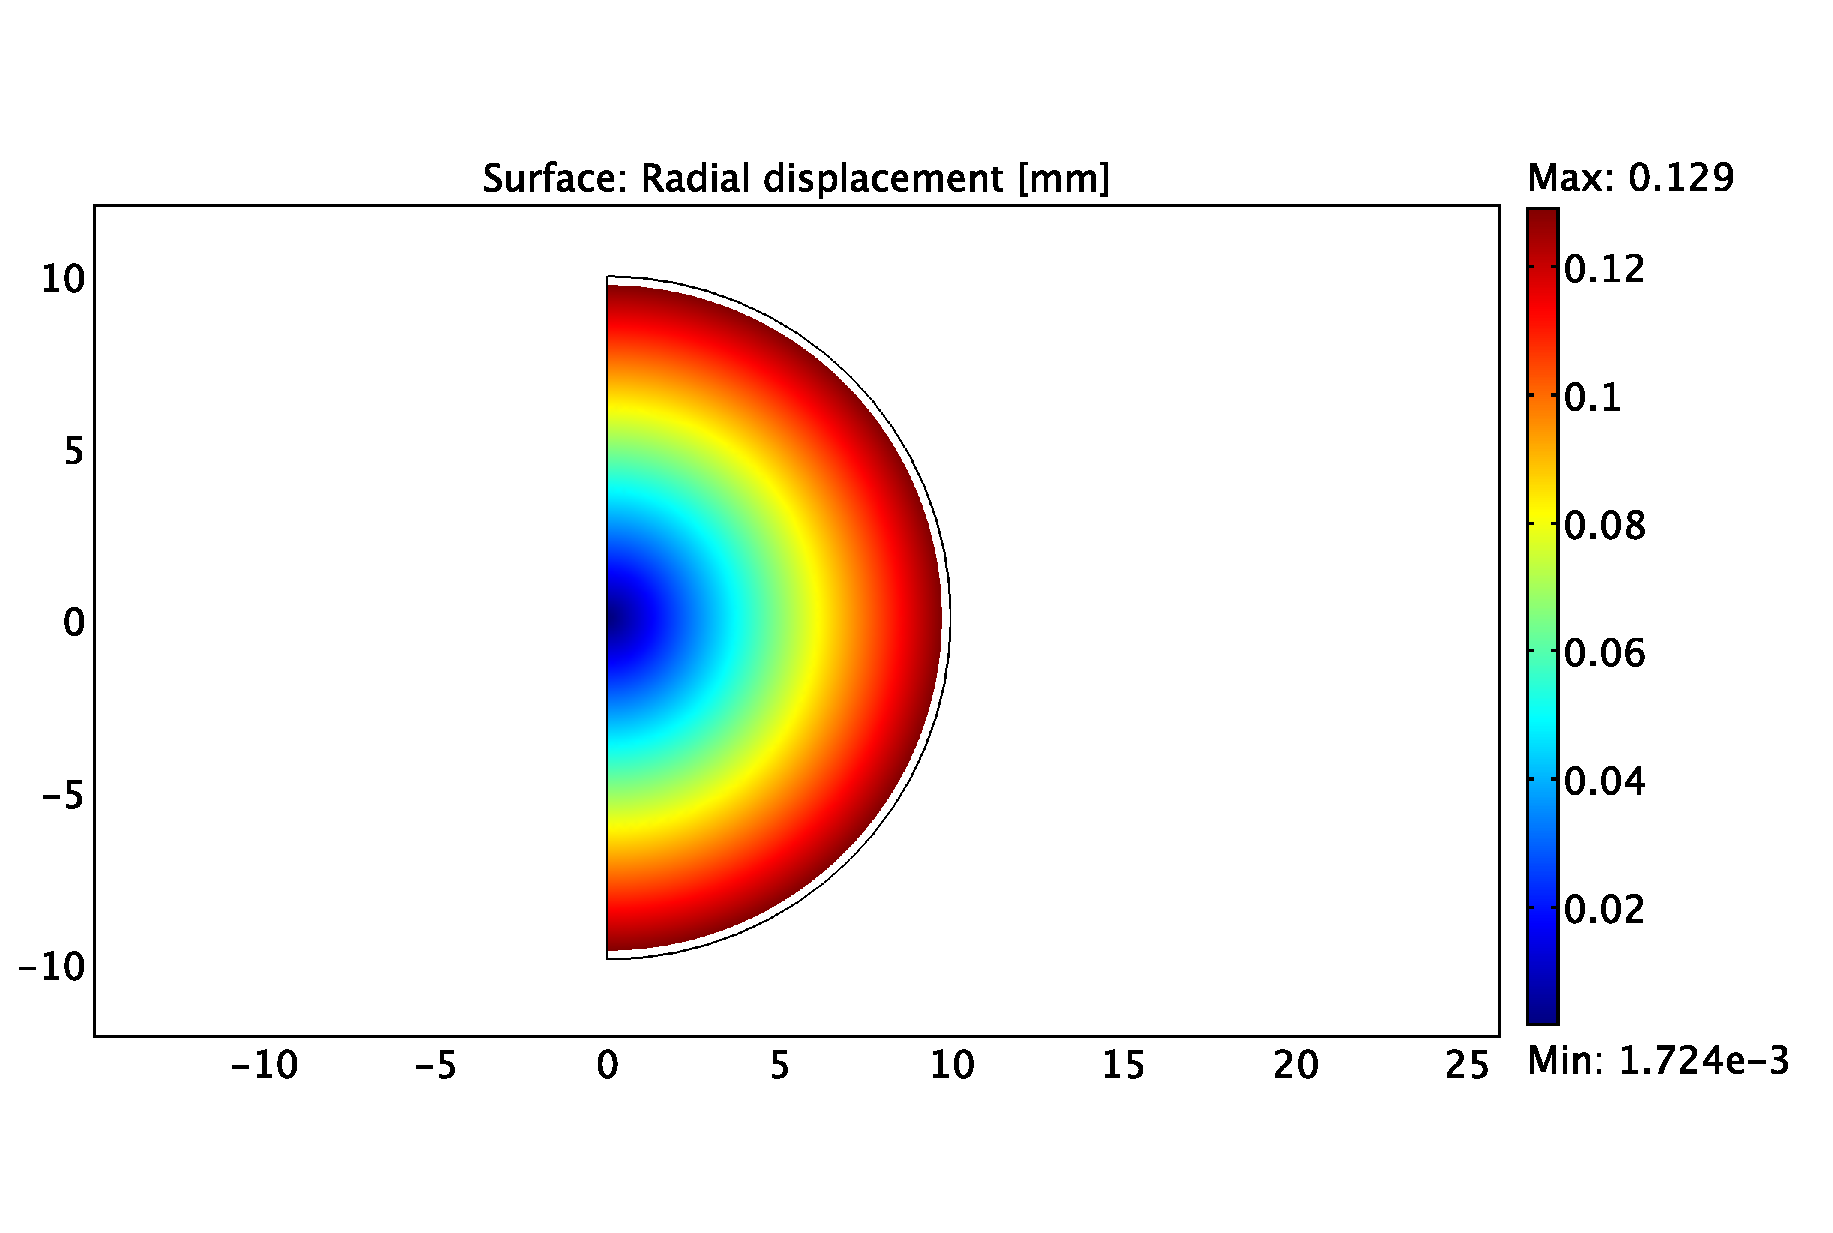
\includegraphics[width=0.8\textwidth]{images/examples/%
eulerian/cancer/homogeneous-inward-tug}
\caption{Homogeneous inward tug due to a uniform distribution of cells.}
\label{tumour-homogeneous-inward-tug}
\end{figure}

\begin{figure}[!hptb]
\centering
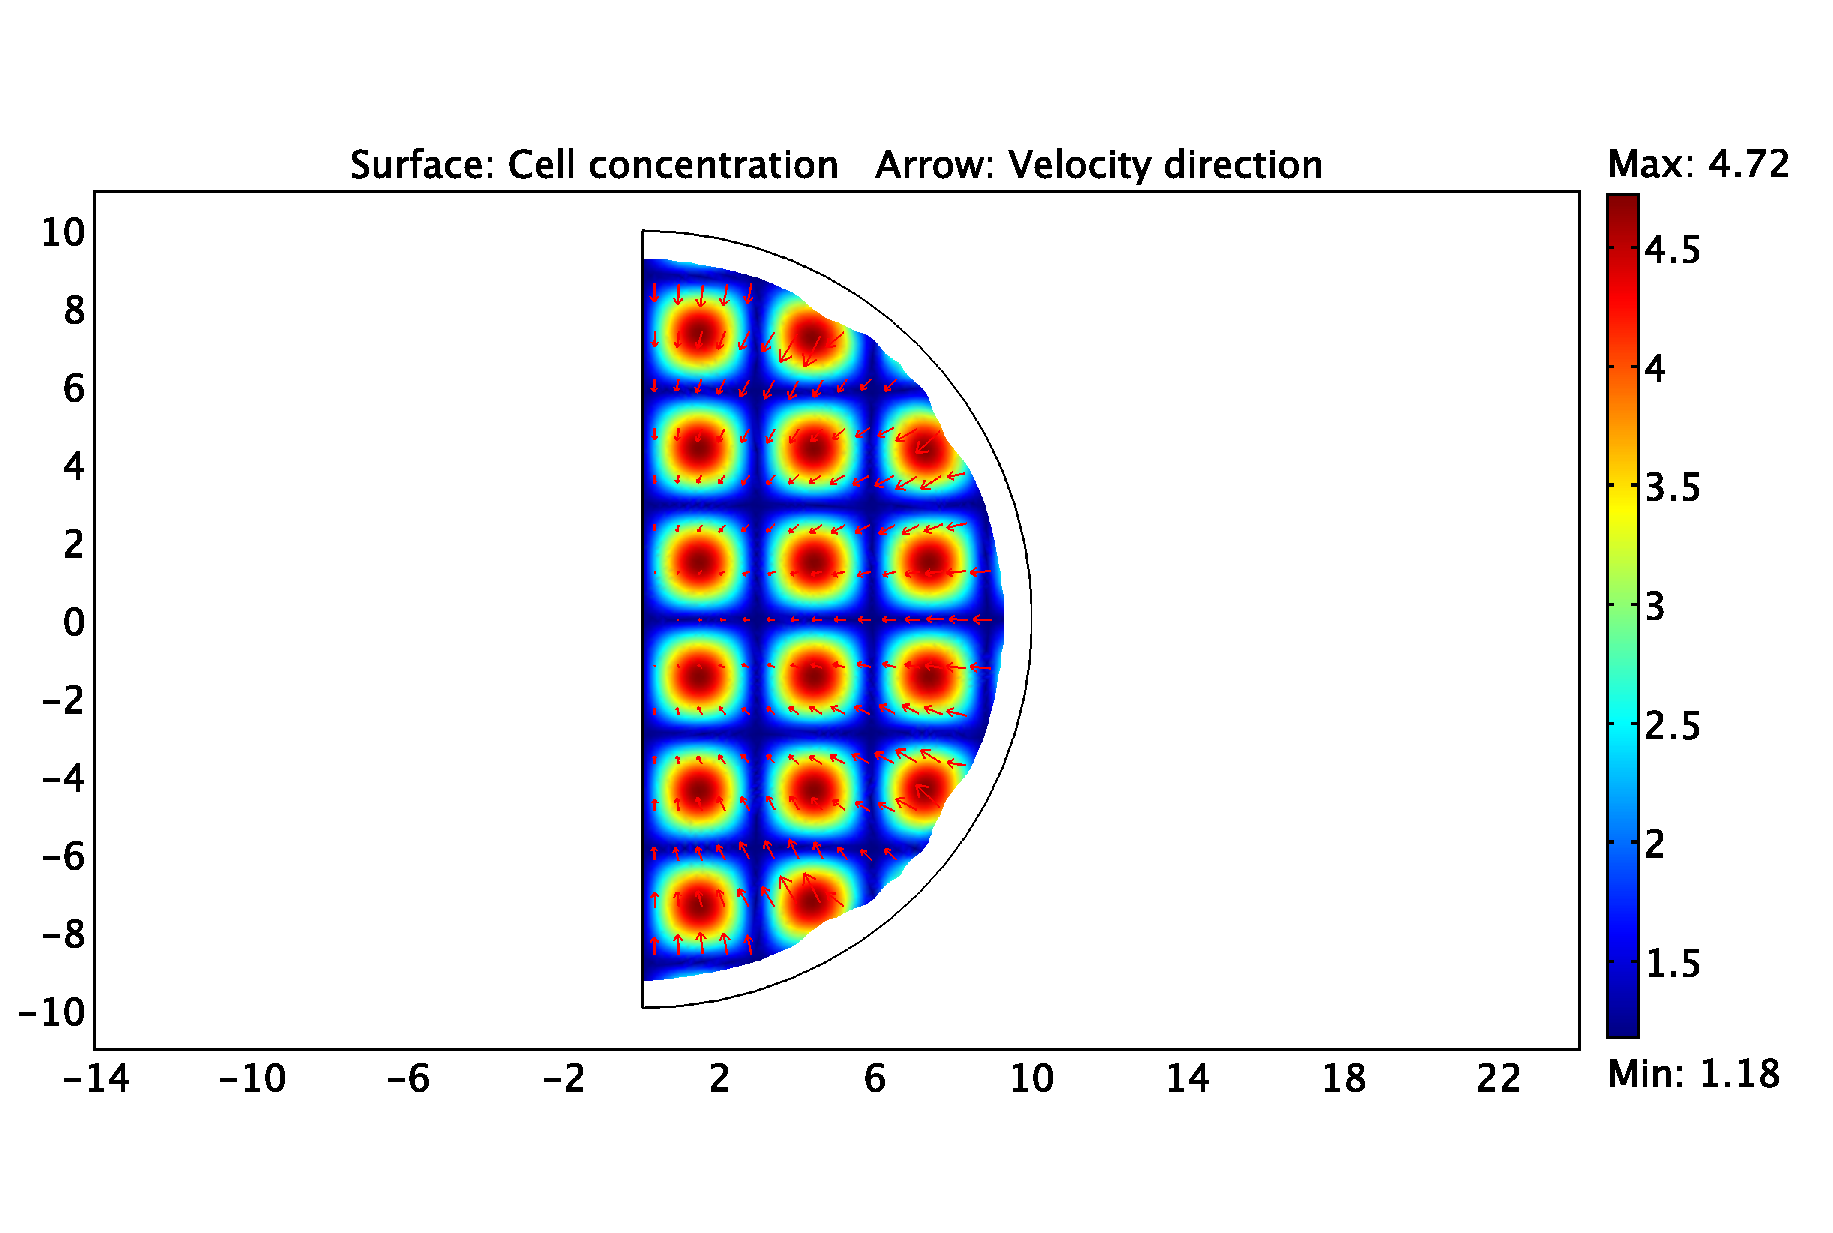
\includegraphics[width=0.8\textwidth]{images/examples/%
eulerian/cancer/heterogeneous-inward-tug}
\caption{Heterogeneous inward tug due to a non-uniform distribution of cells.}
\label{tumour-heterogeneous-inward-tug}
\end{figure}

\clearpage

\subsubsection{Transport of the cells}
\label{cell-transport}

\textbullet\ So far, we assumed that the cell concentration remains
constant in time and space. Now we add an additional differential
equation (advection diffusion reaction governing its
movement). Diffusion is obvious, and the plots below show the cells
diffusing from a central bulb outwards while they proliferate.

{\bf Diffusion and proliferation}

\begin{figure}[!hptb]
\centering
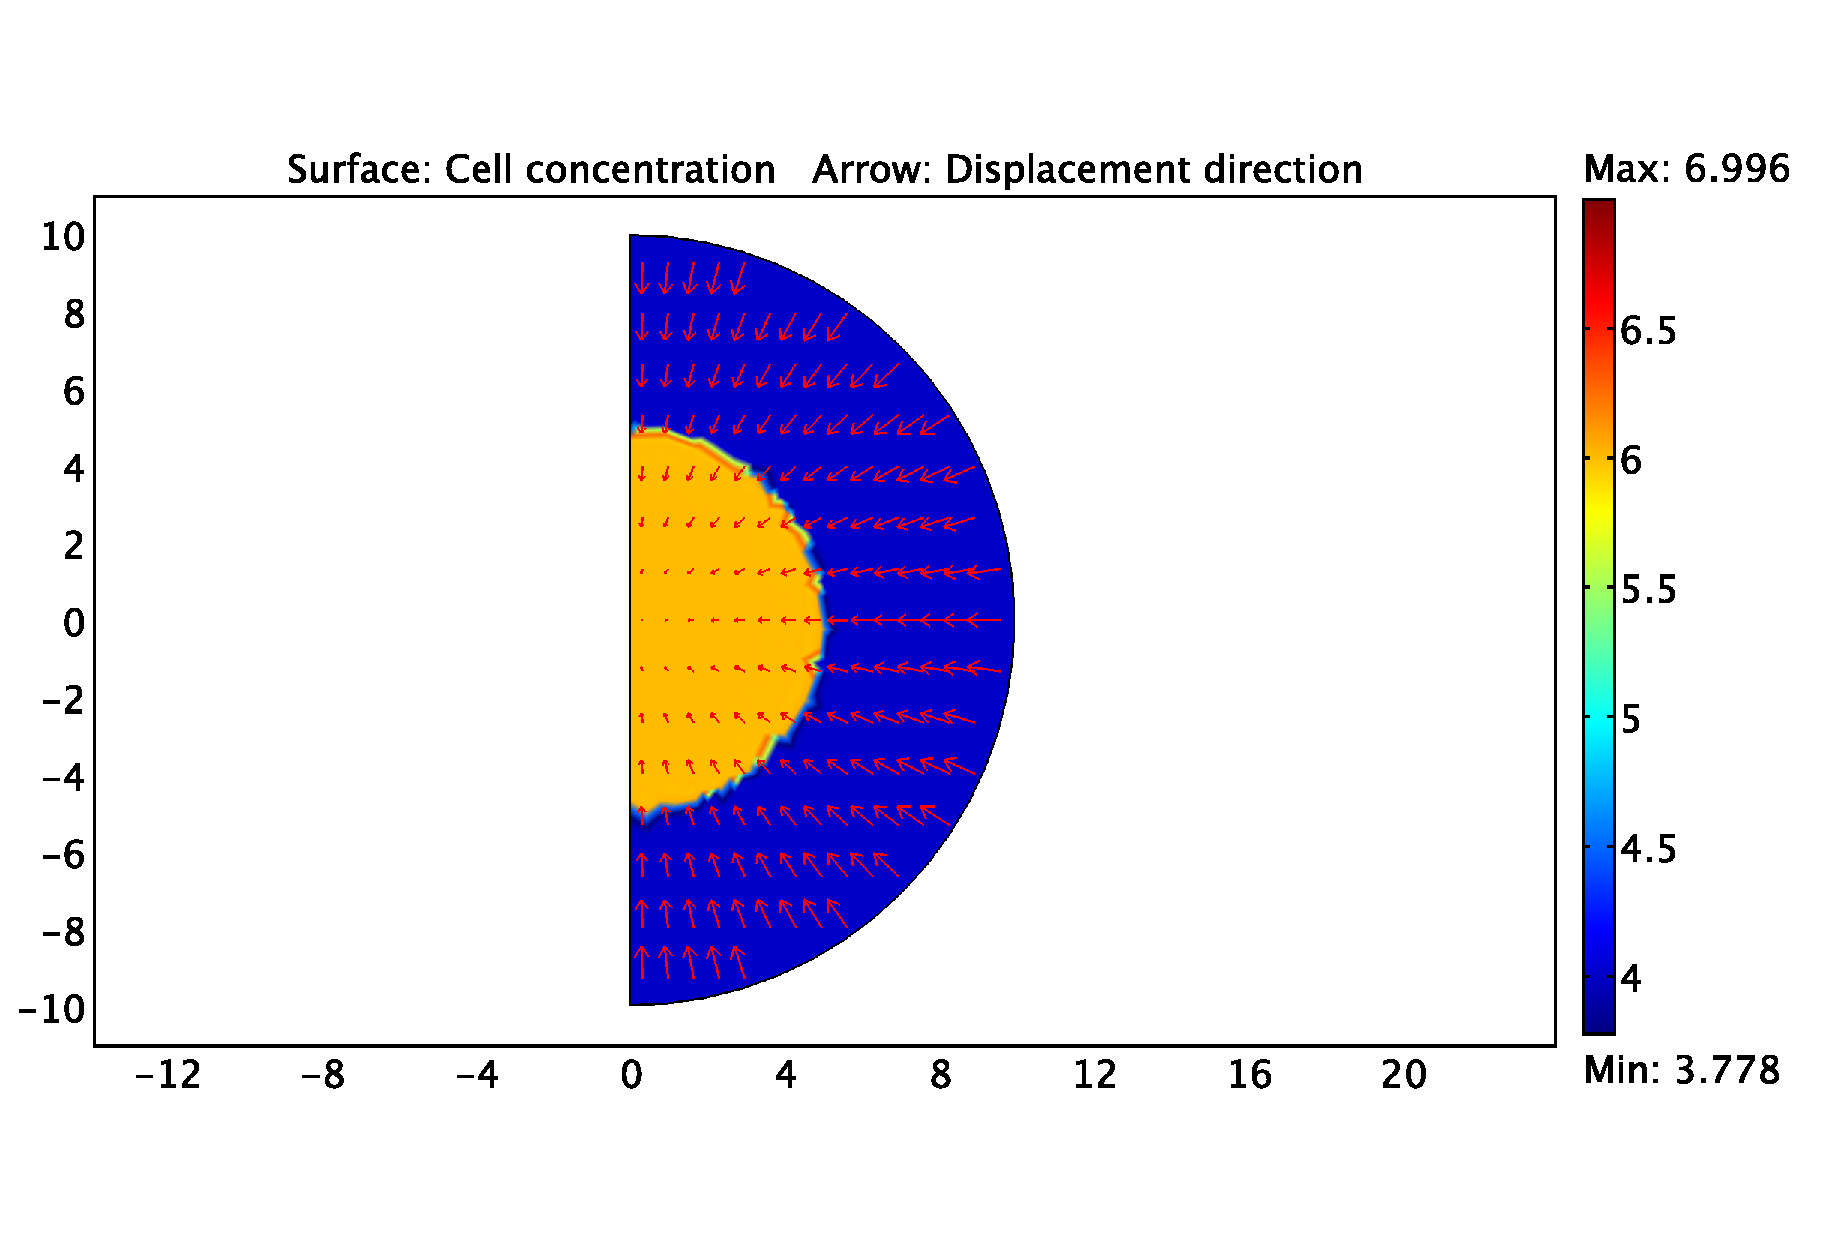
\includegraphics[width=0.8\textwidth]{images/examples/%
eulerian/cancer/diffusing-proliferating-cells-0}
\caption{The cells diffusing and proliferating at time $t=0$ days.}
\label{tumour-diffusion-proliferation-0}
\end{figure}

\begin{figure}[!hptb]
\centering
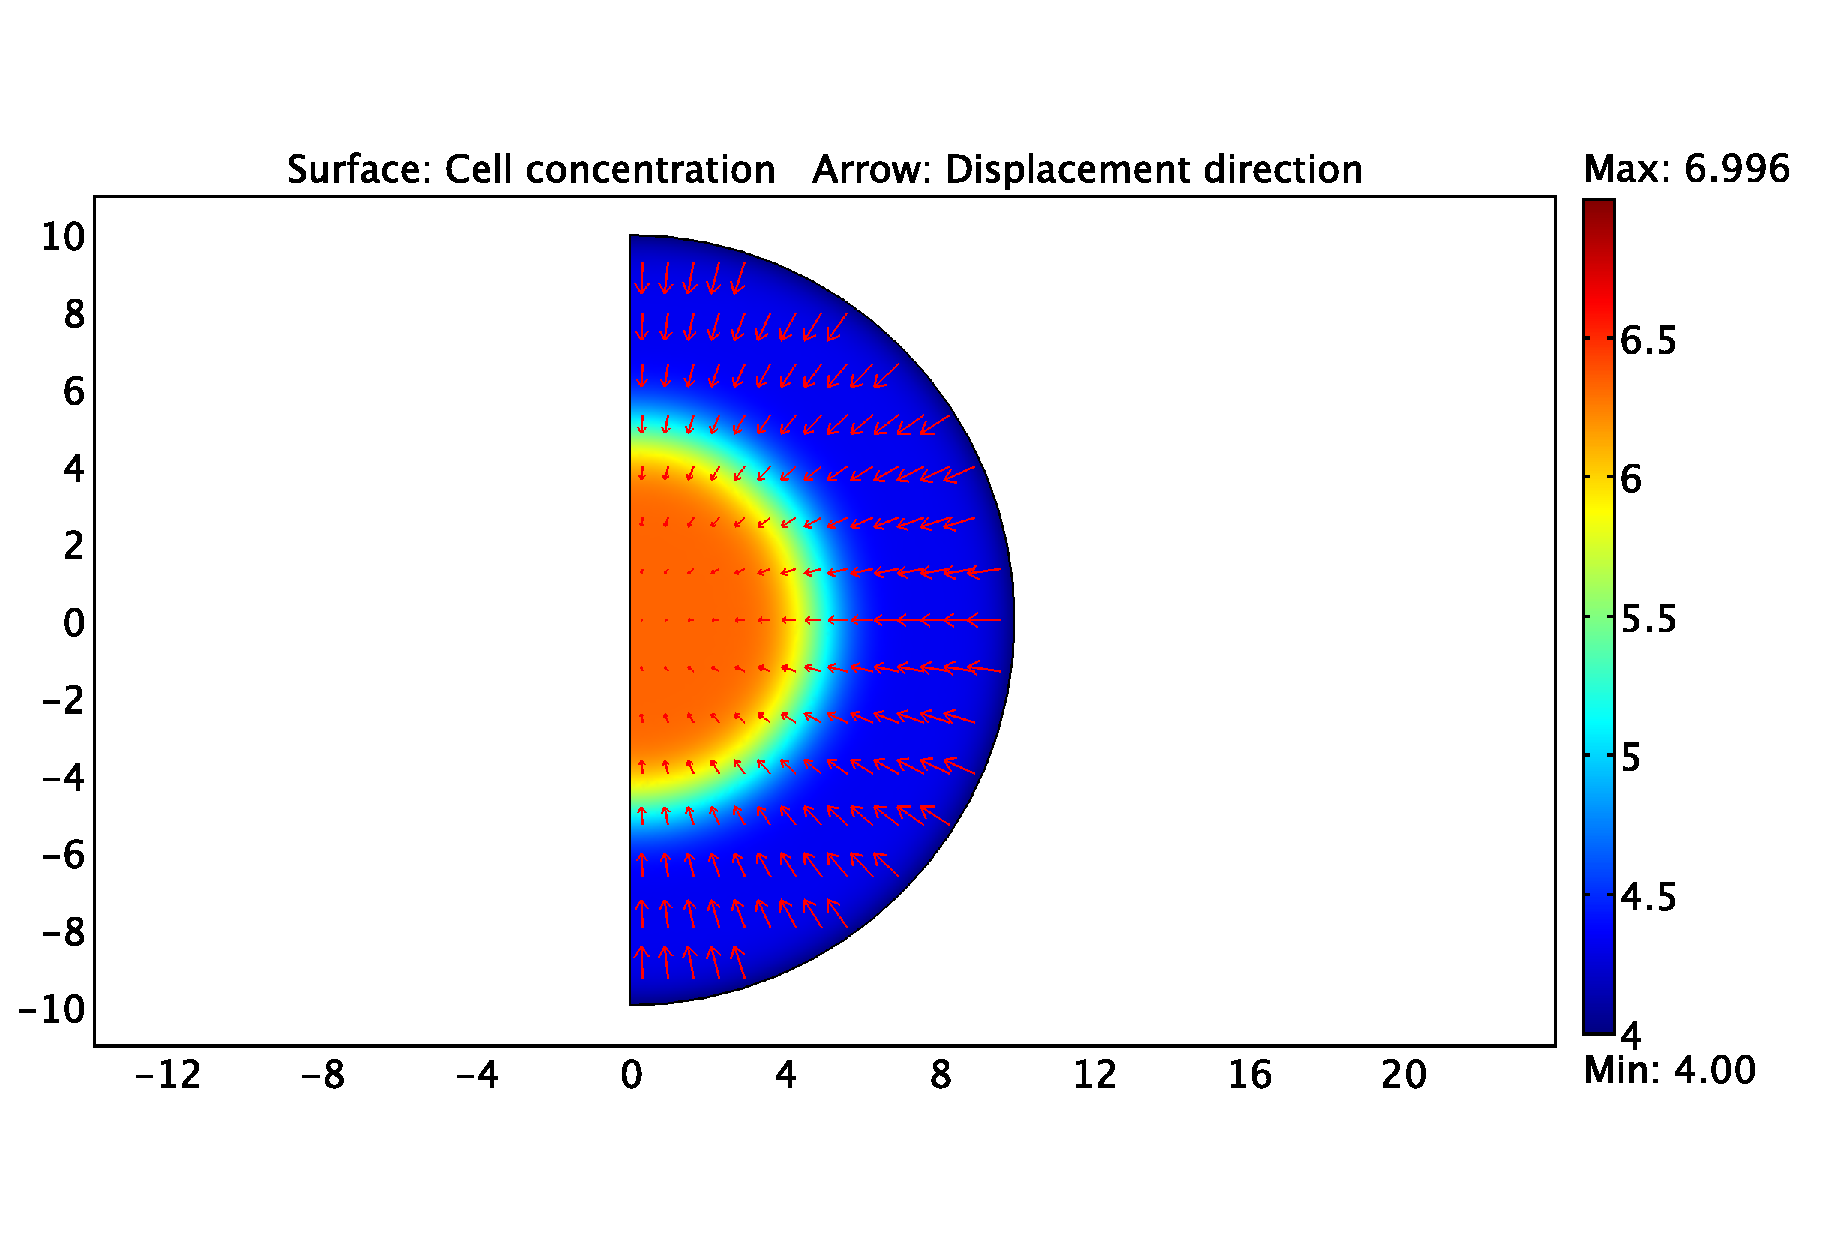
\includegraphics[width=0.8\textwidth]{images/examples/%
eulerian/cancer/diffusing-proliferating-cells-33}
\caption{The cells diffusing and proliferating at time $t=33$ days.}
\label{tumour-diffusion-proliferation-33}
\end{figure}

\begin{figure}[!hptb]
\centering
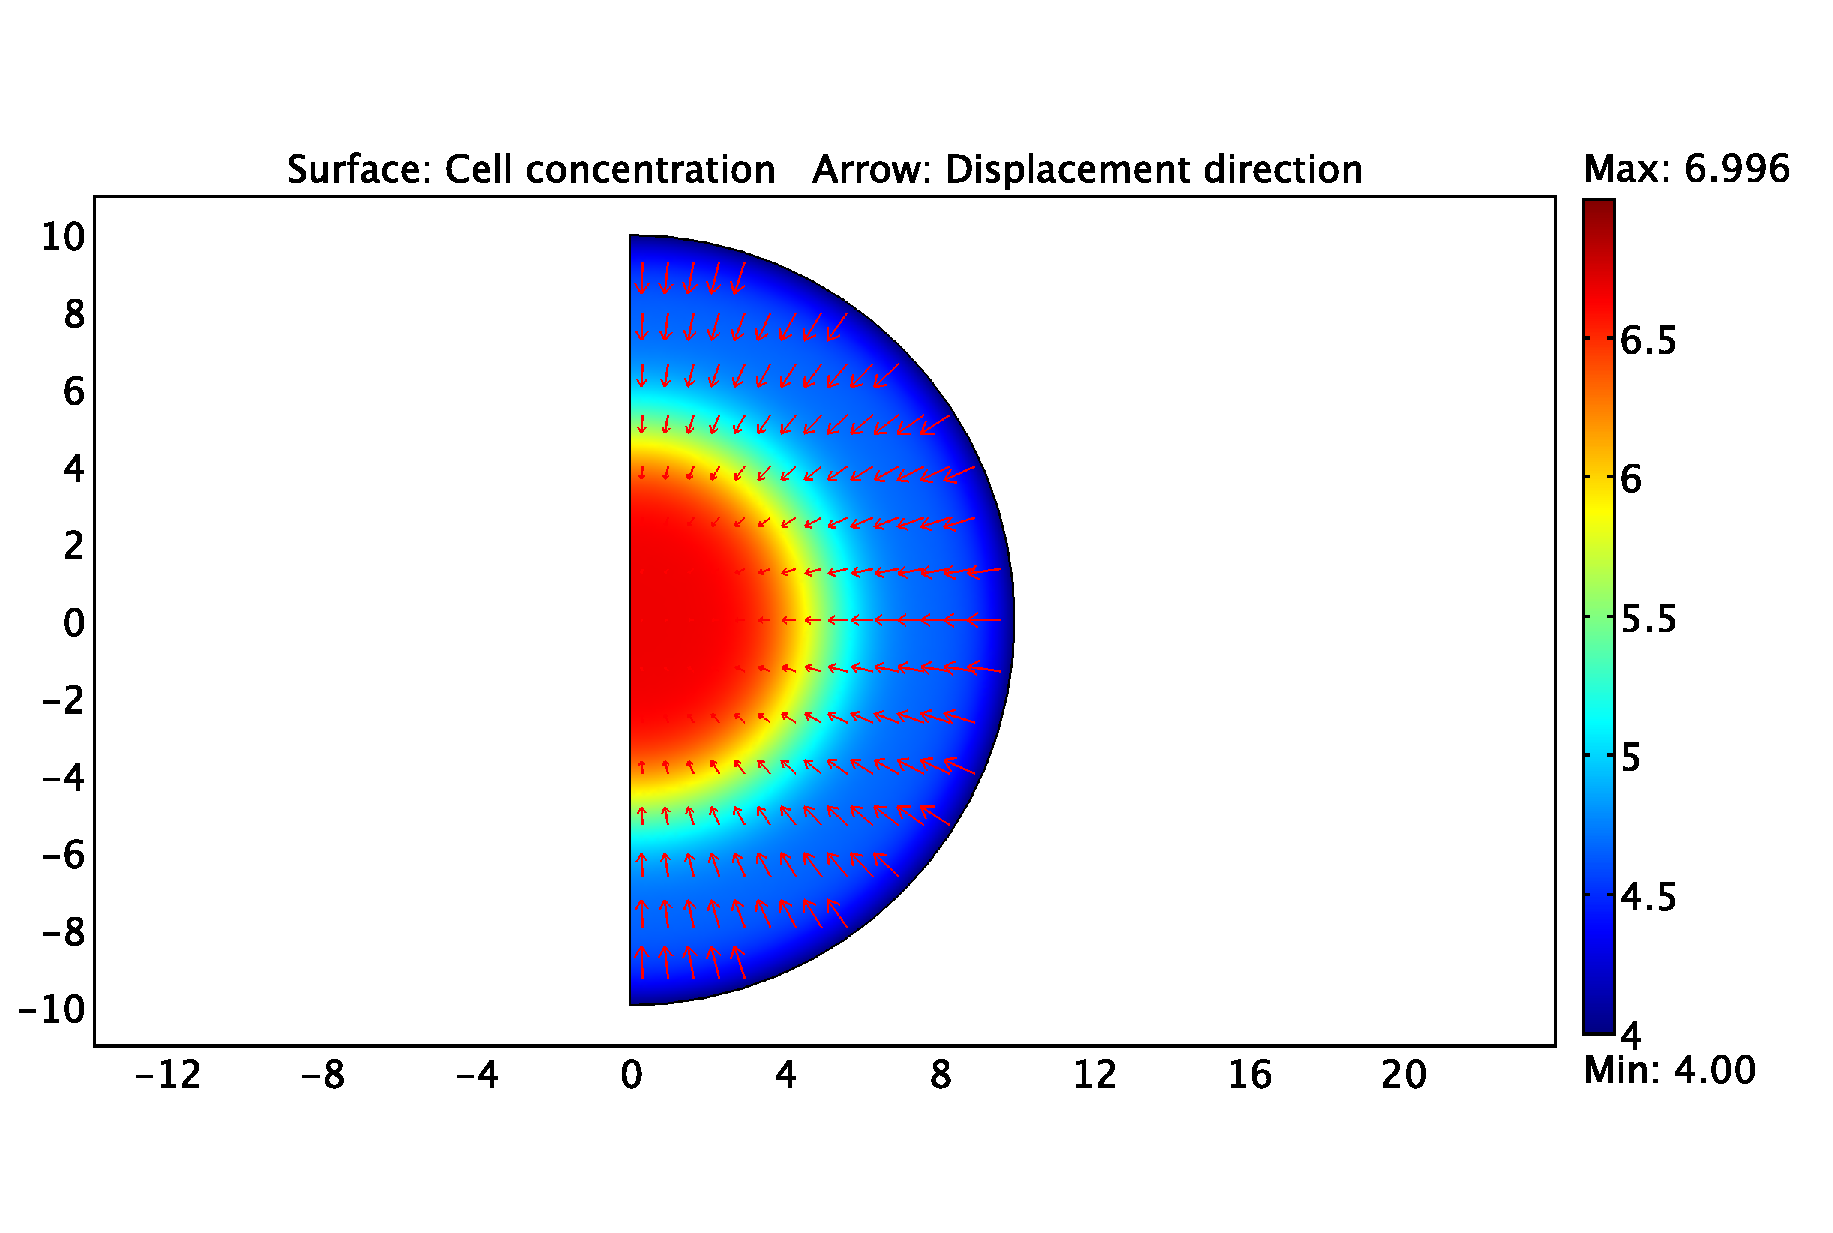
\includegraphics[width=0.8\textwidth]{images/examples/%
eulerian/cancer/diffusing-proliferating-cells-67}
\caption{The cells diffusing and proliferating at time $t=67$ days.}
\label{tumour-diffusion-proliferation-67}
\end{figure}

\begin{figure}[!hptb]
\centering
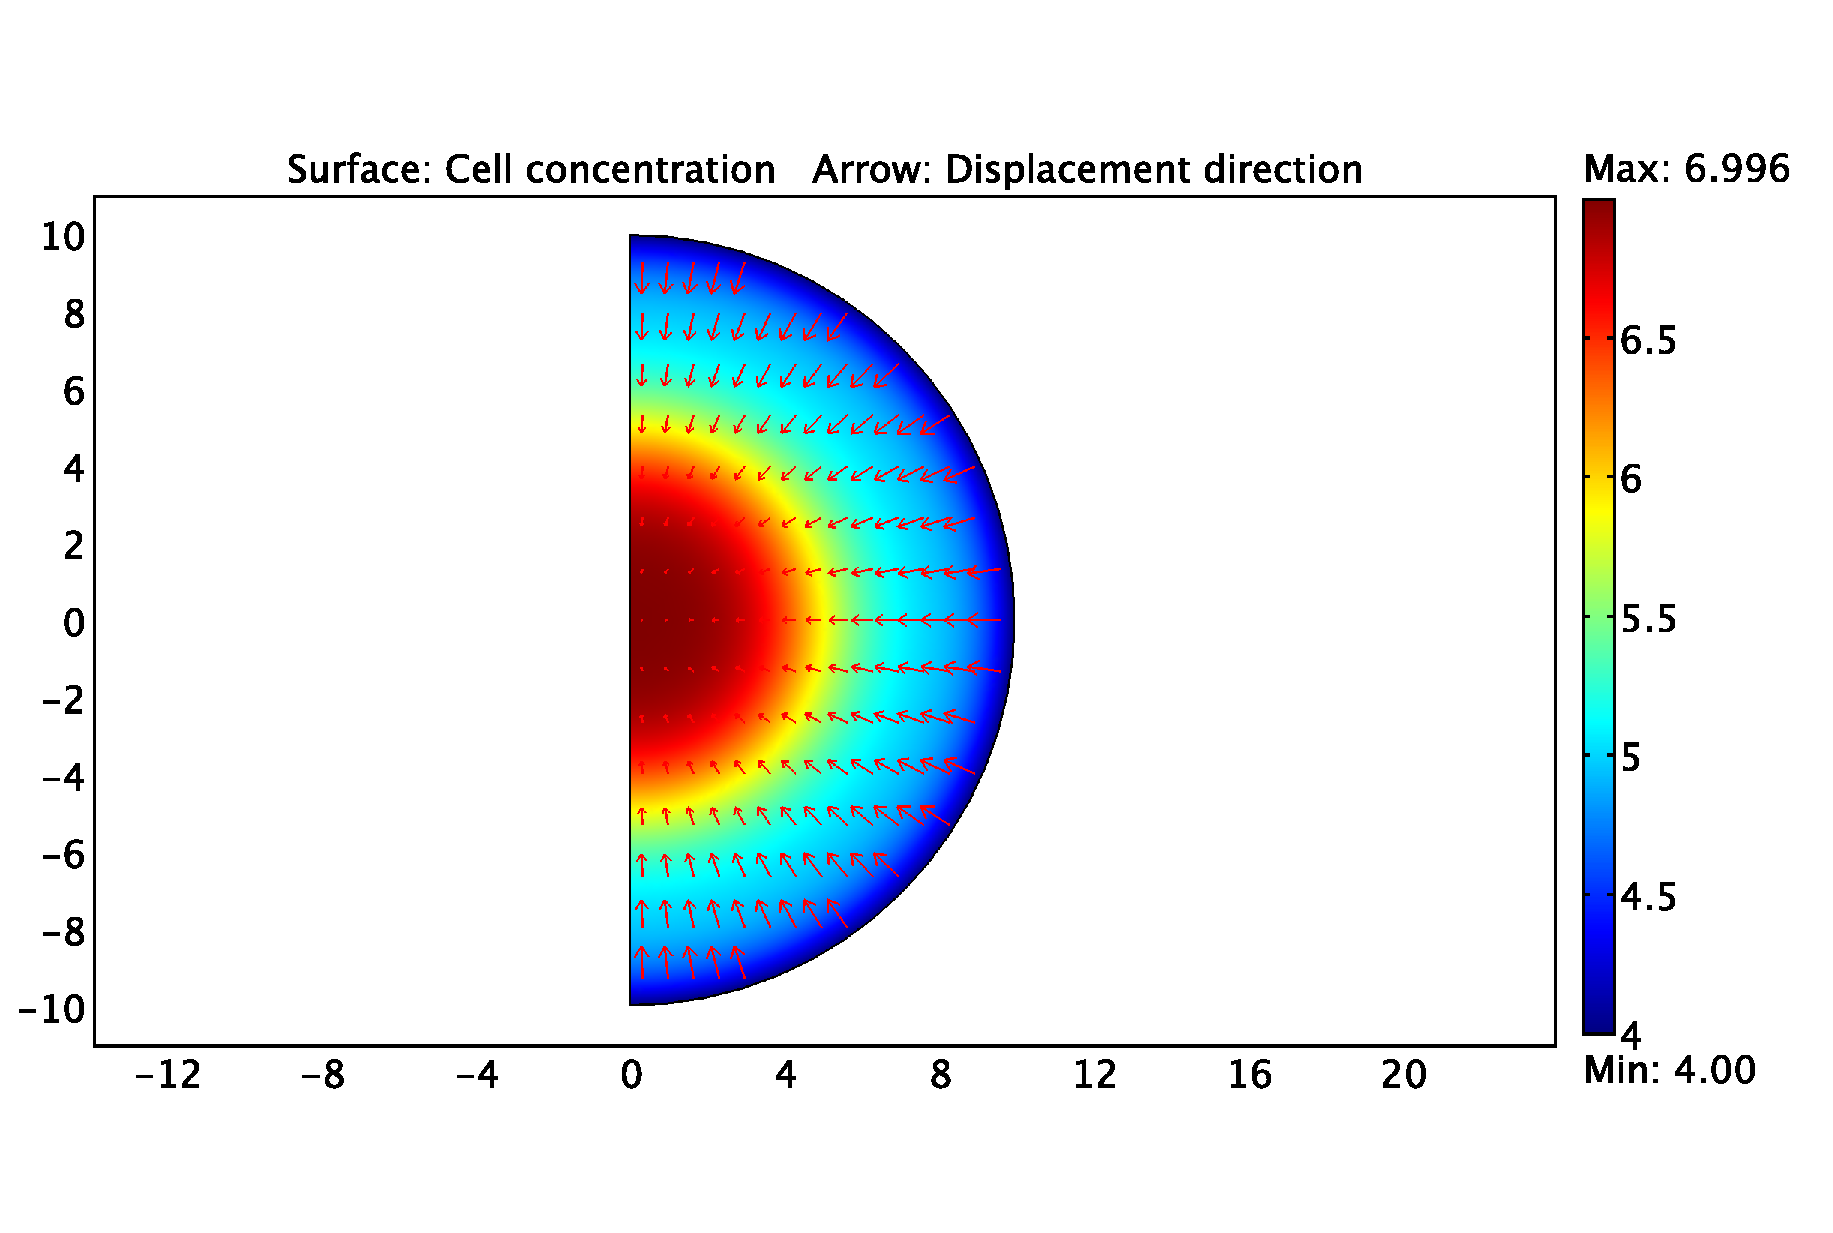
\includegraphics[width=0.8\textwidth]{images/examples/%
eulerian/cancer/diffusing-proliferating-cells-100}
\caption{The cells diffusing and proliferating at time $t=100$ days.}
\label{tumour-diffusion-proliferation-100}
\end{figure}

\subsubsection{Cell haptotaxis}
\label{eu-cell-haptotaxis}

\textbullet\ But there is another mechanism for their movement, they
move along the gradients of ECM contributions. This is added as an
additional flux term to the calculation above, and the magnitude of
this mobility is motivated by this paper. Clearly, this effect is
less/more important than general diffusion.

\textbullet\ In order to kick this off, we start with an (arbitrary)
heterogeneous ECM concentration, as shown. Note that the cell inward
tug changes with the concentration, as noted by the sizes and
directions of the arrows.

\begin{figure}[!hptb]
\centering
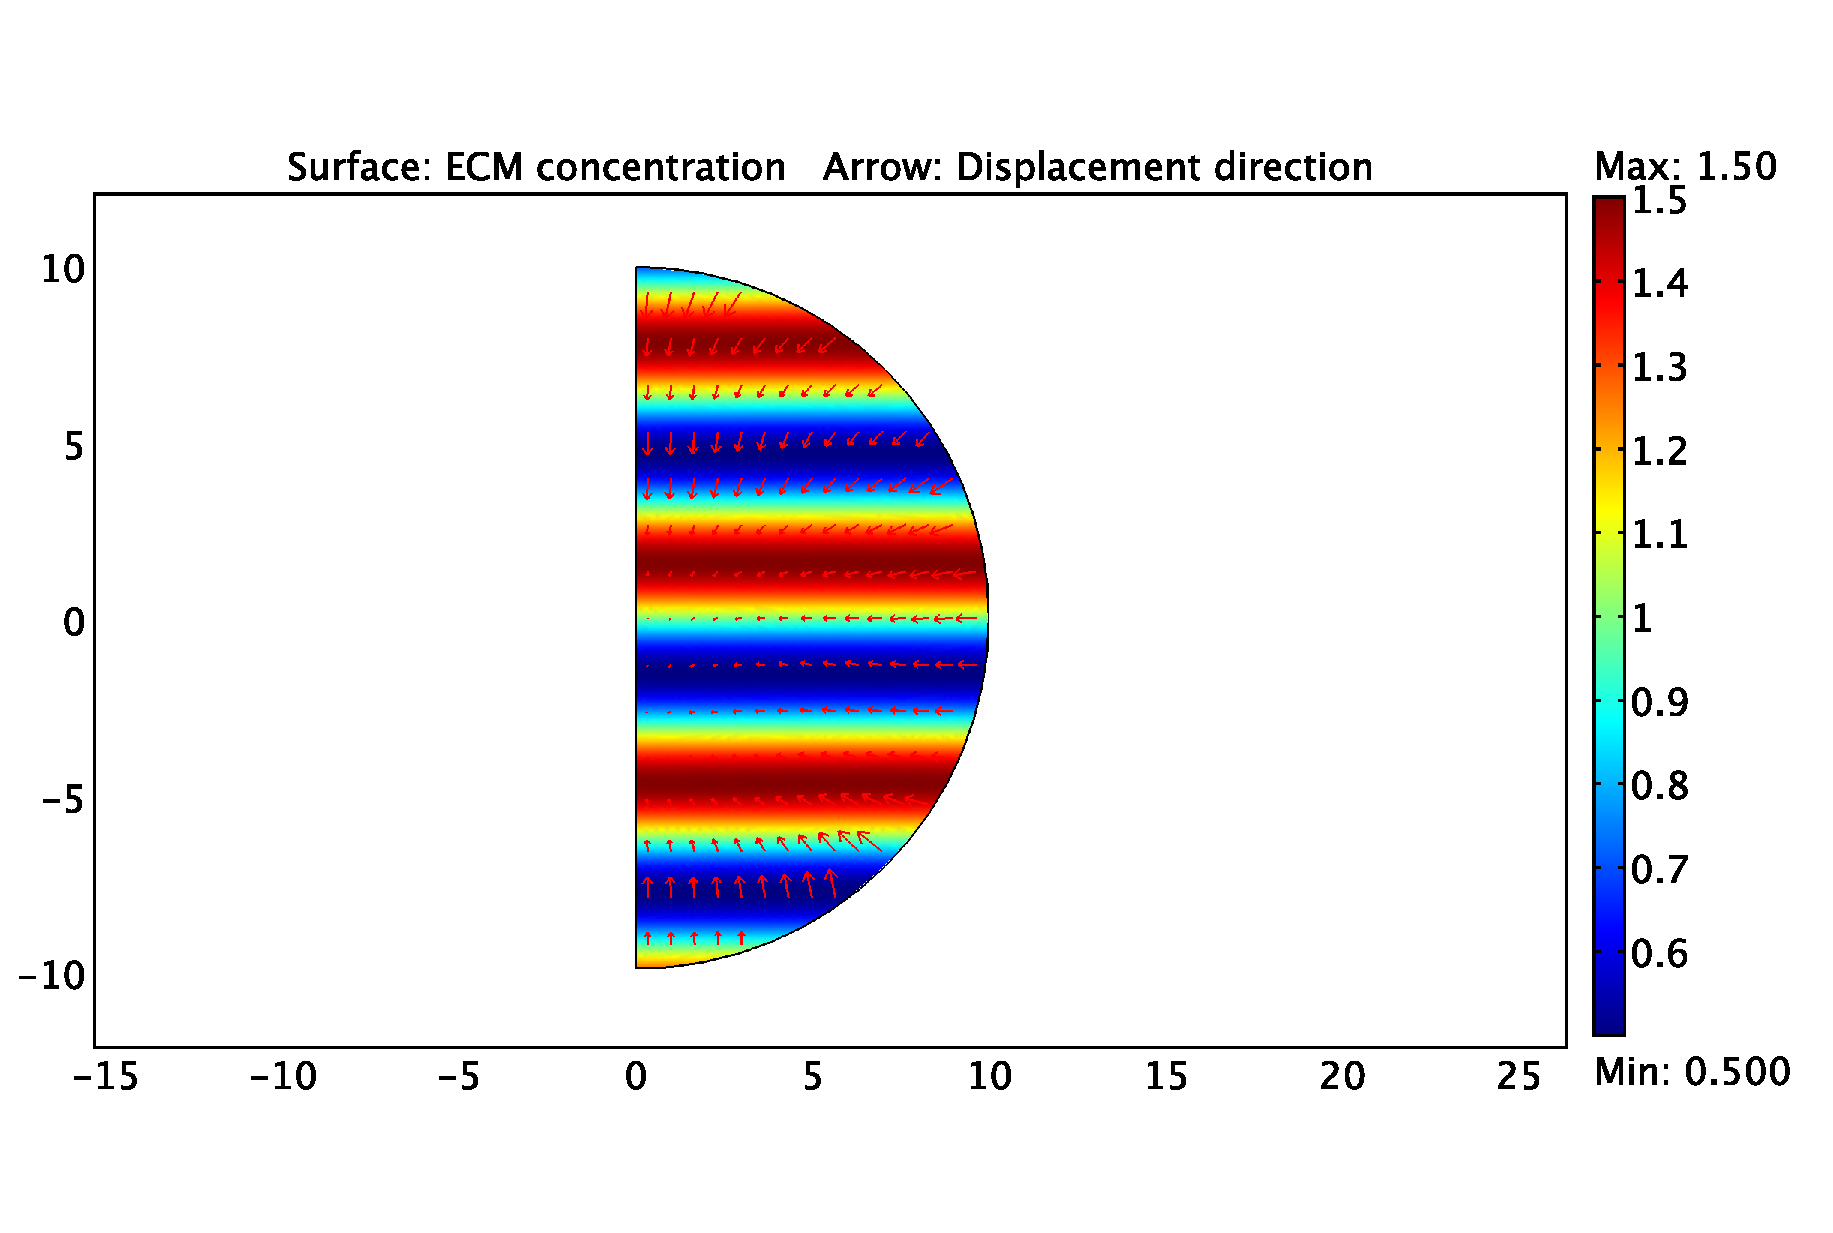
\includegraphics[width=0.8\textwidth]{images/examples/%
eulerian/cancer/heterogeneous-ecm-concentration}
\caption{Heterogeneous extra-cellular matrix concentration.}
\label{heterogeneous-ecm-concentration}
\end{figure}

\textbullet\ And with this, we have (apart from proliferating and
diffusing), heading toward areas of higher ECM. In these calculations,
growth (swelling) has been turned off and the arrows show the inward
tug. 

\begin{figure}[!hptb]
\centering
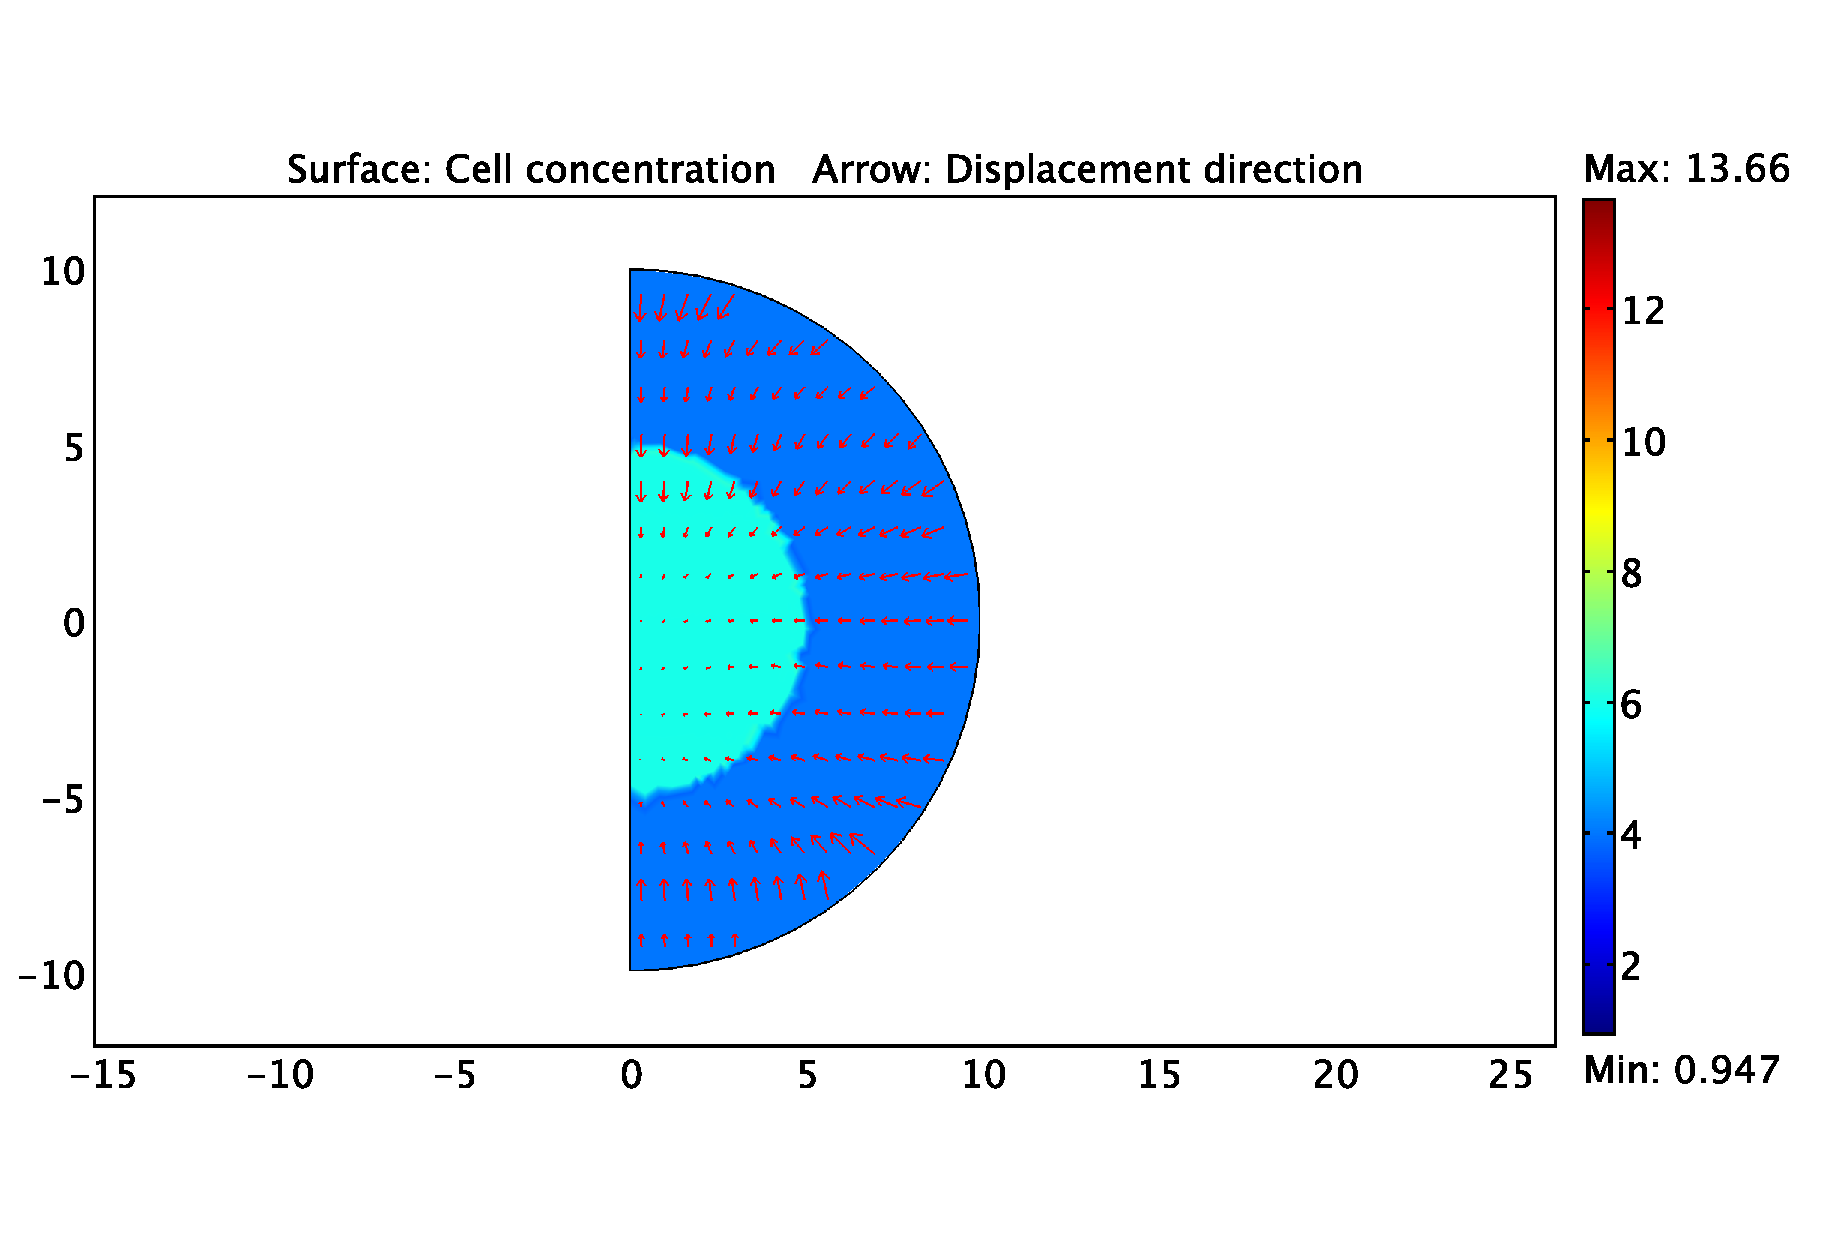
\includegraphics[width=0.8\textwidth]{images/examples/%
eulerian/cancer/haptotaxis-proliferating-cells-0}
\caption{Proliferating cells undergoing diffusion and haptotaxis at time $t=0$ days.}
\label{tumour-haptotaxis-proliferation-0}
\end{figure}

\begin{figure}[!hptb]
\centering
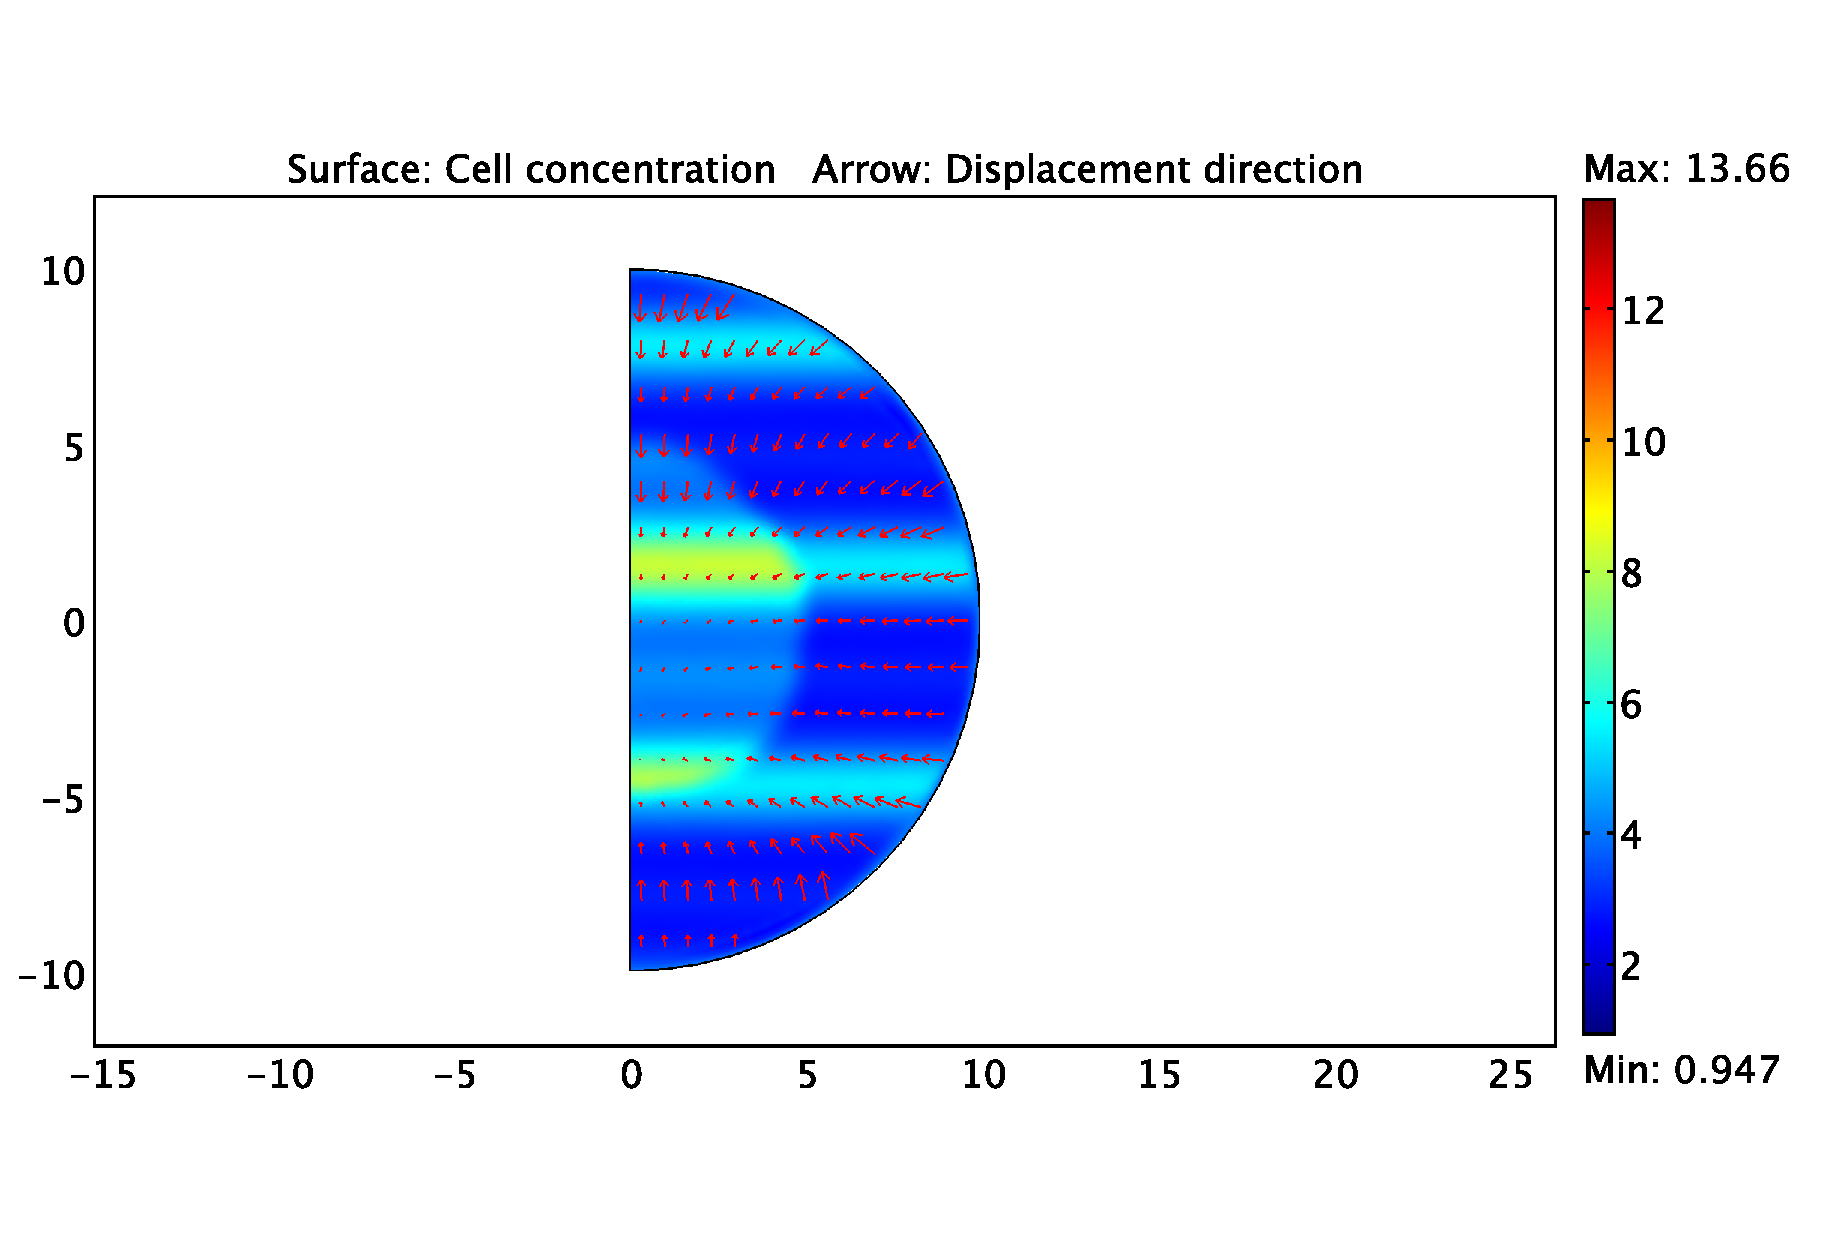
\includegraphics[width=0.8\textwidth]{images/examples/%
eulerian/cancer/haptotaxis-proliferating-cells-3p3}
\caption{Proliferating cells undergoing diffusion and haptotaxis at time $t=3.3$ days.}
\label{tumour-haptotaxis-proliferation-3p3}
\end{figure}

\begin{figure}[!hptb]
\centering
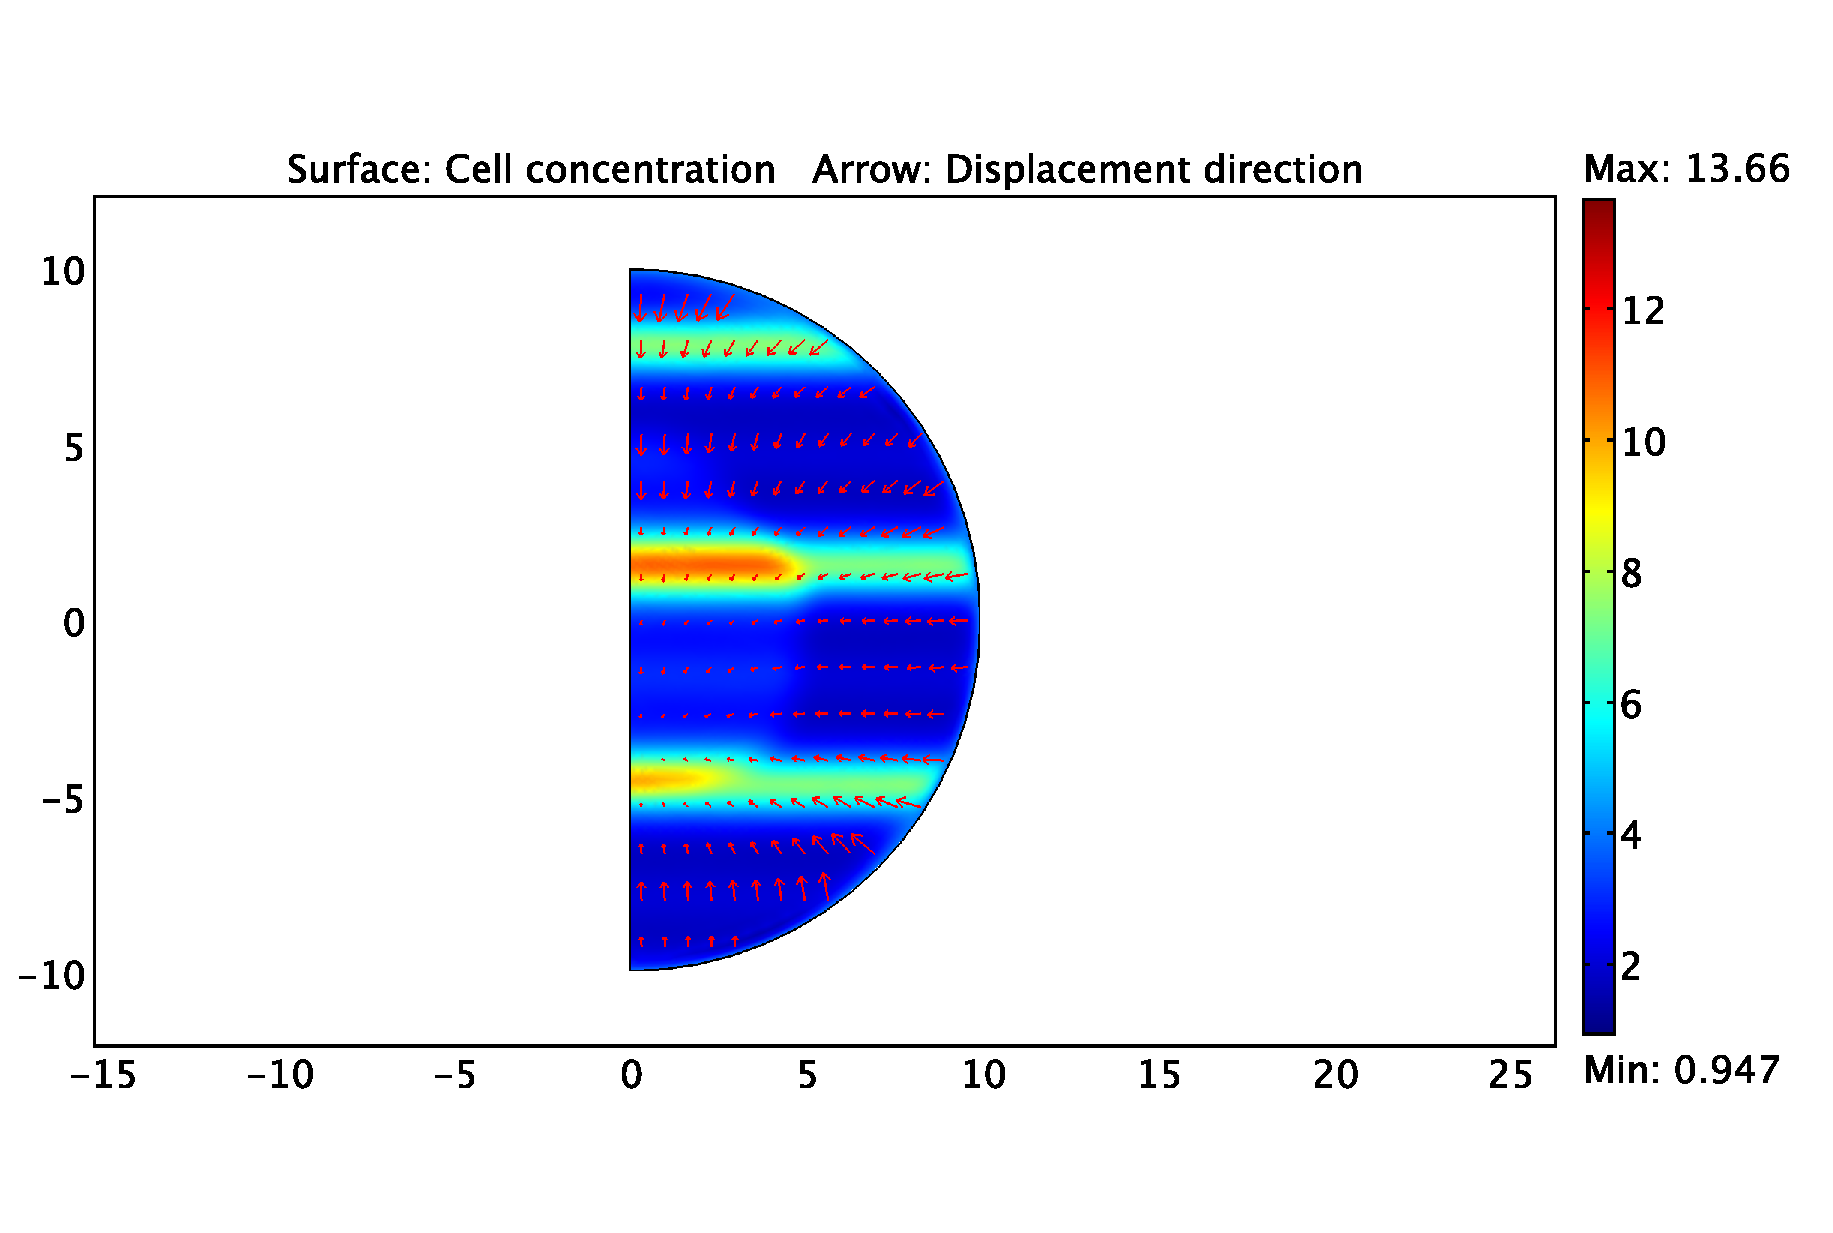
\includegraphics[width=0.8\textwidth]{images/examples/%
eulerian/cancer/haptotaxis-proliferating-cells-6p7}
\caption{Proliferating cells undergoing diffusion and haptotaxis at time $t=6.7$ days.}
\label{tumour-haptotaxis-proliferation-6p7}
\end{figure}

\begin{figure}[!hptb]
\centering
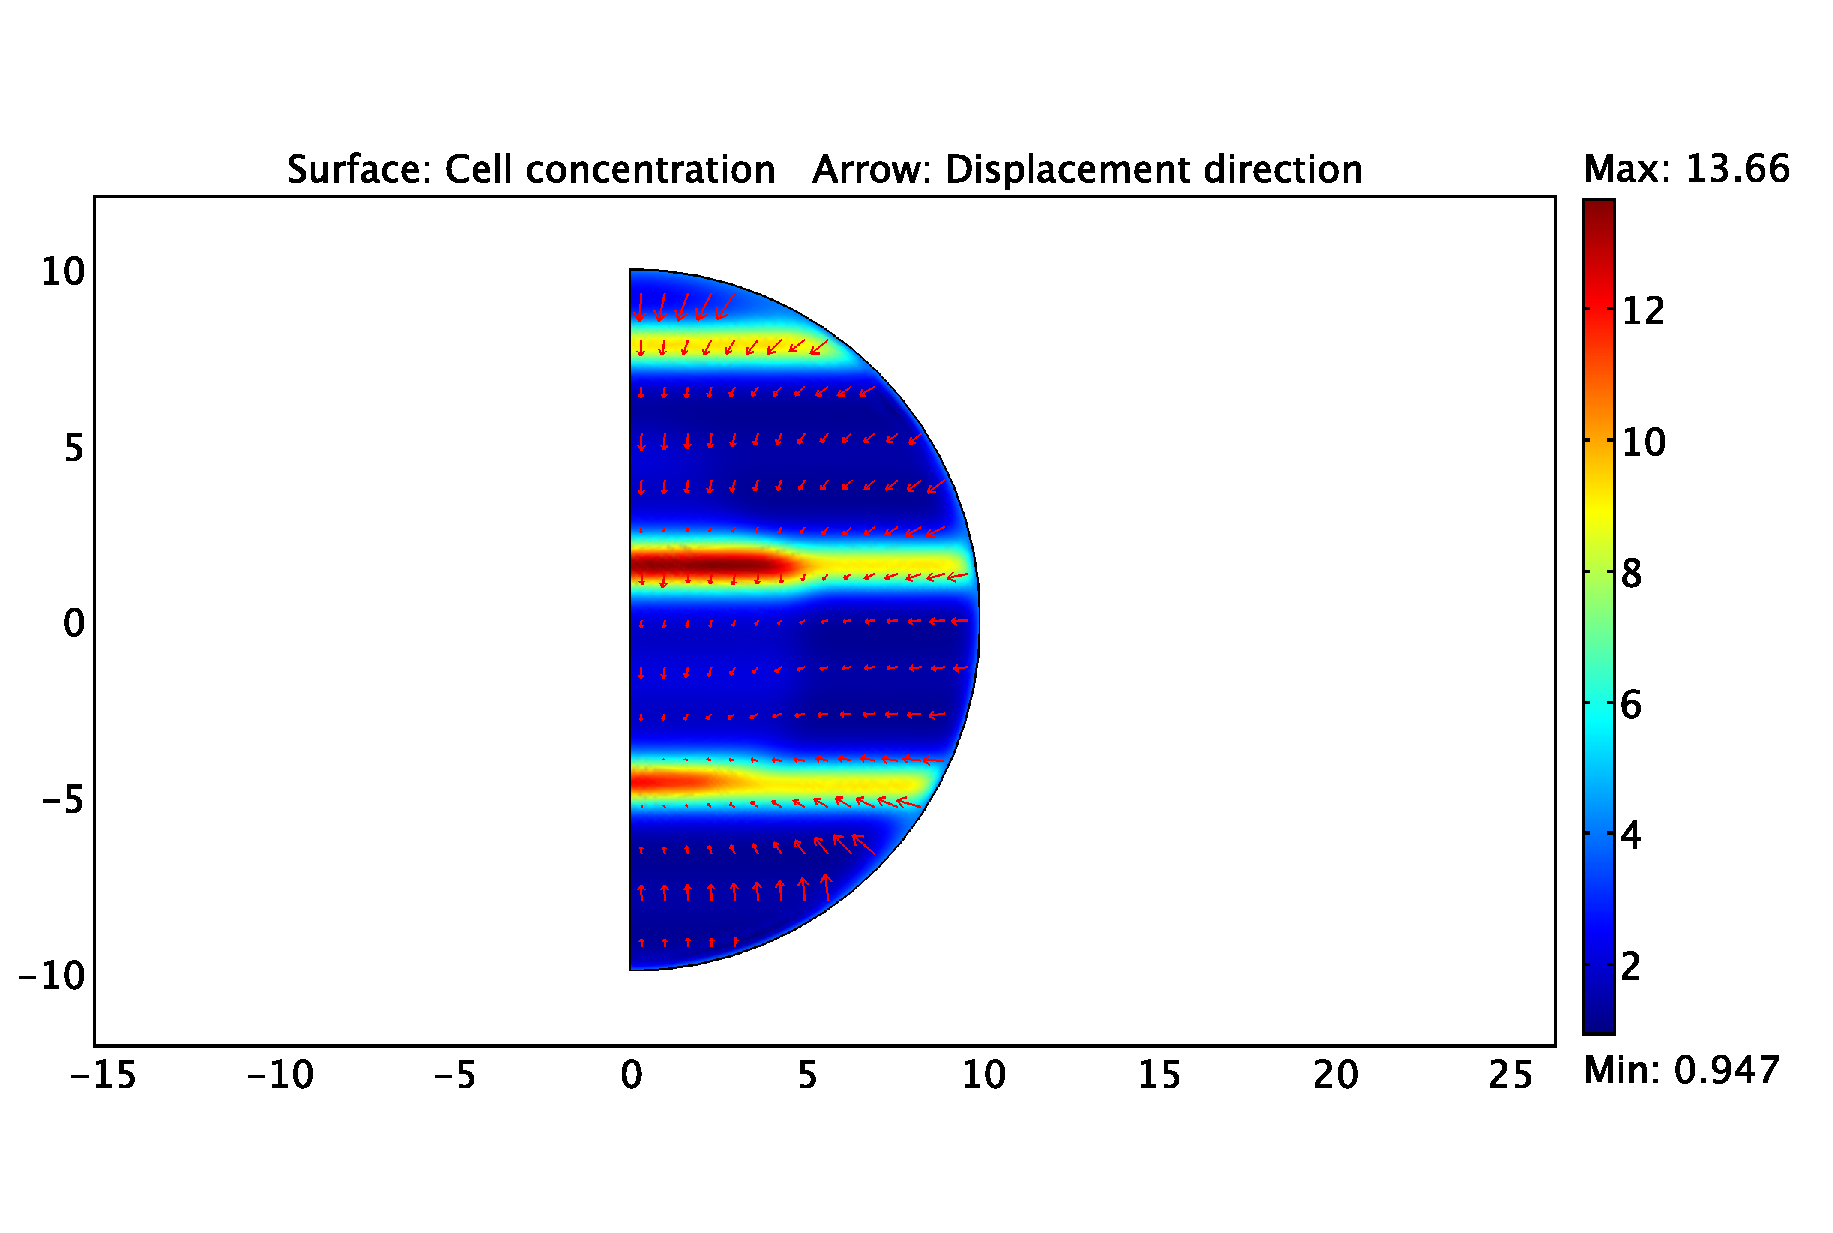
\includegraphics[width=0.8\textwidth]{images/examples/%
eulerian/cancer/haptotaxis-proliferating-cells-10}
\caption{Proliferating cells undergoing diffusion and haptotaxis at time $t=10$ days.}
\label{tumour-haptotaxis-proliferation-10}
\end{figure}

\clearpage

\subsection{Combining everything}
\label{cacophonous-medley}

\textbullet\ We are finally ready to solve the problem we described
initially. The range of physics incorporated here include, diffusing,
proliferating and haptotacting cells, growth induced by them and
swelling, nutrient is a constant field, growth follows a simple rate
law, soft contact mechanics introduced by the wall.

\textbullet\ Clearly, regions with more cells grow faster, and the
plots show the x-displacement as a measure of swelling. Also, the
presence of the wall biases the growth toward the top and bottom as
seen in experiment. Currently, all this arises out of a growth law
that's independent of stress (isotropic swelling), but with careful
experimental work its form can be fixed. Compare this to the case
where the growth happened without a wall.

\begin{figure}[!hptb]
\centering
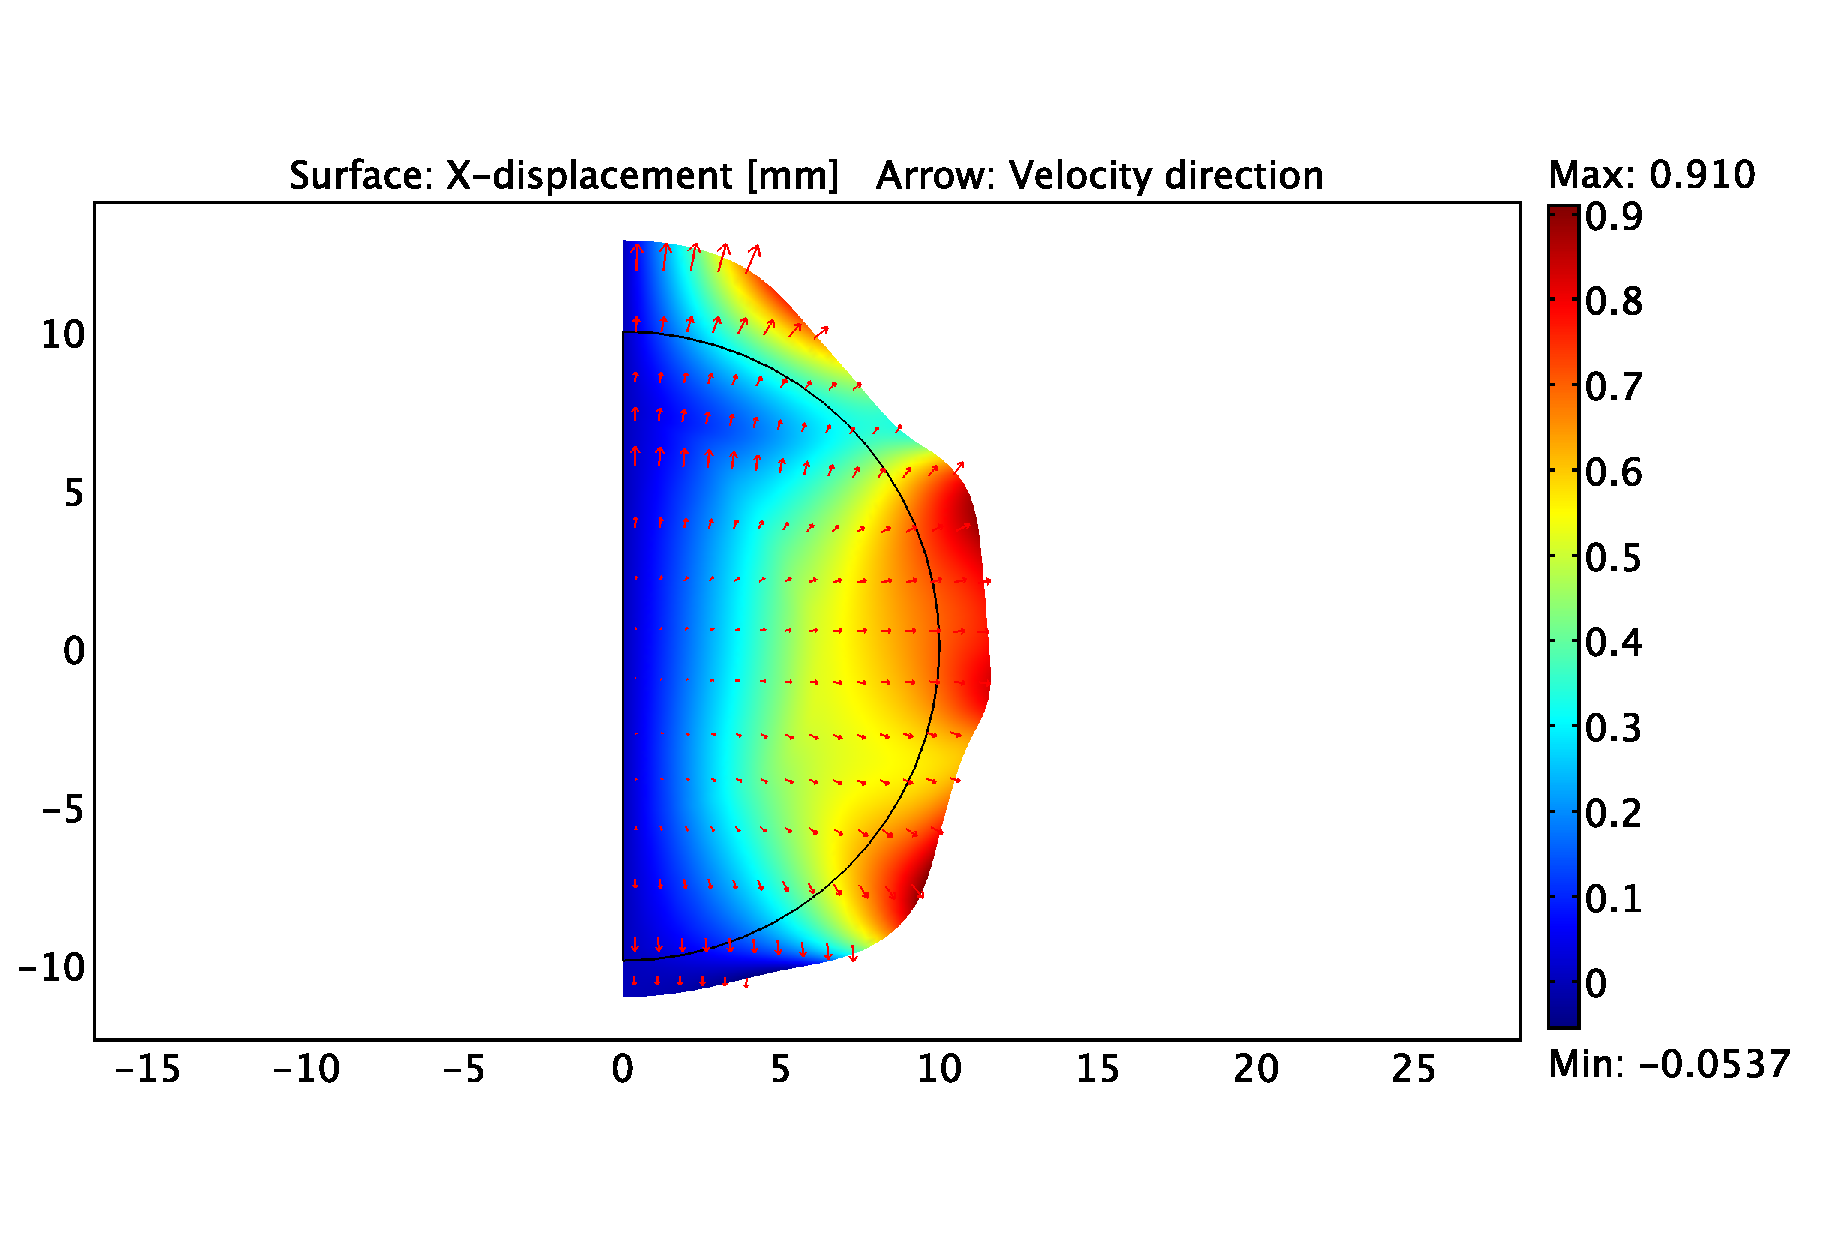
\includegraphics[width=0.8\textwidth]{images/examples/%
eulerian/cancer/growing-tumour-no-wall-4}
\caption{An unconstrained growing tumour at $t=4$ months.}
\label{tumour-growth-no-wall-4}
\end{figure}

\begin{figure}[!hptb]
\centering
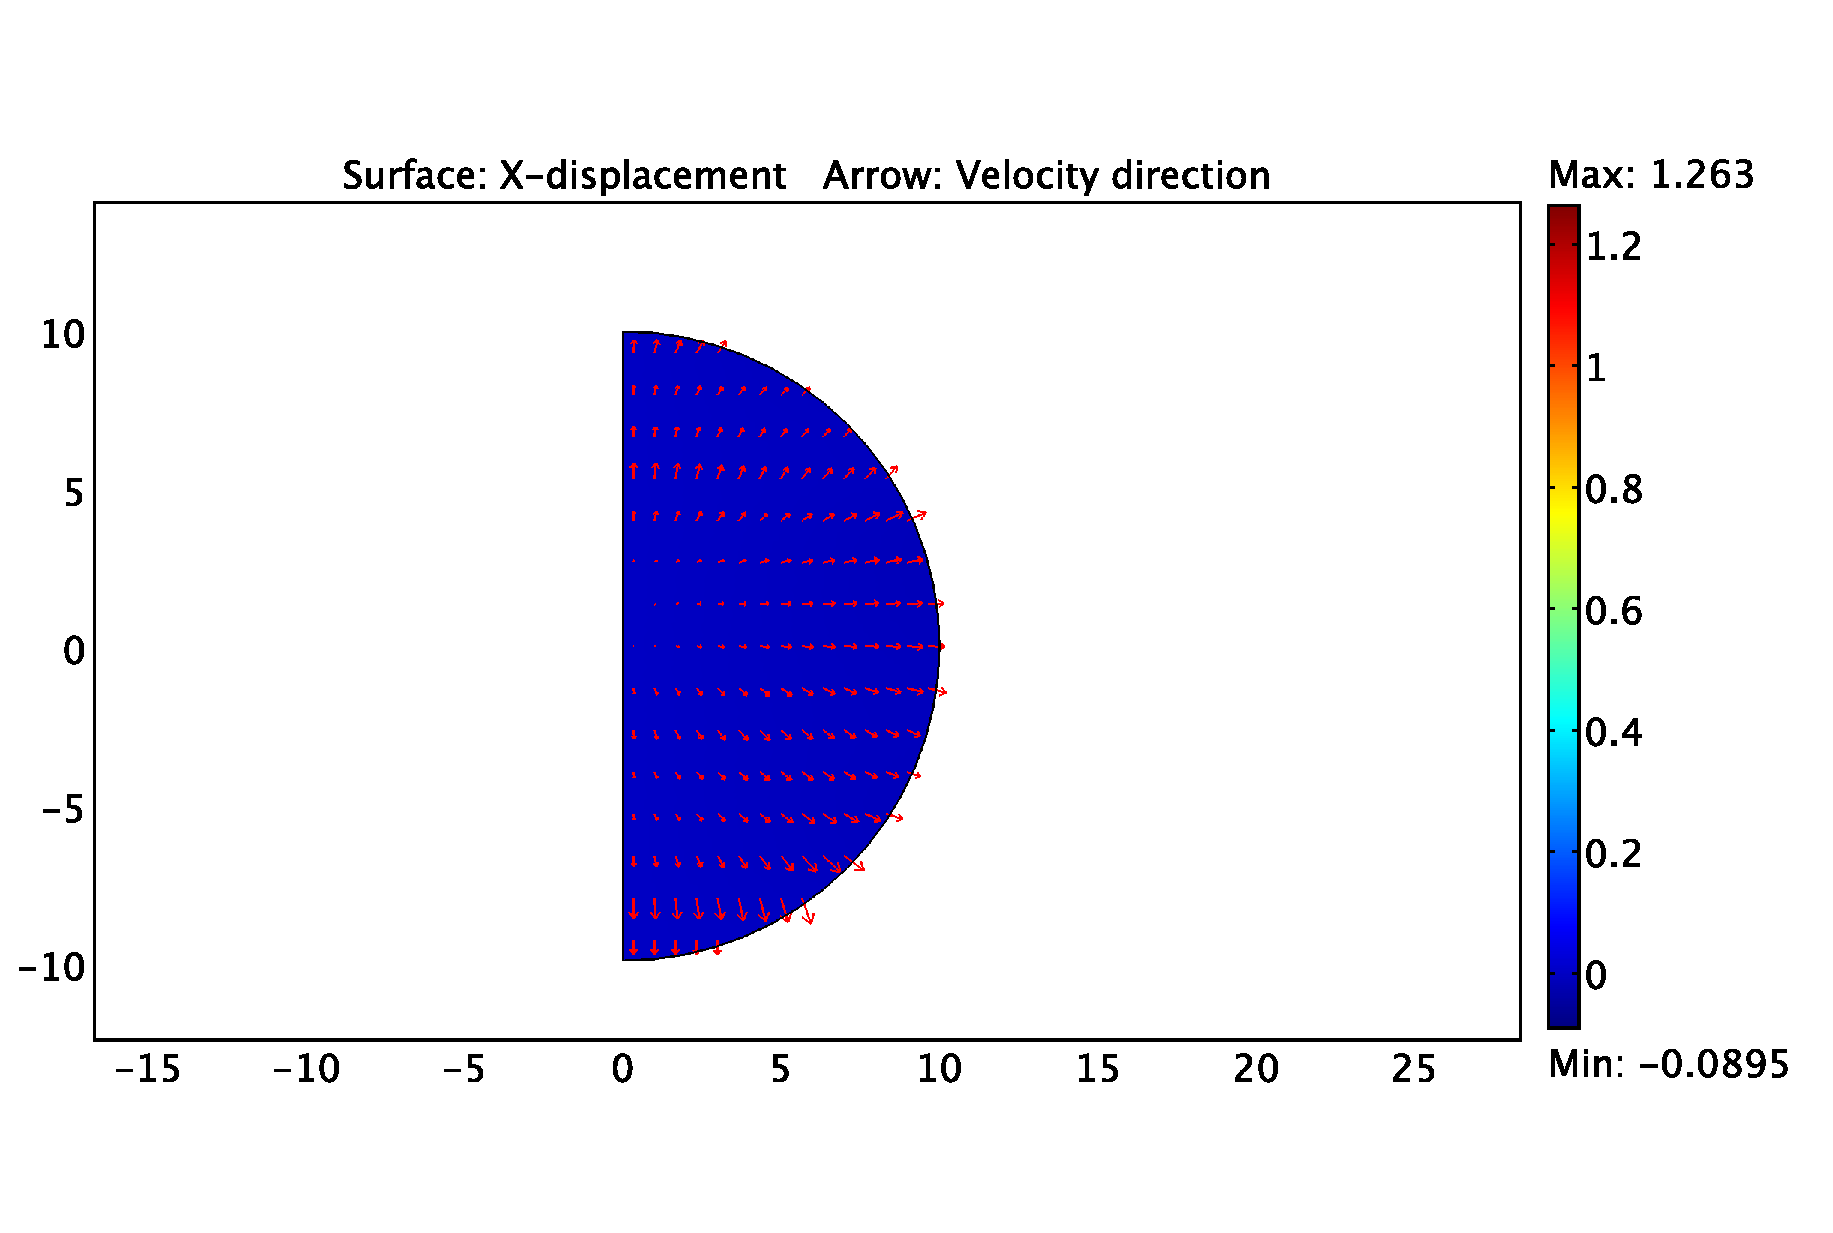
\includegraphics[width=0.8\textwidth]{images/examples/%
eulerian/cancer/growing-tumour-0.eps}
\caption{A constrained growing tumour at $t=0$ months.}
\label{tumour-growth-constrained-0}
\end{figure}

\begin{figure}[!hptb]
\centering
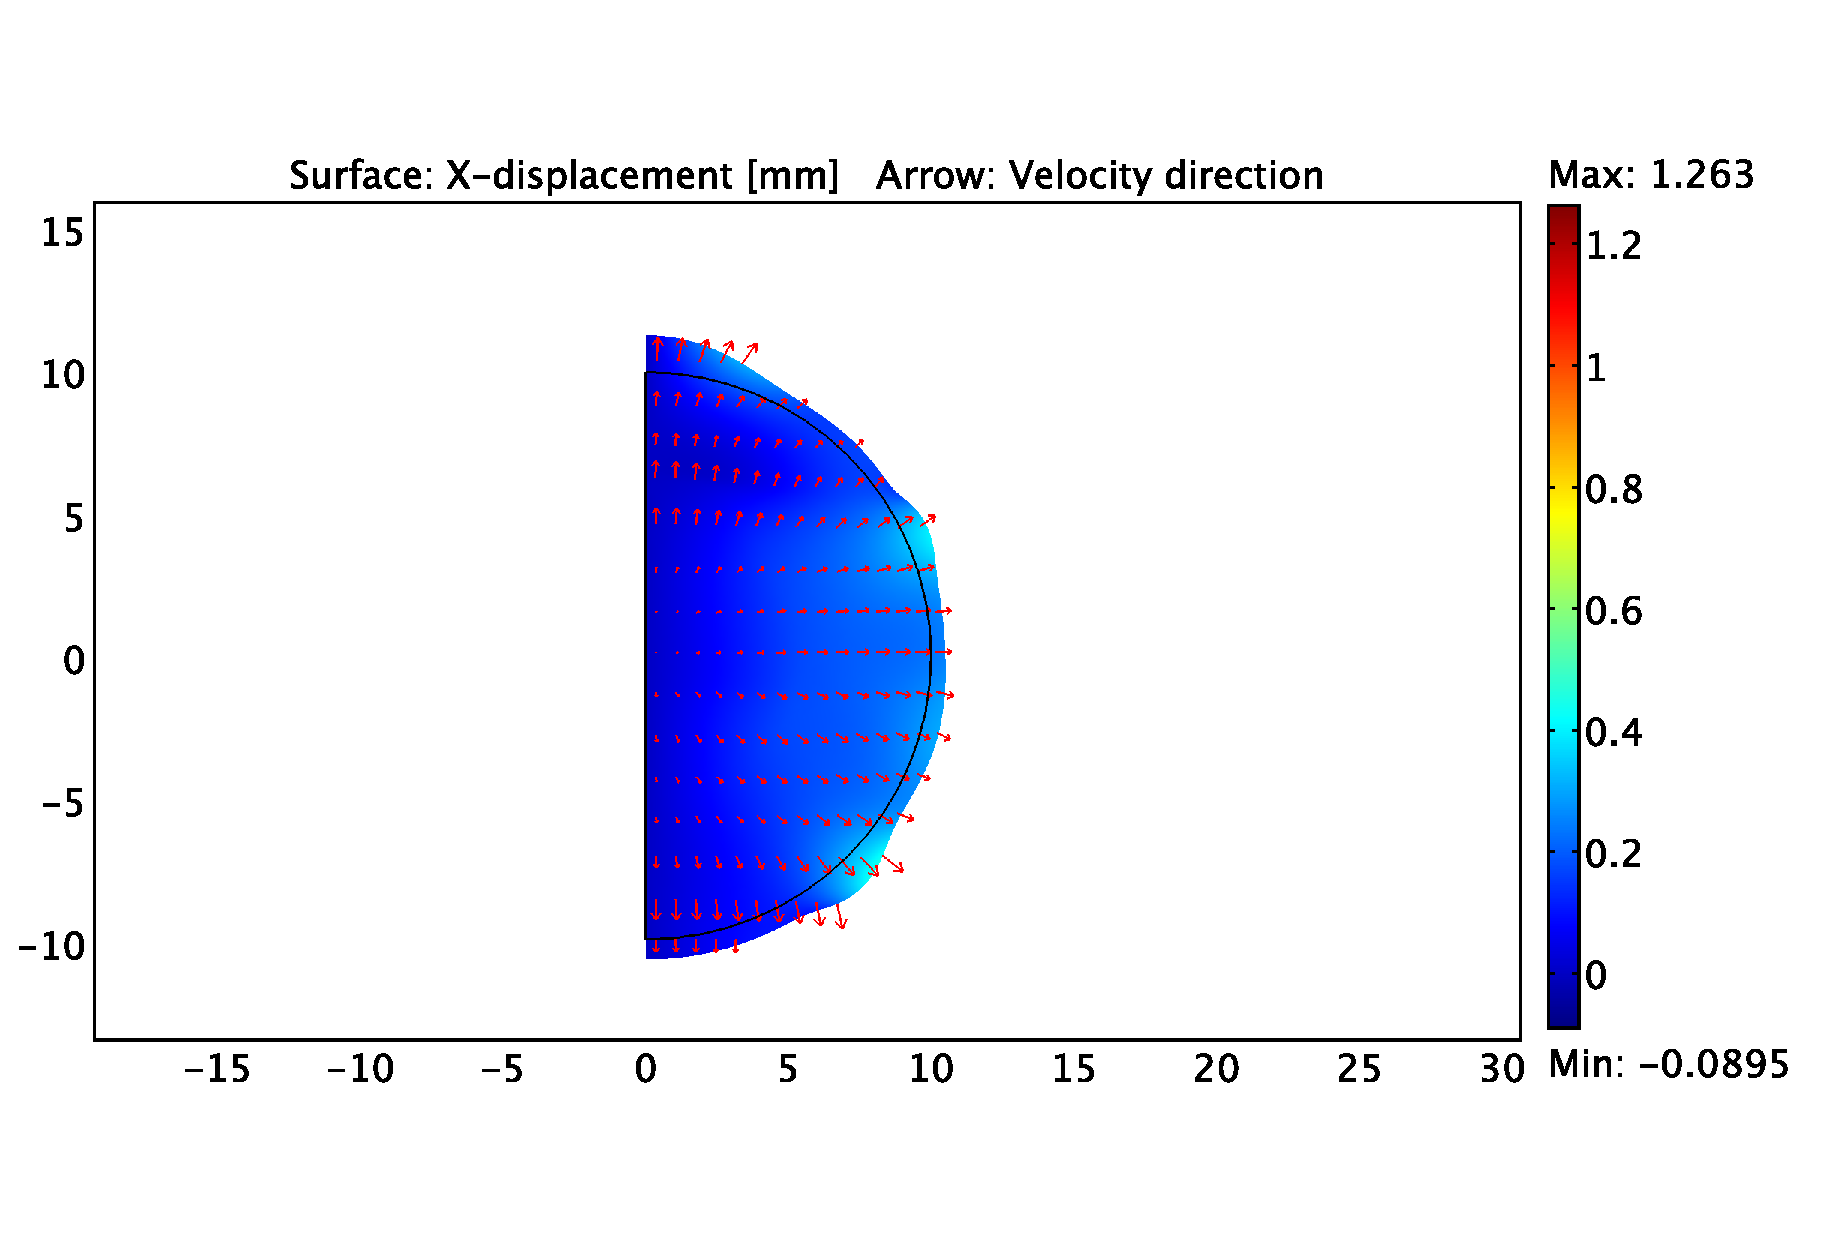
\includegraphics[width=0.8\textwidth]{images/examples/%
eulerian/cancer/growing-tumour-1.eps}
\caption{A constrained growing tumour at $t=1$ months.}
\label{tumour-growth-constrained-1}
\end{figure}

\begin{figure}[!hptb]
\centering
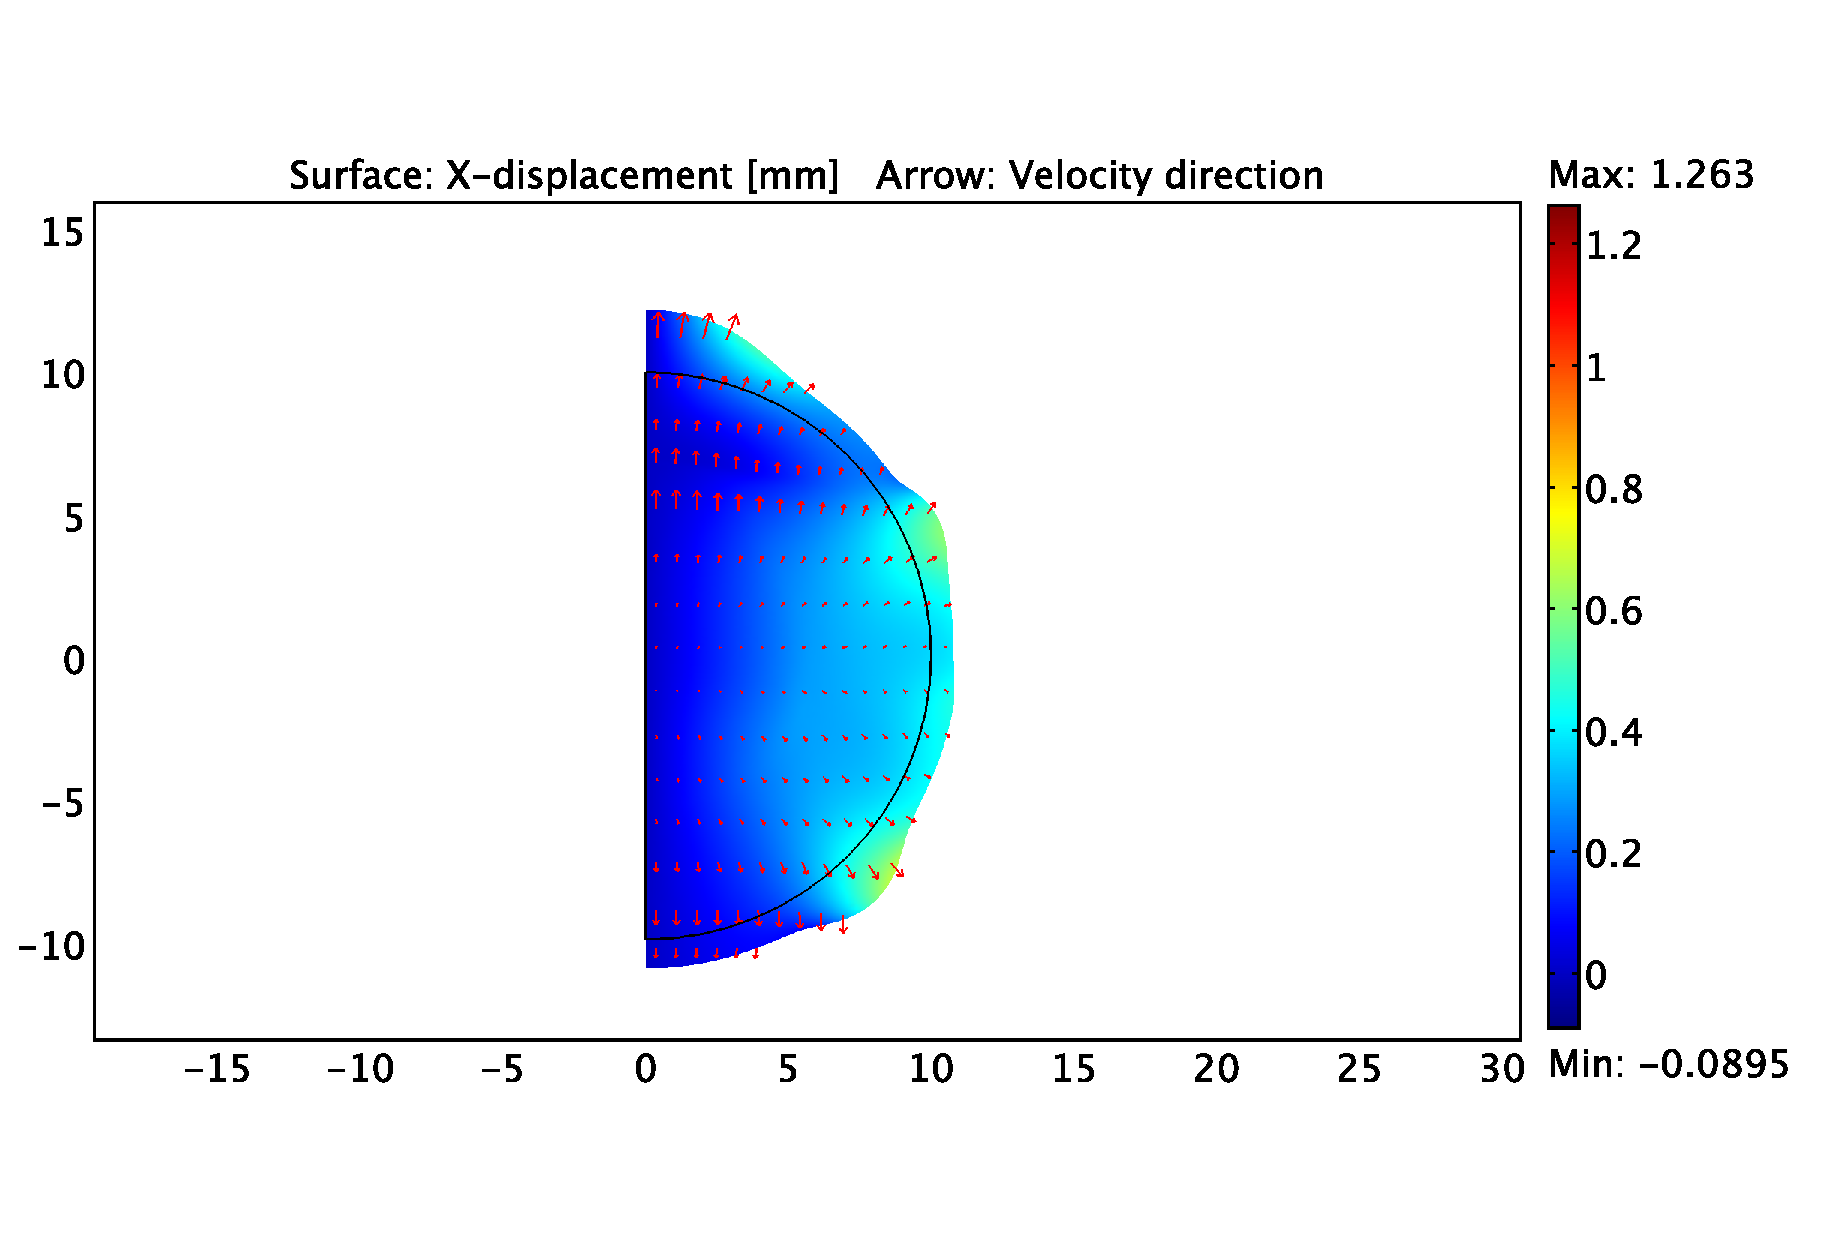
\includegraphics[width=0.8\textwidth]{images/examples/%
eulerian/cancer/growing-tumour-2.eps}
\caption{A constrained growing tumour at $t=2$ months.}
\label{tumour-growth-constrained-2}
\end{figure}

\begin{figure}[!hptb]
\centering
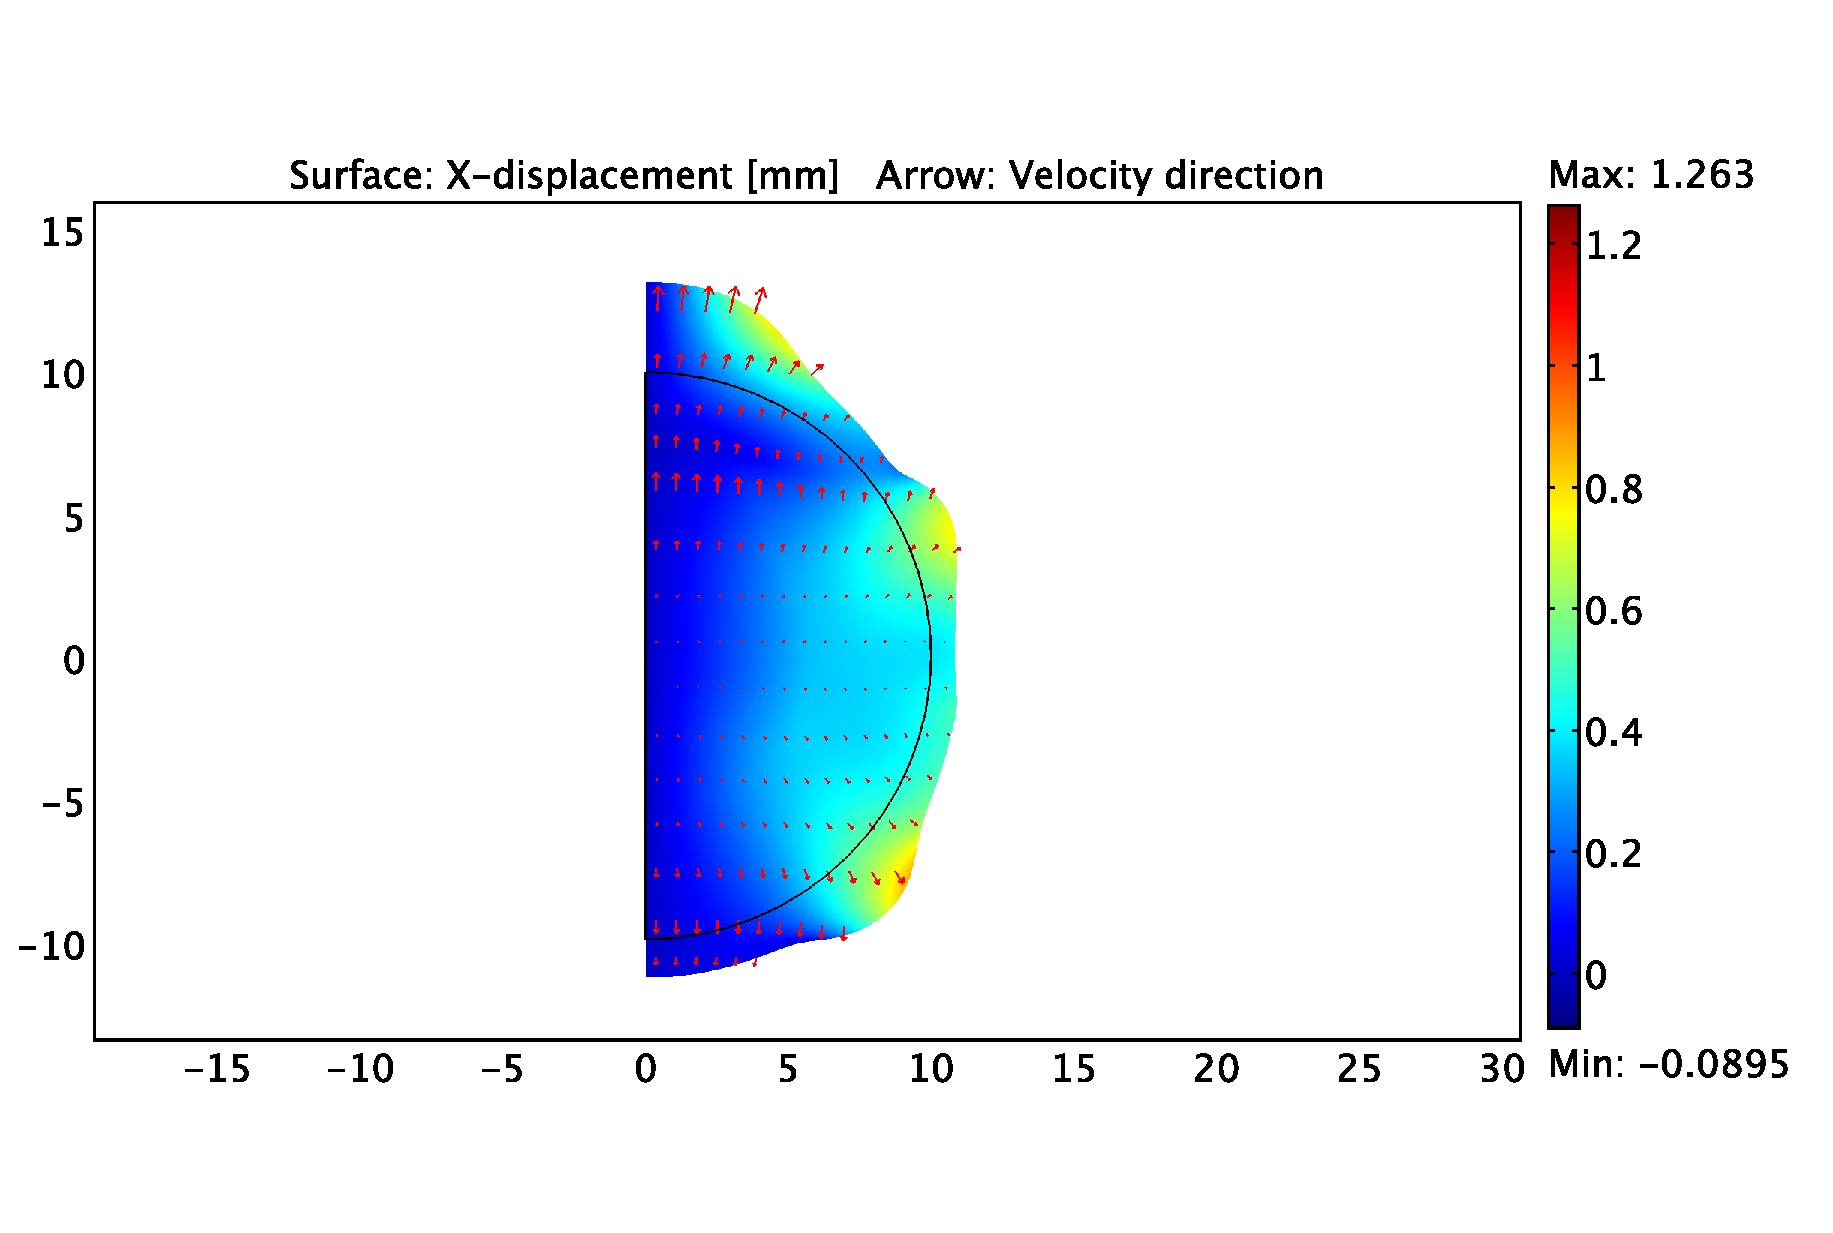
\includegraphics[width=0.8\textwidth]{images/examples/%
eulerian/cancer/growing-tumour-3.eps}
\caption{A constrained growing tumour at $t=3$ months.}
\label{tumour-growth-constrained-3}
\end{figure}

\begin{figure}[!hptb]
\centering
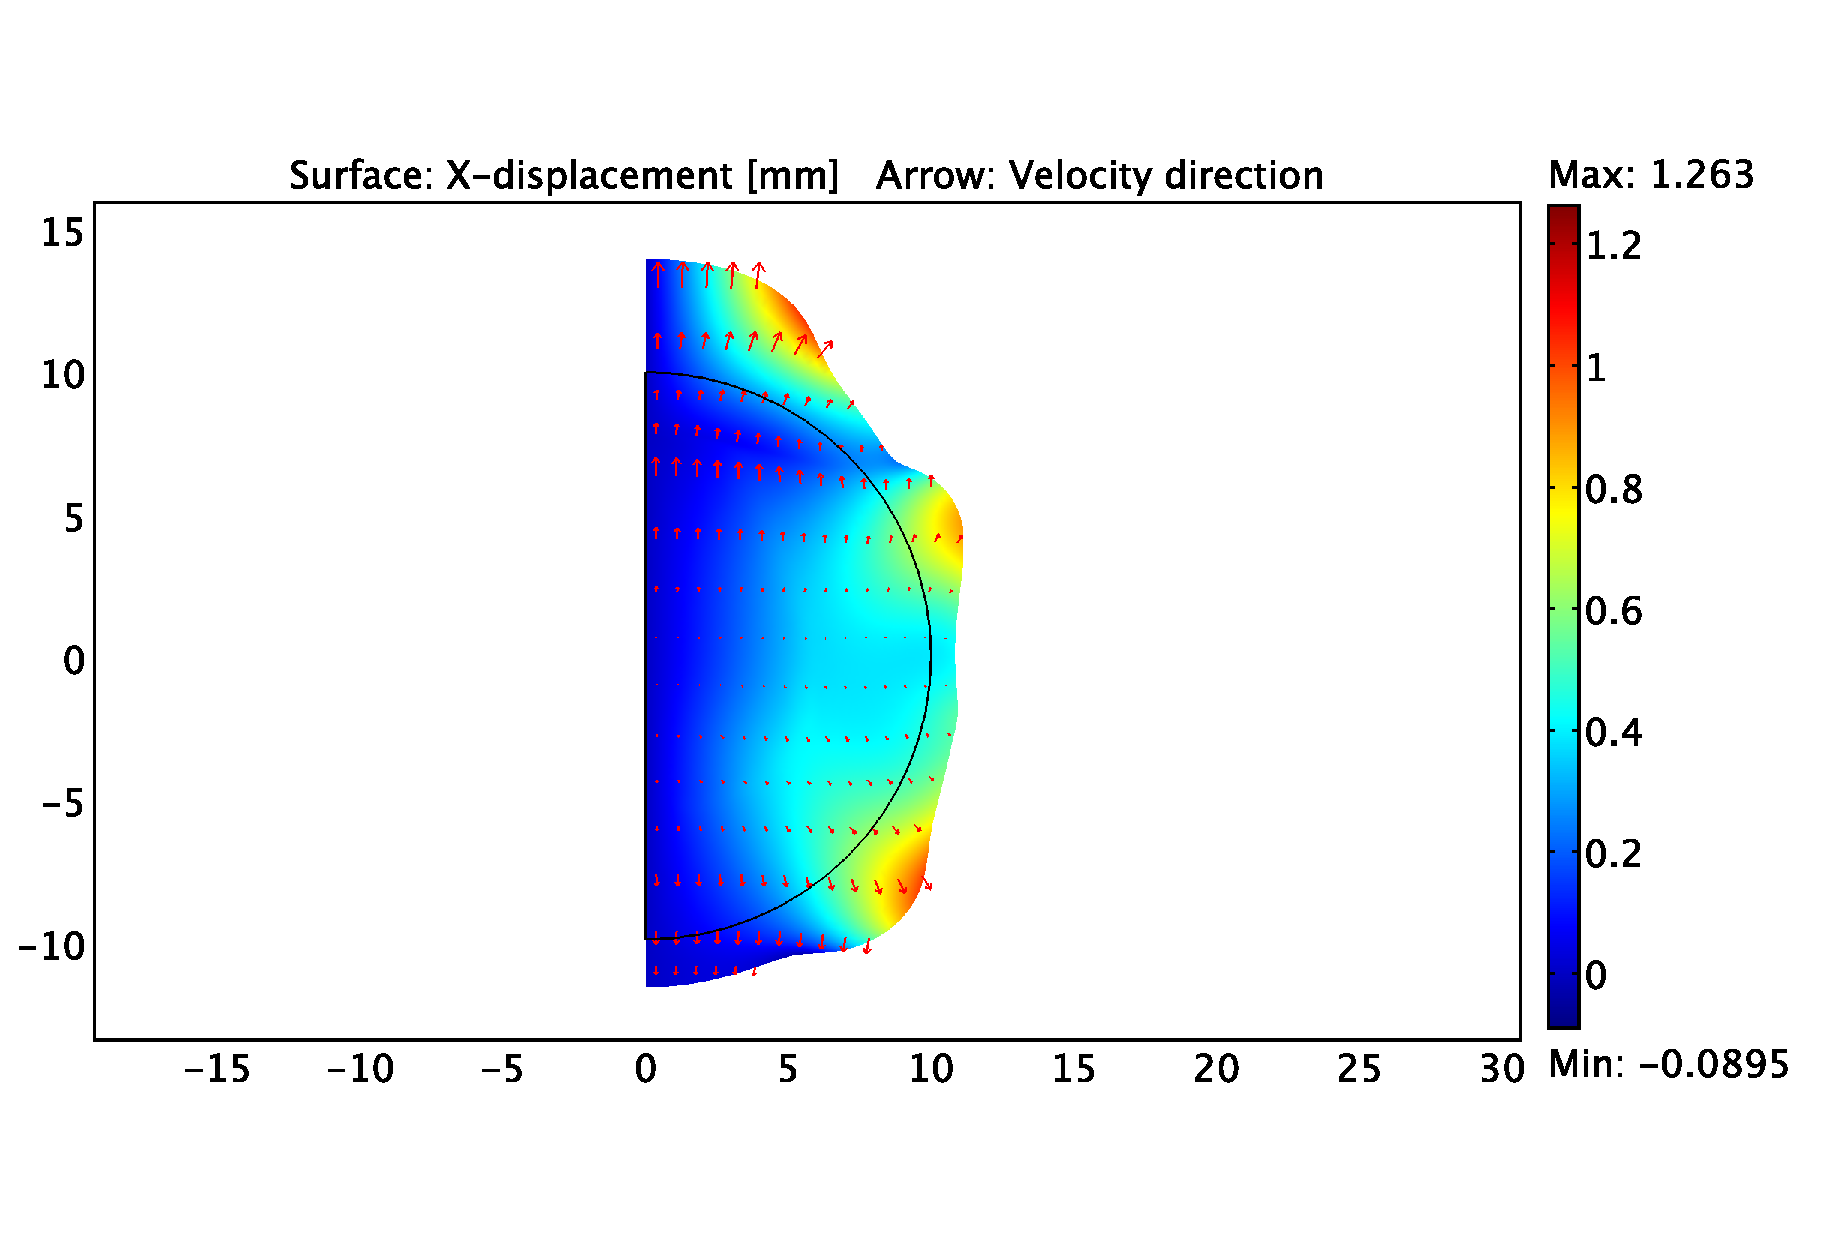
\includegraphics[width=0.8\textwidth]{images/examples/%
eulerian/cancer/growing-tumour-4.eps}
\caption{A constrained growing tumour at $t=4$ months.}
\label{tumour-growth-constrained-4}
\end{figure}

\begin{figure}[!hptb]
\centering
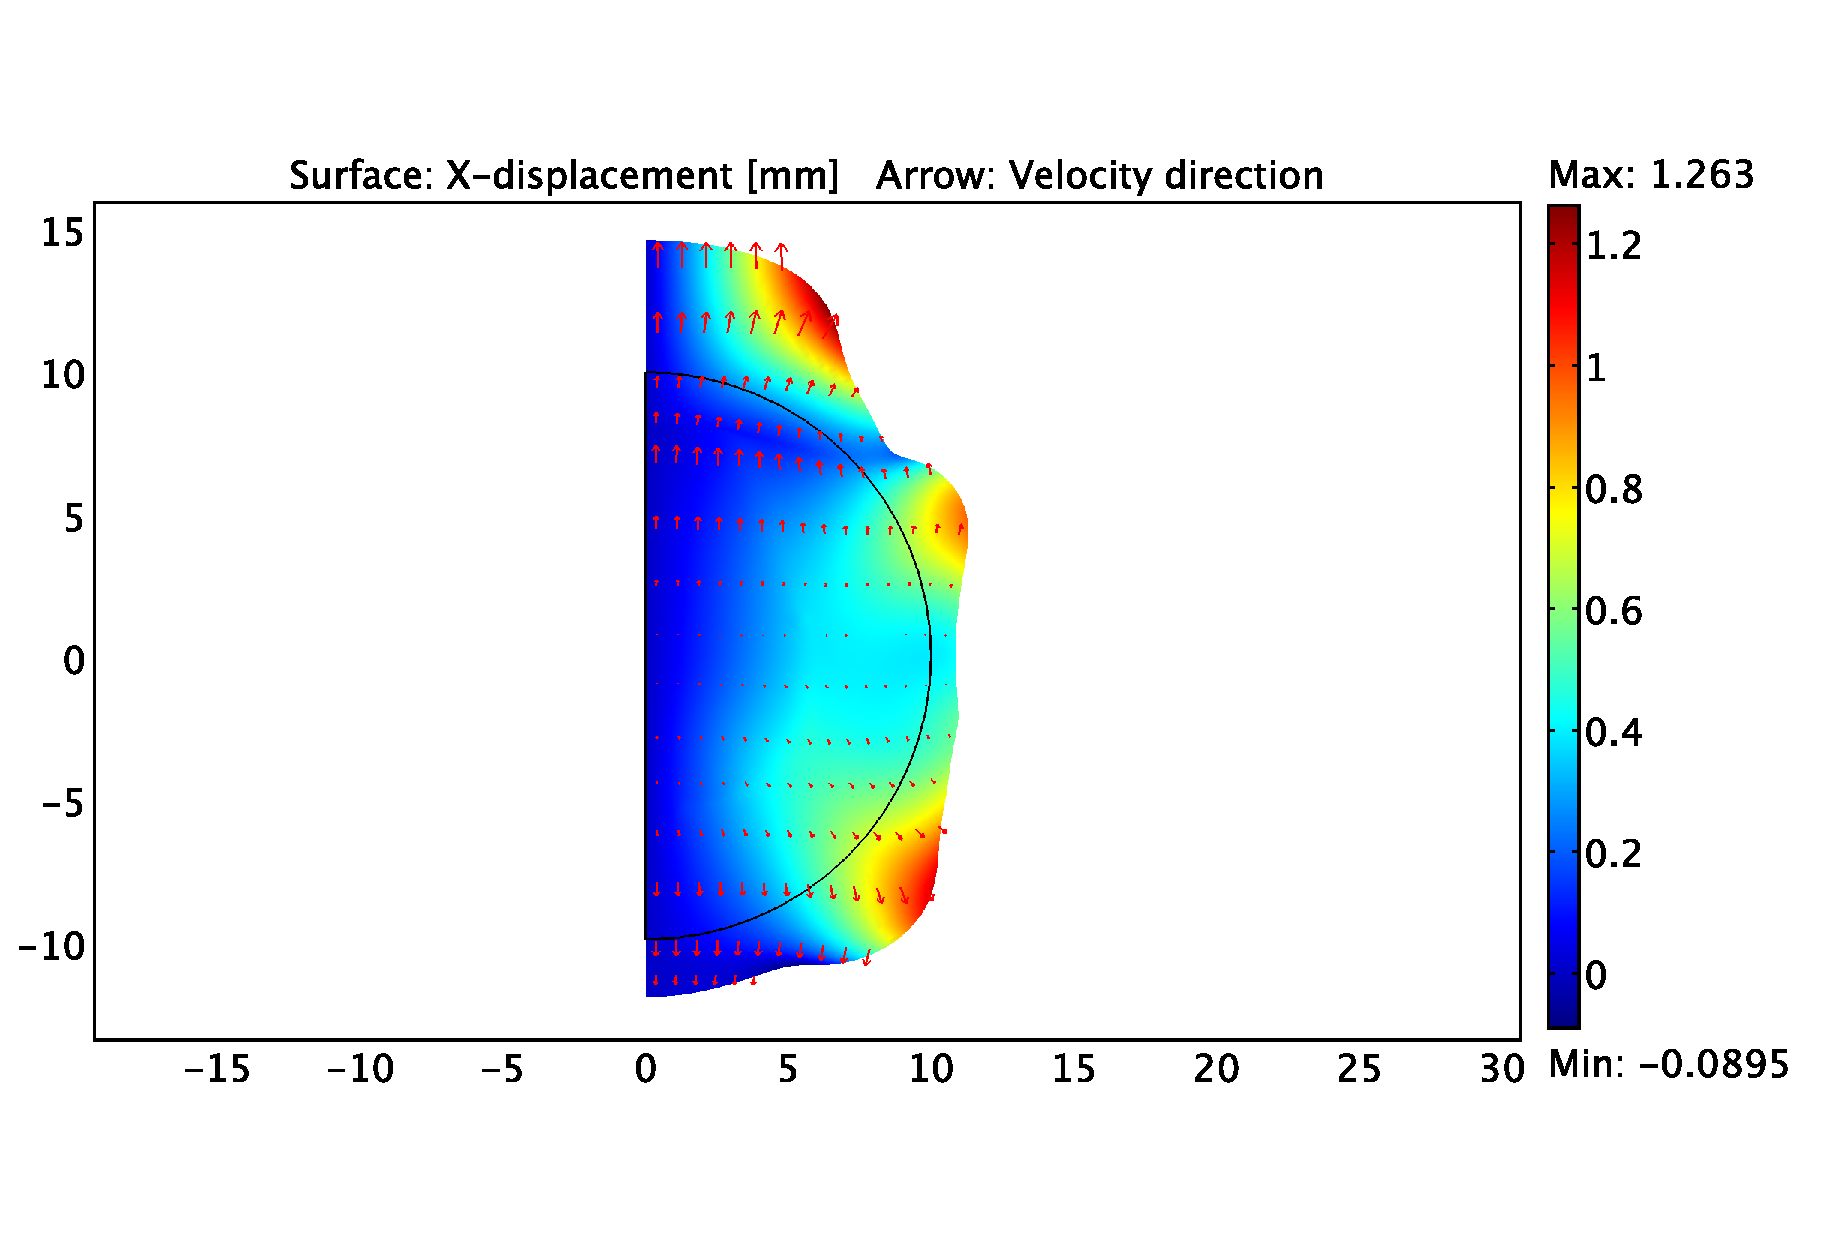
\includegraphics[width=0.8\textwidth]{images/examples/%
eulerian/cancer/growing-tumour-5.eps}
\caption{A constrained growing tumour at $t=5$ months.}
\label{tumour-growth-constrained-5}
\end{figure}

%% \todo{\begin{itemize}
%%     \item Talk about physically-relevant primitive variables and
%%       contrast choices with Chapter 3
%%   \item Weave around the monolithic implementation details and refer
%%     COMSOL's documentation. Cite back to the fact that monolithic
%%     is stable. Justify 2D.
%%   \item Generate pristine plots for the tensile-flow field
%%     calculations 
%%   \item Cite works from cancer literature to motivate the example. Tie
%%     in cell haptotaxis with gradients of other species 
%%   \item Talk about swelling boundary conditions and saturation
%%     constraint.
%%   \item Bring in a few experimental figures and point out what we're
%%     looking for in terms of biphasic response.
%% \end{itemize}}

% The move to the following perspective was motivated by the fact that
% the earlier formulation, and corresponding numerical examples (cite
% sections on role of mass balance in current conf., the deformation
% gradient split for the fluid, and the numerical example involving
% assumptions on deformation gradient of the fluid) involved
% quantities that, while reasonable from a 
% mathematical pint of view, did not correspond to physical quantities
% of interest in terms of physiological bvps. Point out that it's been
% 2--3 years of refining our understanding and trials with the
% previous code that's led to this point?


%

% Local Variables:
% TeX-master: "thesis"
% mode: latex
% mode: flyspell
% End:
